
% $Header: /Users/simon/common/docencia/ism/2011/RCS/ism.tex,v 1.1 2011/03/24 02:47:22 simon Exp simon $


\documentclass[handout,compress,english,10pt]{beamer}
%\documentclass[handout, compress,english,10pt]{extarticle}
%\usepackage{beamerarticle}


\newlength{\figheight}
\setlength{\figheight}{\textheight}  % for adjusting in articler mode (SIMON DEV)

\newlength{\figheightscl}
\setlength{\figheightscl}{0.7\textheight}  % for adjusting in articler mode (SIMON DEV)

\newlength{\figwidth}
\setlength{\figwidth}{\textwidth}  % for adjusting in articler mode (SIMON DEV)

%\def\figwidth{\textwidth}  % for adjusting in articler mode (SIMON DEV)
%\def\figheight{\textheight}
%\def\figheightscl{0.7\textheight}  % for adjusting in articler mode (SIMON DEV)
%
\usepackage{pgfpages}
\pgfpagesuselayout{2 on 1}[letterpaper, border, shrink=5mm]

% This file merged from solution template for talk is between 15min
% and 45min long,
% /sw/etc/texmf.local/doc/latex/beamer/solutions/generic-talks:
% and /sw/etc/texmf.local/doc/latex/beamer/examples/a-lecture/

% Copyright 2007 by Till Tantau
%
% This file may be distributed and/or modified
%
% 1. under the LaTeX Project Public License and/or
% 2. under the GNU Public License.
%
% See the file doc/licenses/LICENSE for more details.


% Common packages

\usepackage[english]{babel}
\usepackage[latin1]{inputenc}
\usepackage{times}
\mode<article>
{
  \usepackage{times}
  \usepackage{mathptmx}
  \usepackage[left=1.5cm,right=6cm,top=1.5cm,bottom=3cm]{geometry}
}

\usepackage{hyperref}
\usepackage[T1]{fontenc}
\usepackage{tikz}
\usepackage{colortbl}
\usepackage{yfonts}
\usepackage{colortbl}
%\usepackage{translator} % comment this, if not available


% Common settings for all lectures in this course

\def\lecturename{ISM}

\def\coursename{ISM}

\title{\insertlecture}

\author{Simon Casassus 
  Astronom\'{\i}a,  Universidad de Chile\\
 {\tt http:://www.das.uchile.cl/$\sim$simon}}

\institute
{       
\begin{columns}[t,onlytextwidth]

\column{0.5\textwidth}

\begin{description}[III]
\item[I]  Introduction:  Observations of the ISM
\item[II]  Microscopic Processes. % (ref. Dyson \& Williams + Spitzer + Shu).
\item[III]  Astrophysics of Gaseous Nebulae. % (ref. Osterbrock + review de Williams).
\end{description}

\column{0.5\textwidth}

\begin{description}[A]
\item[IV] Interstellar Dust.
\item[V] Dynamics of the ISM. 
\item[VI] Selectec topics: protoplanetary disks, planetary nebulae, SNRs.

\end{description}
%
\end{columns}
}

\subject{ \lecturename}

% Delete this, if you do not want the table of contents to pop up at
% the beginning of each subsection:
\AtBeginSubsection[]
{
  \begin{frame}<beamer>{Outline}
    \tableofcontents[currentsection,currentsubsection]
  \end{frame}
}


%\AtBeginSection[]
%{
%  \begin{frame}<beamer>{Outline}
%    \tableofcontents[currentsection] % ,currentsubsection
%  \end{frame}
%}


% Beamer version theme settings

\useoutertheme[height=0pt,width=2cm,right]{sidebar}
\usecolortheme{rose,sidebartab}
\useinnertheme{circles}
\usefonttheme[only large]{structurebold}

\setbeamercolor{sidebar right}{bg=black!15}
\setbeamercolor{structure}{fg=blue}
\setbeamercolor{author}{parent=structure}

\setbeamerfont{title}{series=\normalfont,size=\LARGE}
\setbeamerfont{title in sidebar}{series=\bfseries}
\setbeamerfont{author in sidebar}{series=\bfseries}
\setbeamerfont*{item}{series=}
\setbeamerfont{frametitle}{size=}
\setbeamerfont{block title}{size=\small}
\setbeamerfont{subtitle}{size=\normalsize,series=\normalfont}

\setbeamertemplate{navigation symbols}{}
\setbeamertemplate{bibliography item}[book]
\setbeamertemplate{sidebar right}
{
  {\usebeamerfont{title in sidebar}%
    \vskip1.5em%
    \hskip3pt%
    \usebeamercolor[fg]{title in sidebar}%
    \insertshorttitle[width=2cm,center,respectlinebreaks]\par%
    \vskip1.25em%
  }%
  {%
    \hskip3pt%
    \usebeamercolor[fg]{author in sidebar}%
    \usebeamerfont{author in sidebar}%
%    \insertshortauthor[width=2cm-2pt,center,respectlinebreaks]\par%
    \vskip1.25em%
  }%
  \hbox to2cm{\hss\insertlogo\hss}
  \vskip1.25em%
  \insertverticalnavigation{2cm}%
  \vfill
  \hbox to 2cm{\hfill\usebeamerfont{subsection in
      sidebar}\strut\usebeamercolor[fg]{subsection in
      sidebar}\insertshortlecture.\insertframenumber\hskip5pt}%
  \vskip3pt%
}%

\setbeamertemplate{title page}
{
  \vbox{}
  \vskip1em
%  {\huge Part  \insertshortlecture\par}
  {\usebeamercolor[fg]{title}\usebeamerfont{title}\inserttitle\par}%
  \ifx\insertsubtitle\@empty%
  \else%
    \vskip0.25em%
    {\usebeamerfont{subtitle}\usebeamercolor[fg]{subtitle}\insertsubtitle\par}%
  \fi%     
  \vskip1em\par
%   \insertdate\par
 % \vskip0pt plus1filll
\insertauthor\par
  \insertinstitute\vskip1em
}


%\setbeamertemplate{title page}
%{
%  \vbox{}
%  \vskip1em
%  {\huge Part  \insertshortlecture\par}
%  {\usebeamercolor[fg]{title}\usebeamerfont{title}\inserttitle\par}%
%  \ifx\insertsubtitle\@empty%
%  \else%
%    \vskip0.25em%
%    {\usebeamerfont{subtitle}\usebeamercolor[fg]{subtitle}\insertsubtitle\par}%
%  \fi%     
%  \vskip1em\par
%   \emph{\lecturename}\  \insertdate\par
%  \vskip0pt plus1filll
%  \leftskip=0pt plus1fill\insertauthor\par
%  \insertinstitute\vskip1em
%}
%
\logo{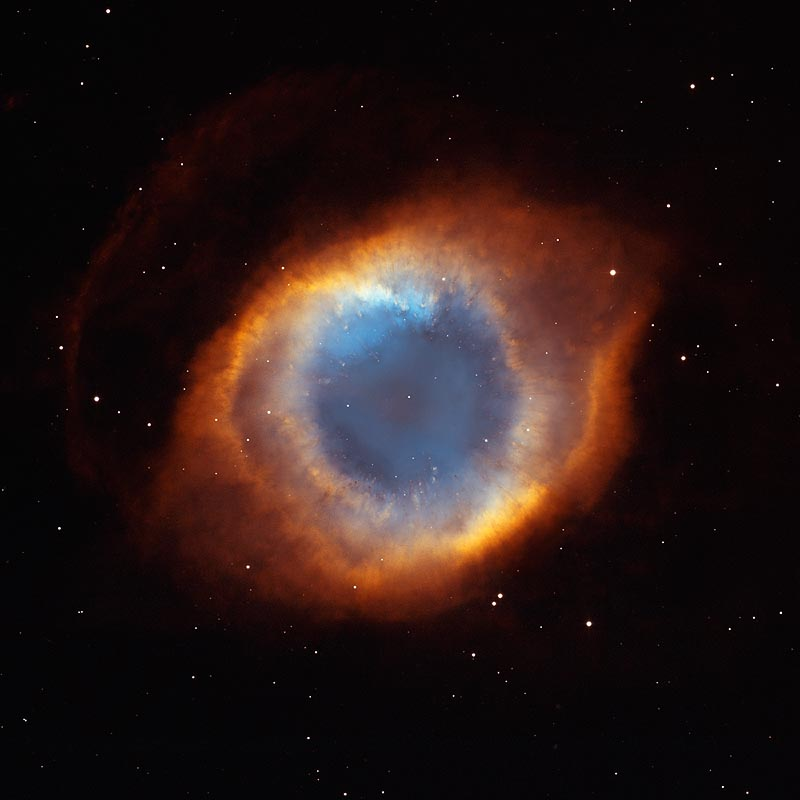
\includegraphics[width=2cm]{helix_hst.jpg}}



% Article version layout settings

\mode<article>

\makeatletter
\def\@listI{\leftmargin\leftmargini
  \parsep 0pt
  \topsep 5\p@   \@plus3\p@ \@minus5\p@
  \itemsep0pt}
\let\@listi=\@listI


\setbeamertemplate{frametitle}{\paragraph*{\insertframetitle\
    \ \small\insertframesubtitle}\ \par
}
\setbeamertemplate{frame end}{%
  \marginpar{\scriptsize\hbox to 1cm{\sffamily%
      \hfill\strut\insertshortlecture.\insertframenumber}\hrule height .2pt}}
\setlength{\marginparwidth}{1cm}
\setlength{\marginparsep}{4.5cm}

\def\@maketitle{\makechapter}

\def\makechapter{
  \newpage
  \null
  \vskip 2em%
  {%
    \parindent=0pt
    \raggedright
    \sffamily
    \vskip8pt
    {\fontsize{36pt}{36pt}\selectfont Kapitel \insertshortlecture \par\vskip2pt}
    {\fontsize{24pt}{28pt}\selectfont \color{blue!50!black} \insertlecture\par\vskip4pt}
    {\Large\selectfont \color{blue!50!black} \insertsubtitle\par}
    \vskip10pt

    \normalsize\selectfont Druckfassung der
    Vorlesung \emph{\lecturename} vom \@date\par\vskip1.5em
    \hfill Till Tantau, Institut f�r Theoretische Informatik, Universit�t zu L�beck
  }
  \par
  \vskip 1.5em%
}

\let\origstartsection=\@startsection
\def\@startsection#1#2#3#4#5#6{%
  \origstartsection{#1}{#2}{#3}{#4}{#5}{#6\normalfont\sffamily\color{blue!50!black}\selectfont}}

\makeatother

\mode
<all>




% Typesetting Listings

\usepackage{listings}
\lstset{language=Java}

\alt<presentation>
{\lstset{%
  basicstyle=\footnotesize\ttfamily,
  commentstyle=\slshape\color{green!50!black},
  keywordstyle=\bfseries\color{blue!50!black},
  identifierstyle=\color{blue},
  stringstyle=\color{orange},
  escapechar=\#,
  emphstyle=\color{red}}
}
{
  \lstset{%
    basicstyle=\ttfamily,
    keywordstyle=\bfseries,
    commentstyle=\itshape,
    escapechar=\#,
    emphstyle=\bfseries\color{red}
  }
}



% Common theorem-like environments

\theoremstyle{definition}
\newtheorem{exercise}[theorem]{\translate{Exercise}}




% New useful definitions:

\newbox\mytempbox
\newdimen\mytempdimen

\newcommand\includegraphicscopyright[3][]{%
  \leavevmode\vbox{\vskip3pt\raggedright\setbox\mytempbox=\hbox{\includegraphics[#1]{#2}}%
    \mytempdimen=\wd\mytempbox\box\mytempbox\par\vskip1pt%
    \fontsize{3}{3.5}\selectfont{\color{black!25}{\vbox{\hsize=\mytempdimen#3}}}\vskip3pt%
}}

\newenvironment{colortabular}[1]{\medskip\rowcolors[]{1}{blue!20}{blue!10}\tabular{#1}\rowcolor{blue!40}}{\endtabular\medskip}

\def\equad{\leavevmode\hbox{}\quad}

\newenvironment{greencolortabular}[1]
{\medskip\rowcolors[]{1}{green!50!black!20}{green!50!black!10}%
  \tabular{#1}\rowcolor{green!50!black!40}}%
{\endtabular\medskip}







\usepackage{wrapfig}


\usepackage{amsmath}
\usepackage{amssymb}
\usepackage{amsfonts}
\usepackage{latexsym}


\usepackage{floatflt}                          

\def\ls{\stackrel{<}{\small \sim}}
\def\gs{\stackrel{>}{\small \sim}}

%\def\gs{\mathrel{\raise1.16pt\hbox{$>$}\kern-7.0pt
%\lower3.06pt\hbox{{$\scriptstyle \sim$}}}}
%\def\ls{\mathrel{\raise1.16pt\hbox{$<$}\kern-7.0pt
%\lower3.06pt\hbox{{$\scriptstyle \sim$}}}}

%usepackage{pause}                          %required for ppower4
%usepackage[bgadd]{background}                     %required for ppower4
%usepackage{background}                     %required for ppower4
%usepackage{pp4slide}                       %required for ppower4
%


\lecture[1]{ISM}{lecture-text}

\subtitle{2011}

\date{\today}

\begin{document}



\begin{frame}
  \titlepage
\end{frame}




% Since this a solution template for a generic talk, very little can
% be said about how it should be structured. However, the talk length
% of between 15min and 45min and the theme suggest that you stick to
% the following rules:  

% - Exactly two or three sections (other than the summary).
% - At *most* three subsections per section.
% - Talk about 30s to 2min per frame. So there should be between about
%   15 and 30 frames, all told.



\def\ls{\stackrel{<}{\small \sim}}
\def\gs{\stackrel{>}{\small \sim}}


%\color{black}                             %for normal text
%\foilhead{Plan}
%\pagecolor{white}





\logo{}

\part[I]{Introduction: General Observations of the ISM}
\begin{frame}
  \partpage
  \tableofcontents[part=1]
\end{frame}



\section{The Galactic environment of the Sun}
\subsection{The very local ISM}


\begin{frame}{The very local ISM}

\begin{wrapfigure}[7]{l}{0.42\textwidth}
    \vspace{-0.5cm}
    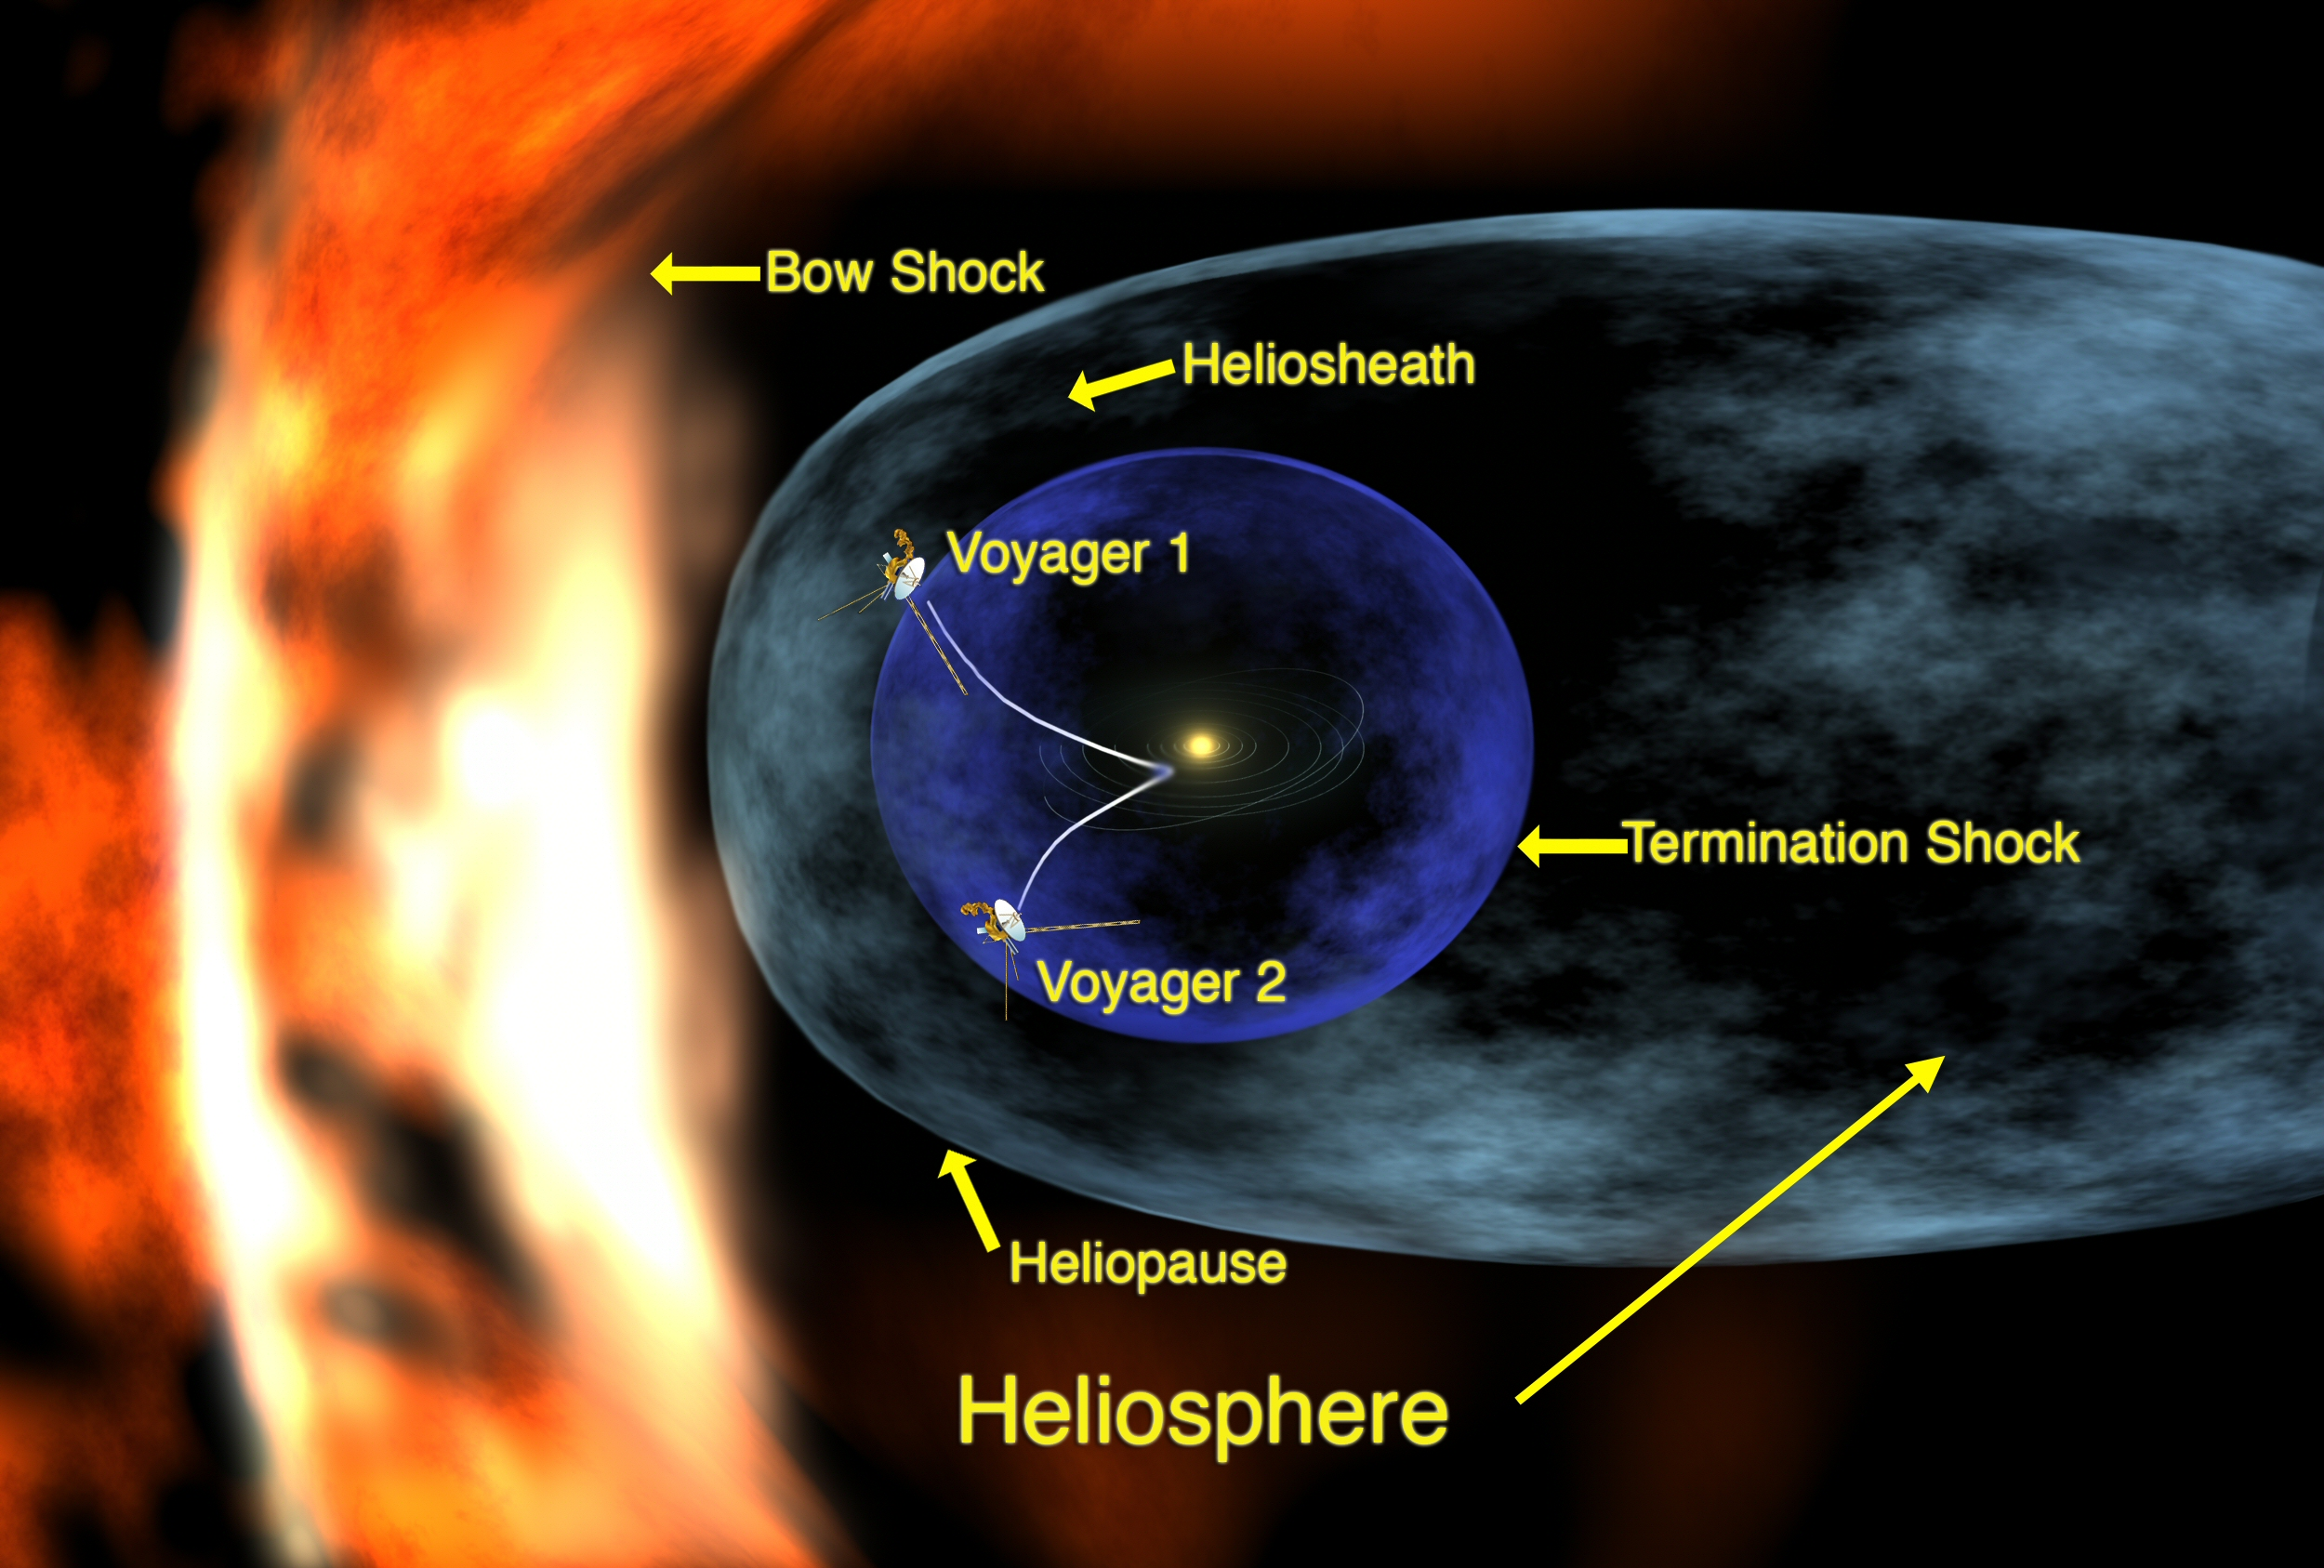
\includegraphics[width=0.43\textwidth,height=!]{./A/Voyager_1_entering_heliosheath_region.jpg}
\end{wrapfigure}  \vspace{0.1cm} The Solar wind blows out a cavity inside the
local ionised cloud (LIC). The heliosphere is about 100~AU in
diameter, with $N_e \sim 1 \times (1/ (r/\mathrm{AU})^2)~$cm$^{-3}$,
and $T_e \sim 10^4$~K. Optical absorption lines in the LIC have
$W_\lambda \sim 200$~m\AA, $b \sim$1~km~s$^{-1}$, and correspond to a
singly ionised gas with $T_e \sim 7000$~K, $N_e \sim 0.1$~cm$^{-3}$. 

\medskip

The LIC is embedded in the Local Bubble, $N_e \sim 5~10^{-3}$~cm$^{-3}$,
$T_e \sim 10^6~$K.

\medskip

Vallerga et al. (1993) show that the local ISM, the bulk of clouds
within the Local Bubble, is at rest in the LSR $\pm$11~km~s$^{-1}$ as
traced by CaII, and $\pm$3.6~km~s$^{-1}$ as traced by Na I. The solar
motion relative to the LSR is about 20~km~s$^{-1}$ in the direction of
Scorpius. 

\end{frame}

%\end{itemize}


\frame{\frametitle{Crude measures of the very local ISM density}



\begin{center}
%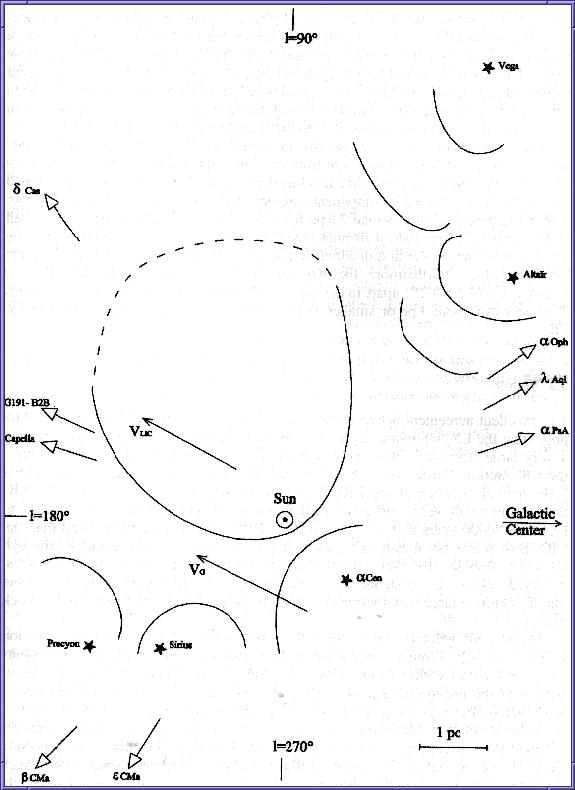
\includegraphics[width=!,height=0.7\figheight]{./A/localism_ferlet.jpg}
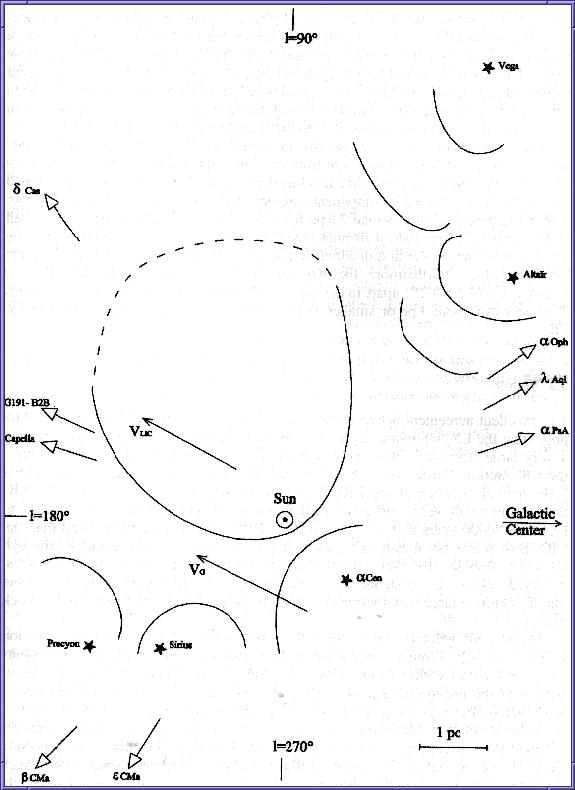
\includegraphics[width=!,height=\figheightscl]{./A/localism_ferlet.jpg}
%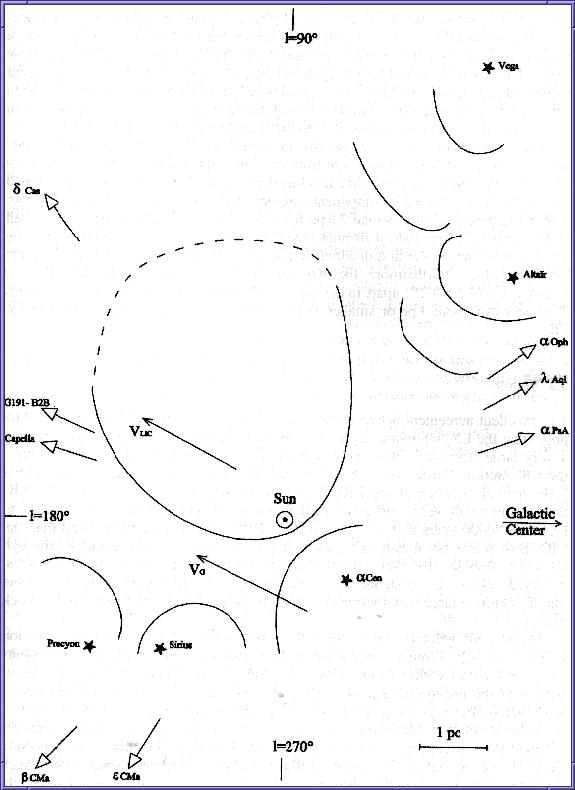
\includegraphics[width=!,height=1.0\figheight]{./A/localism_ferlet.jpg}
\end{center}
{\tt Ferlet 1999, A\&ARv, 9, 153}
%\citet{1999A&ARv...9..153F}


}

\subsection{The Local Bubble}

\frame{\frametitle{The Local Bubble.}

\begin{center}
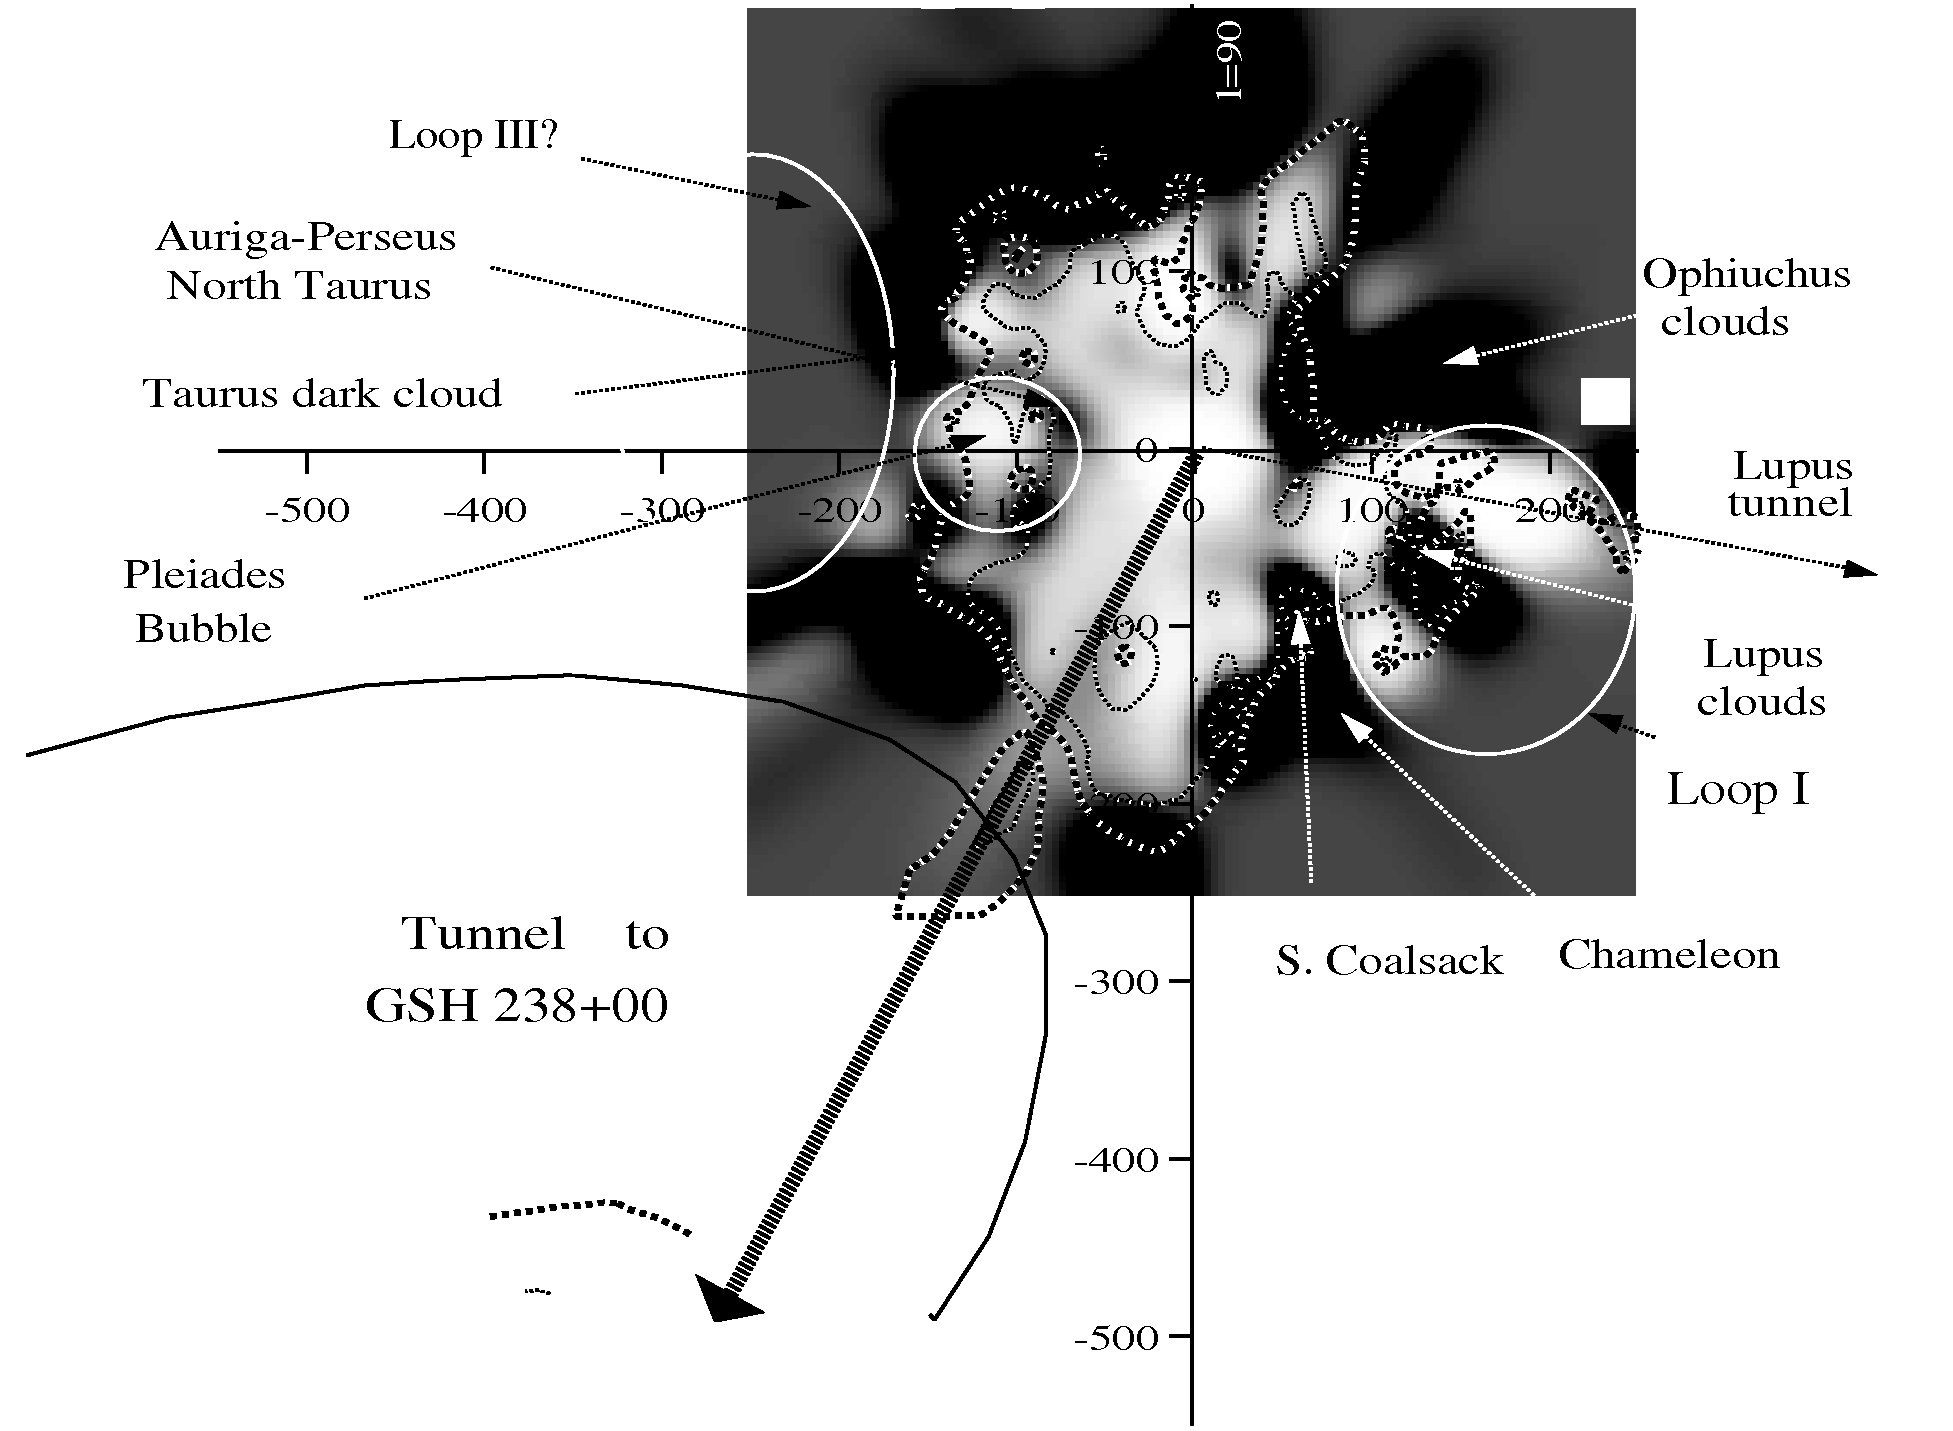
\includegraphics[width=0.9\textwidth,height=!]{./A/fig_lallement_fig1.jpg}
\end{center}
Na D lines maps. Contours at $W_\lambda =20~$m\AA~ and 50~m\AA~. Lallement et al. (2003, A\&A 411, 447).

}

\frame{

\frametitle{The Local Chimney}

\vspace{-0.5cm}
\begin{minipage}[t]{0.49\textwidth}
\vspace{+0.5cm}
\begin{center}
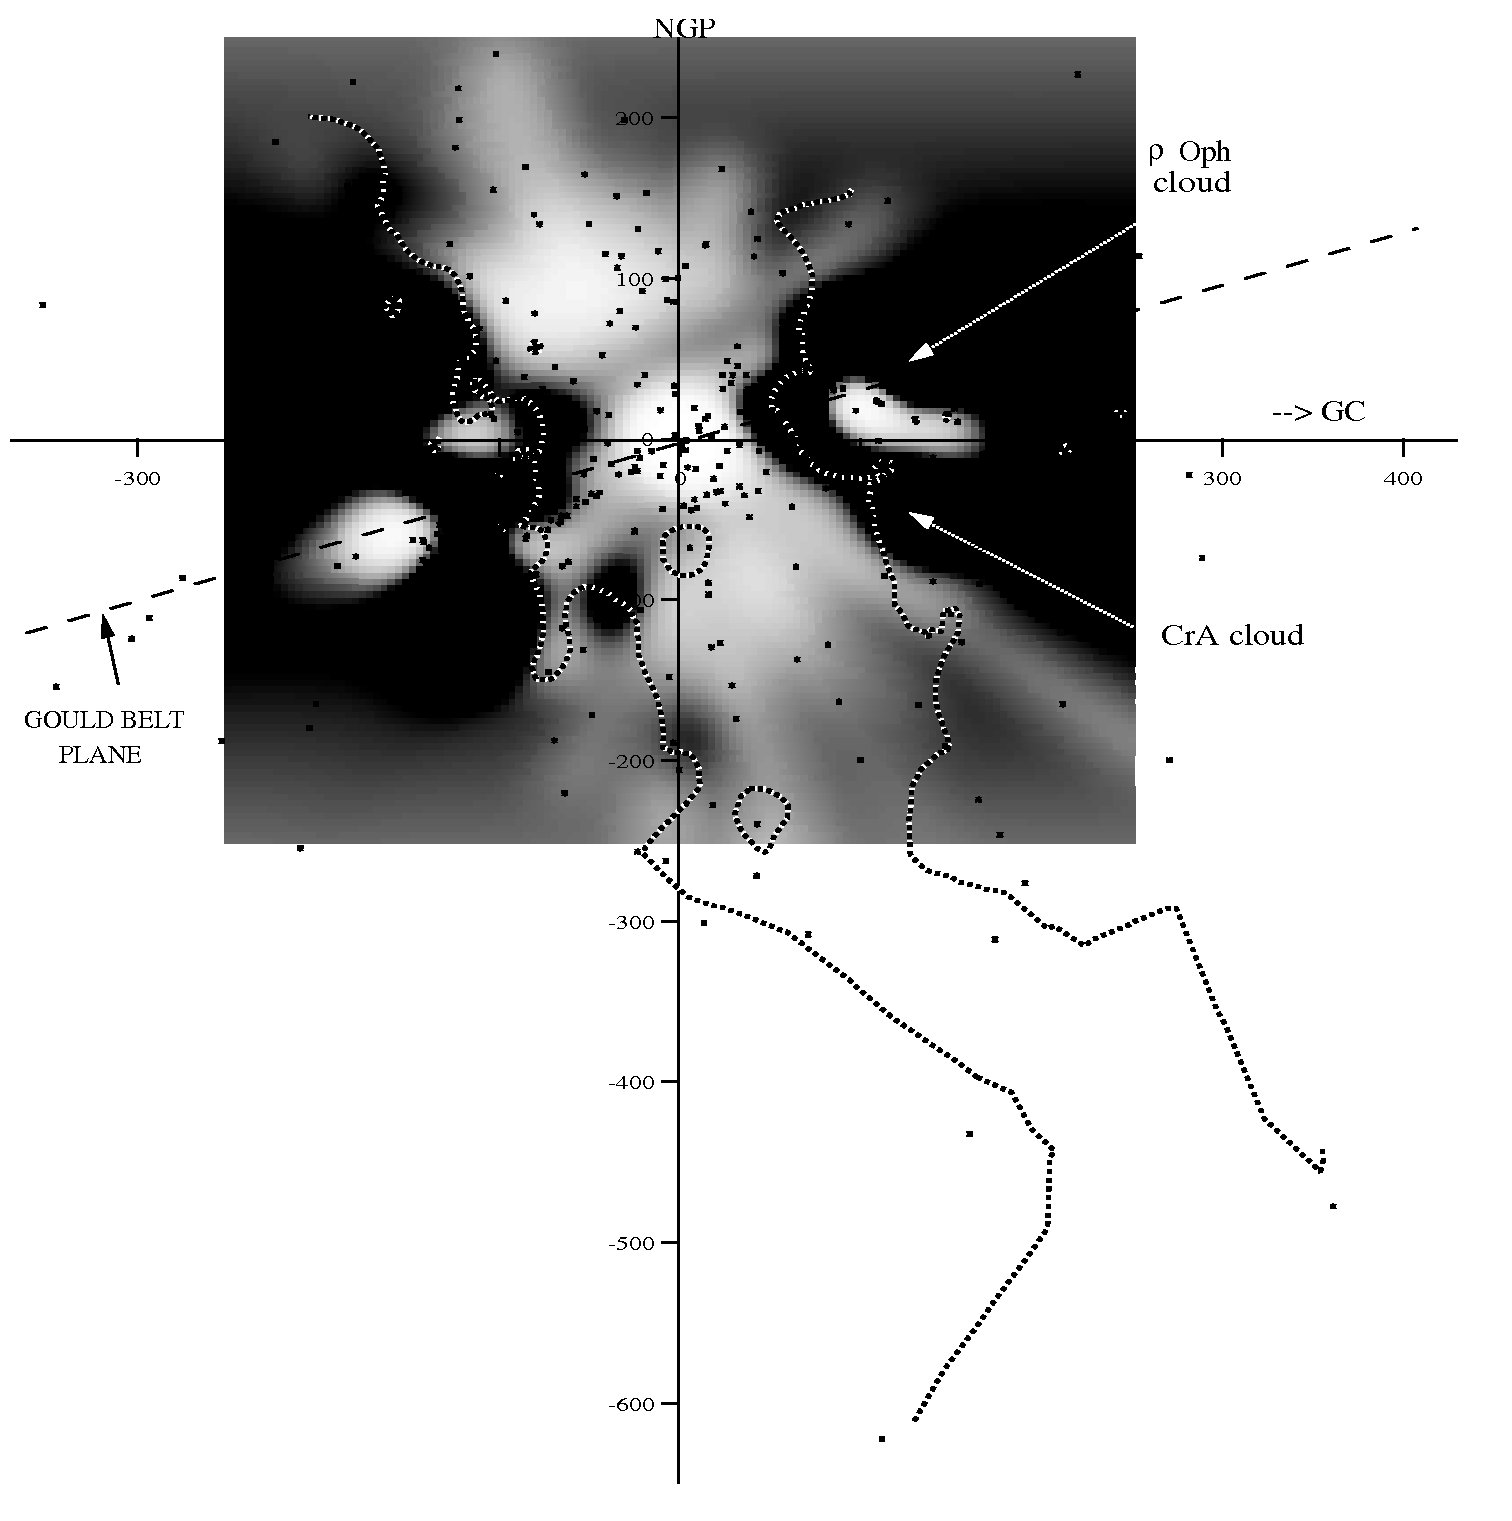
\includegraphics[width=\textwidth,height=!]{./A/fig_lallement_fig2.jpg}
\end{center}
\end{minipage}
\begin{minipage}[t]{0.49\textwidth}
\vspace{2cm}
\begin{itemize}
\item The Local Bubble appears to be squeezed into a Local Chimney by
SNR shells. The Local Chimney is very narrow: about 20~deg towards
each Galactic pole, corresponding to directions of minimal diffuse
H$\alpha$ and far-IR.
\end{itemize}
\end{minipage}
}

%\frame{\frametitle{The Local Chimney}
%
%%\vspace{-0.5cm}
%
%\begin{columns}[t,onlytextwidth]
%%\begin{columns}[t]
%
%\column{0.49\textwidth}
%
%\begin{center}
%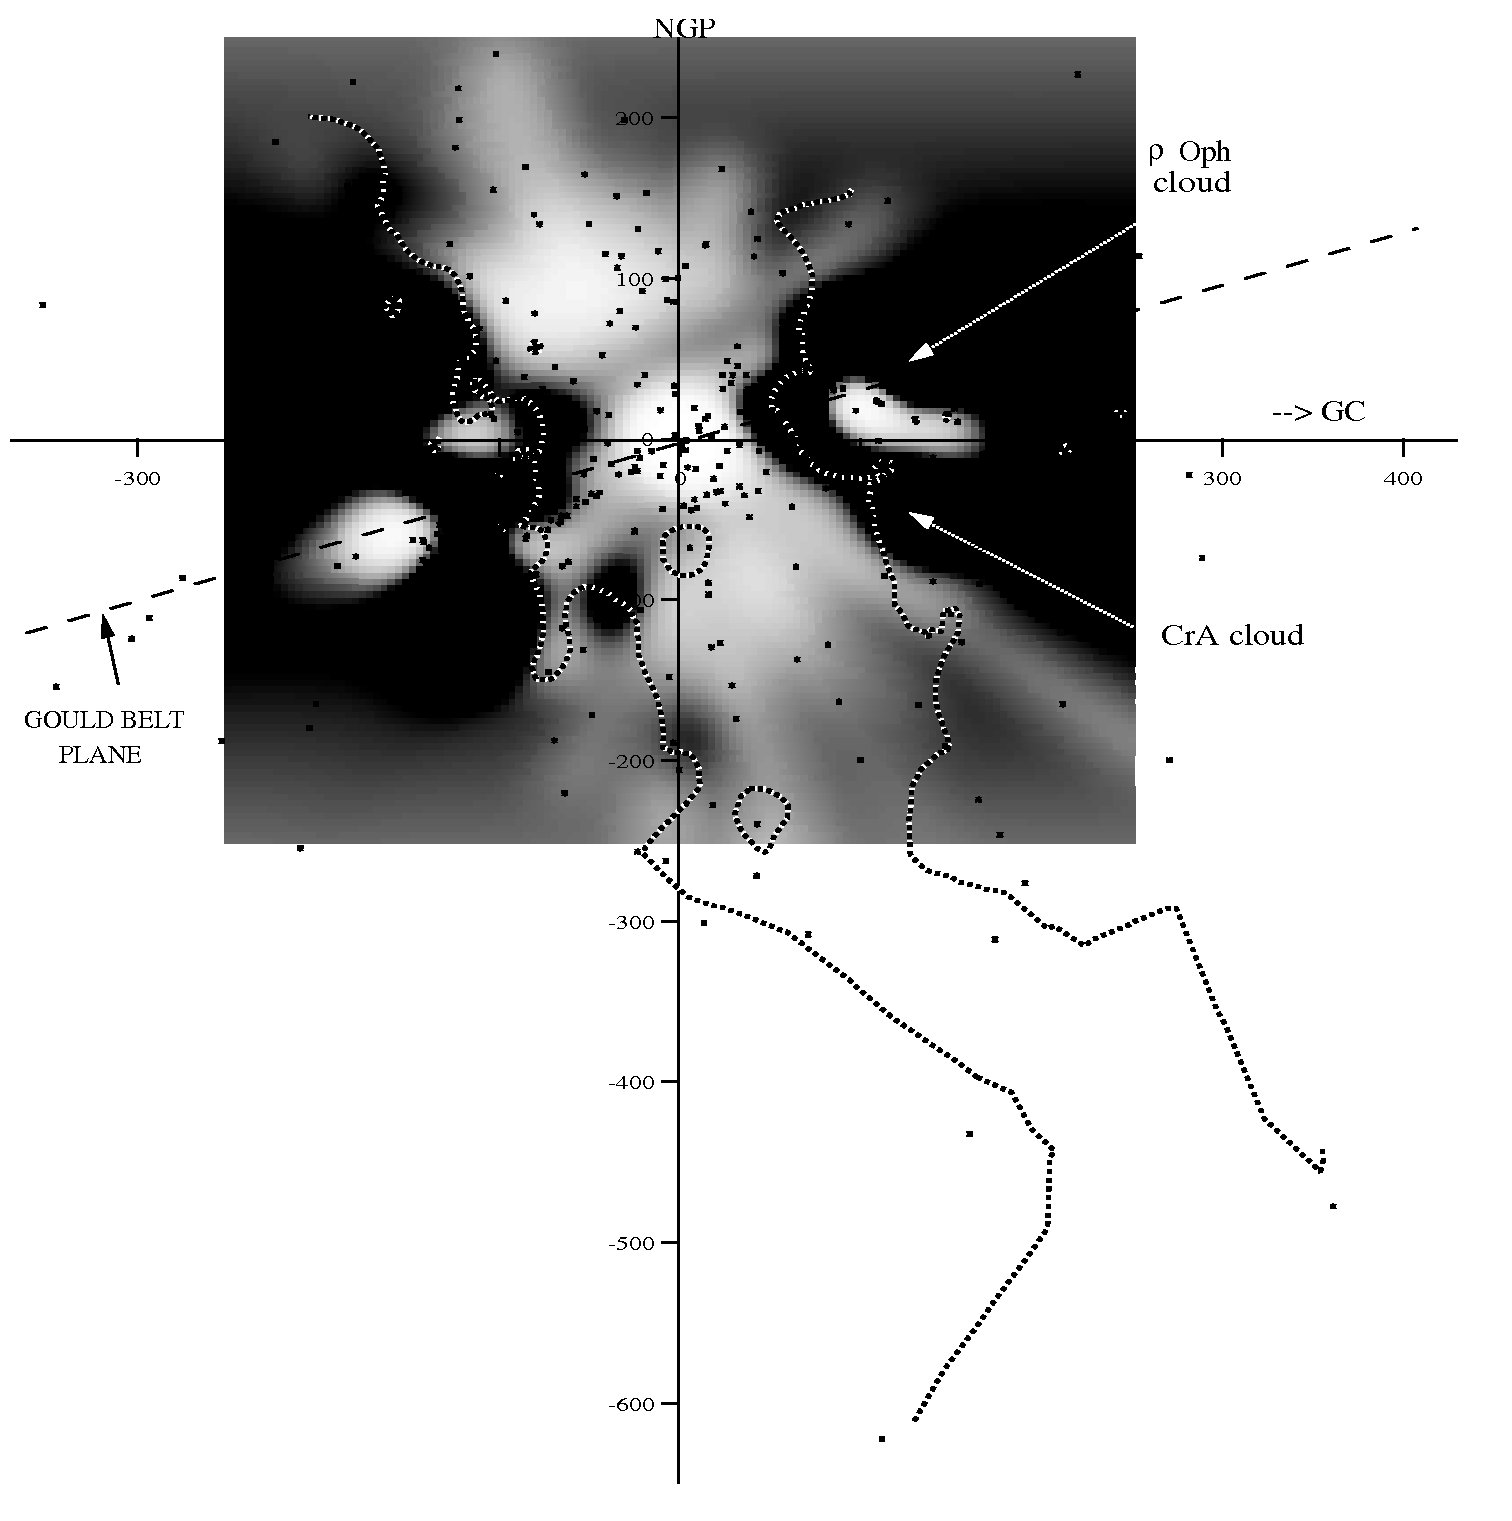
\includegraphics[width=\textwidth,height=!]{./A/fig_lallement_fig2.jpg}
%\end{center}
%
%\column{0.49\textwidth}
%
%The Local Bubble appears to be squeezed into a Local Chimney by
%SNR shells. The Local Chimney is very narrow: about 20~deg towards
%each Galactic pole, corresponding to directions of minimal diffuse
%H$\alpha$ and far-IR.
%\end{columns}
%
%
%}

\frame{\frametitle{Extragalactic windows}

Lallement et al. (2003) explain that ``no distinct and continuous
neutral boundary to the ends of the Local Chimney has been found in
either galactic hemisphere for distances $<$400~pc''. Crawford et
al. (2002) favor a picture of the inner galactic halo in which a
population of infalling IVCs lie along the Local Chimney. 

\medskip

{\large $\rightarrow$ The main absorbers in the local ISM towards
extragalactic objects are probably the boundaries of the Local
Chimney.}
}



\frame{\frametitle{Further 3D maps of the local ISM: face-on}
New density fields from Welsh, Lallement et al., 2010, A\&A, 510, A54


\begin{minipage}[t]{0.49\textwidth}
\begin{center}
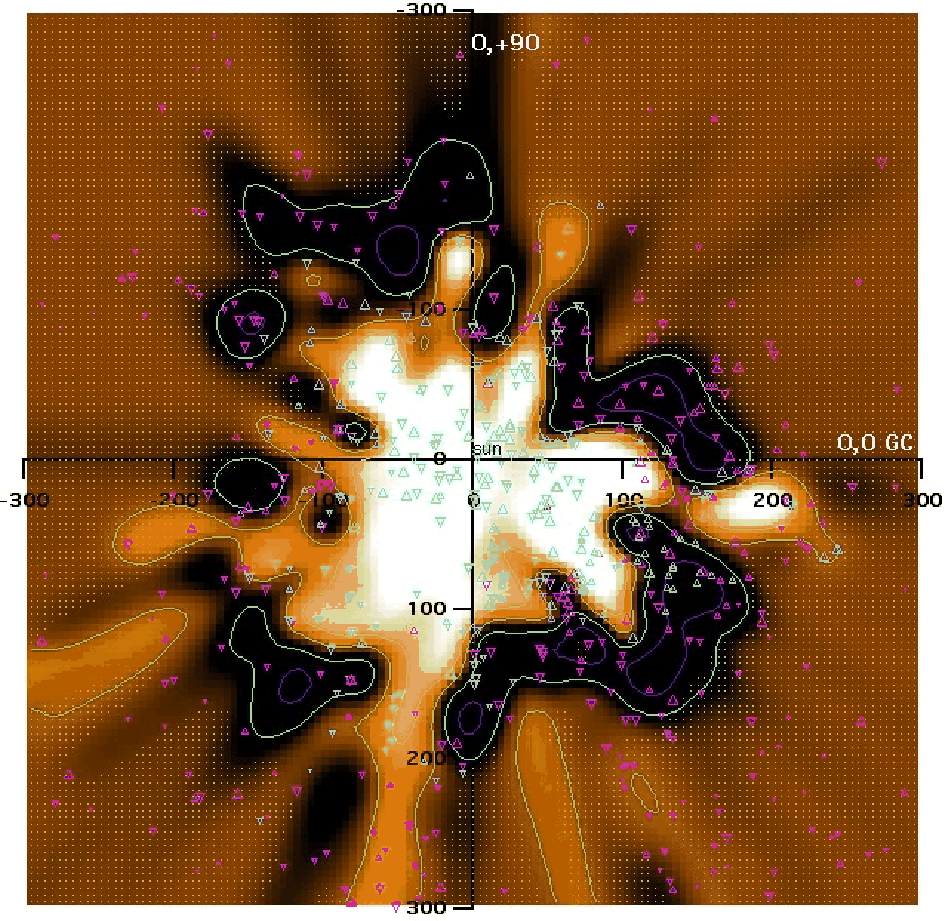
\includegraphics[width=\textwidth,height=!]{./A/welsh_fig12.png}

Na\,{\sc i} 
\end{center}
\end{minipage}
\begin{minipage}[t]{0.49\textwidth}
\begin{center}
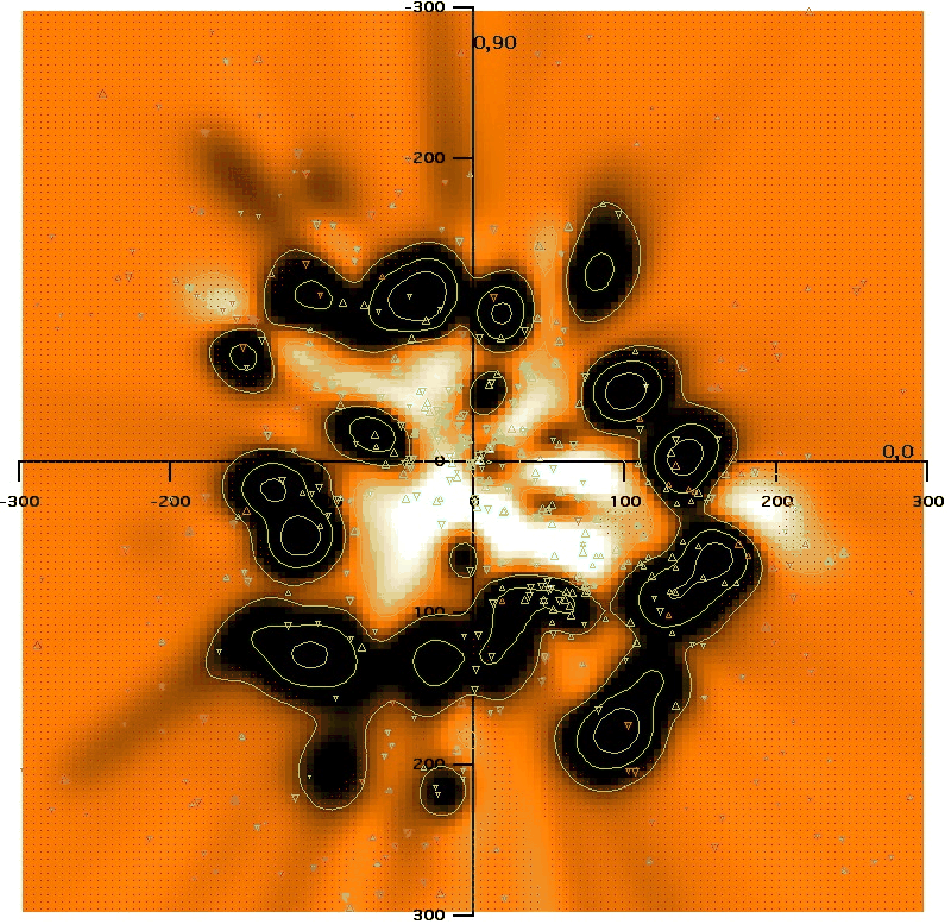
\includegraphics[width=\textwidth,height=!]{./A/welsh_fig15.png}

Ca\,{\sc ii}
\end{center}
\end{minipage}

}


\frame{ \frametitle{Further 3D maps of the local ISM: side view} 


\begin{minipage}[t]{0.49\textwidth}
\begin{center}
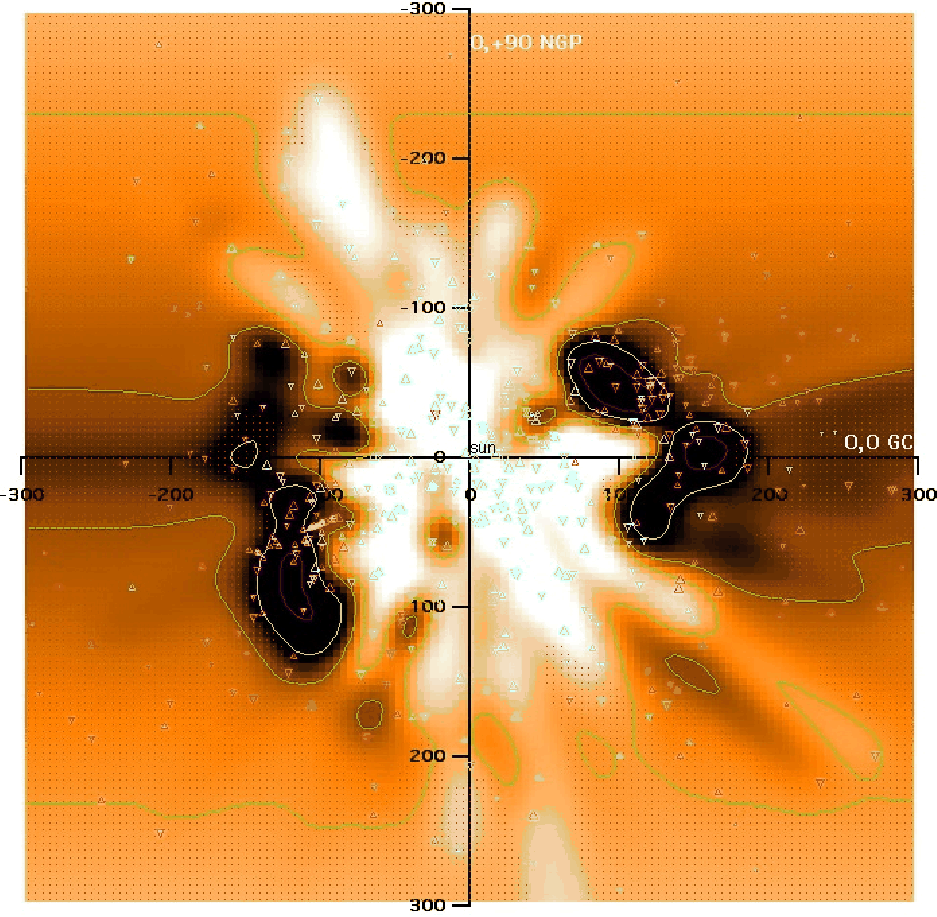
\includegraphics[width=\textwidth,height=!]{./A/welsh_fig13.png}

Na\,{\sc i} 
\end{center}
\end{minipage}
\begin{minipage}[t]{0.49\textwidth}
\begin{center}
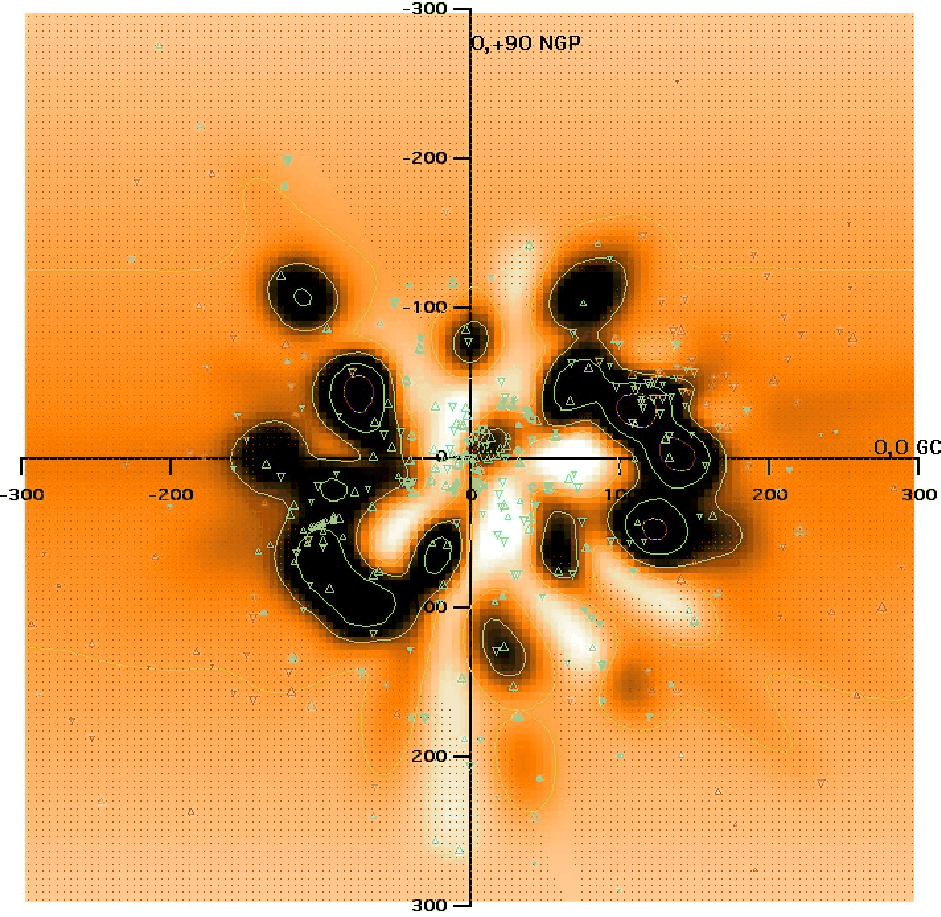
\includegraphics[width=\textwidth,height=!]{./A/welsh_fig16.png}

Ca\,{\sc ii}
\end{center}
\end{minipage}




}







\section{Morphology of interstellar clouds}

\subsection{Old model for clouds in thermal equilibrium}

\frame{\frametitle{Morphology of interstellar clouds}
%\hypersetup{pdfpagetransition=Dissolve}





Interstellar absorption lines (e.g.: CH$^{+}\lambda 4232$\AA,
CH$\lambda 4300$\AA, CN$\lambda 3875$\AA, etc..., ref: Dunham 1937,
PASP, 49, 26; Douglas \& Herzberg 1941, ApJ, 94, 381; Adams 1949,
ApJ, 109, 354) 

%\begin{minipage}[t]{11cm}
%\begin{center}
%\includegraphics[width=11cm,height=!]{fig_ZOPH.pdf}
%\end{center}
%\end{minipage}
%\hfill
%\begin{minipage}[t]{11cm}


%\footnote{S/N~2000, $\Delta~\lambda$~0.05\AA,
%(Casassus et al. 2004, in prep)}


\begin{center}
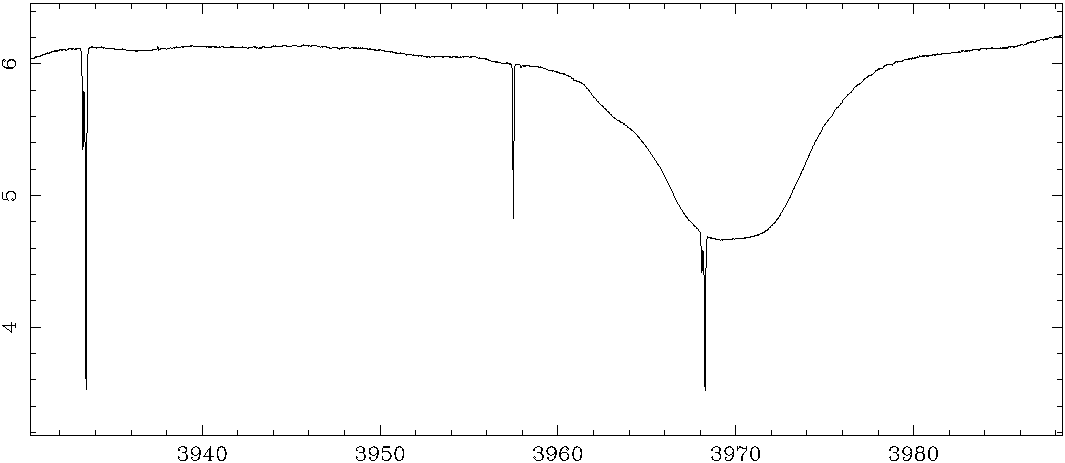
\includegraphics[width=0.7\textwidth,height=!]{./A/zetaOph_3960.pdf}\\
\mbox{$\zeta$Oph VLT+UVES spectrum around $\sim$3960\AA}
\end{center}


}


\frame{ \frametitle{Old model} 
\begin{center}
$\zeta$Oph VLT+UVES spectrum around  $\sim$3960\AA - zoom.
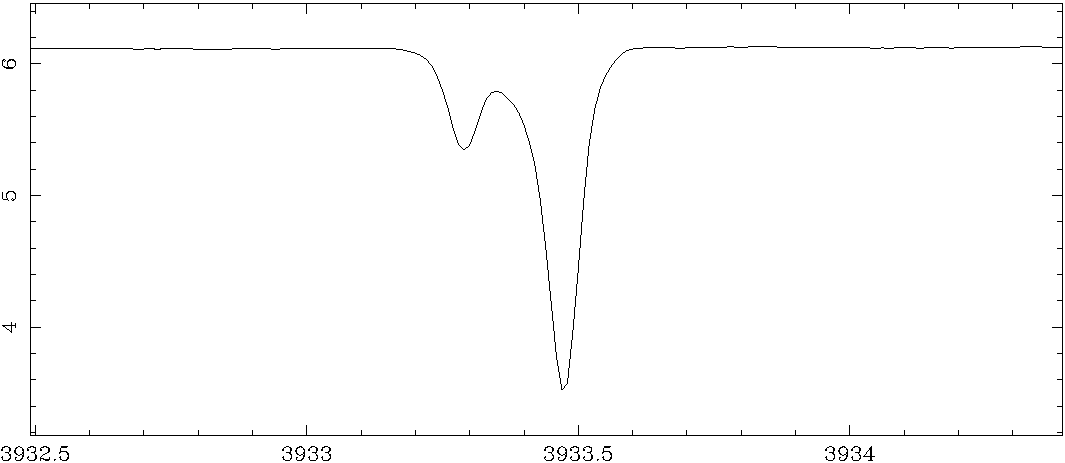
\includegraphics[width=0.7\textwidth,height=!]{./A/zetaOph_CaII3933.pdf}
\end{center}

$\rightarrow$ \\ model of discrete clouds confined
by pressure equilibrium with the the intercloud medium, $T\sim10^6$K
(e.g. Spitzer, 1956, ApJ, 124, 20), confirmed through the observation
of O{\sc~vi}$\lambda$1031 absorption towards nearby stars ({\em
Copernicus}$\sim$1973, {\em FUSE} $\sim$2002).

}

\subsection{Realistic descriptions}

\frame{ \frametitle{Problems with the discrete cloud model}

(Elmegreen \& Falgarone, 1996, ApJ, 471, 816)
\begin{itemize}
\item Supersonic motions imply that the dynamics of the clouds are
dominated by shocks, not thermal pressure.
\item Improving the angular resolution of interstellar cloud maps
invariably result in the discovery of substructure.
\item Linear size, mass, and velocity dispersion are related by power
laws, which can be characterised through scaling laws: \( N(L) \propto
M(L) \propto L^{D}.  \) Power laws are typical of self-similar
structures. A function  $y=f(x)$ whose properties only change by a
factor $b$ when applying a scaling factor $a \times x$ must fulfill 
\( f(a\,x) = b f(x) \). Scaling $k$ times,   $x = a^k x_\circ $, and $y =
b^k y_\circ$, from which $y = x^c$, with $c = \ln(b)/\ln(a)$. If $y$
is the number of structures or the mass, and if $x$ is size, then $c$
is the fractal dimension of the selfsimilar structure. 

\end{itemize}

\vfill

}
\begin{frame} \frametitle{Morphology of the  ISM: scaling laws} 

\begin{center}
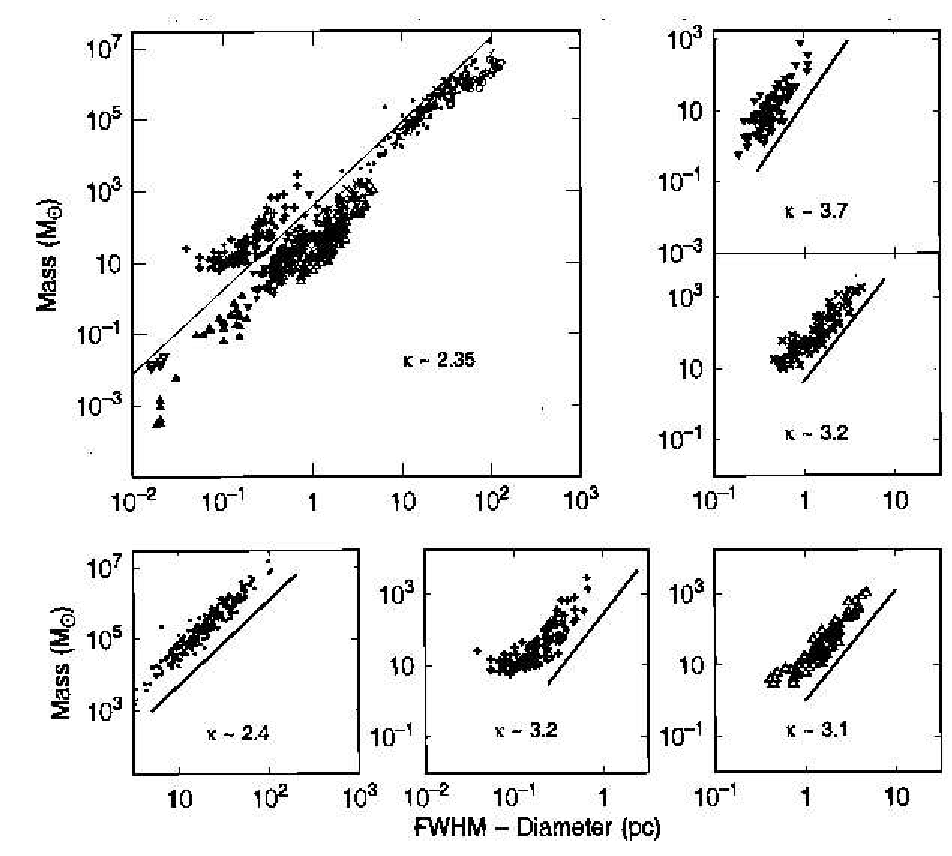
\includegraphics[width=\textwidth,height=!]{./A/ml.pdf}
\end{center}



\end{frame}

\begin{frame}{Morphology of the ISM: Armonic analysis} 

The structure of the ISM can also be described by an armonic analysis,
with the power spectrum of the specific intensity maps: \( P(k)
\propto k^{\alpha} \), in which  $P(k)$ is the modulus of  \( F(k) = \int
dxdy I(x,y) \exp(2i\pi
\vec{k}.\vec{x}), \) with an angle average for isotropic
distributions. The power spectrum allows the inference of basic
properties of the emission maps, such as characteristic angular sizes,
relative importance of angular scales, etc....  \\

For scales larger than $>$10~deg, it is necessary to take into account
the curvature of the celestial sphere:
\[I(\hat{r},\nu) = \sum_l\sum_m Y_{lm}(\hat{r}) a_{lm}(\nu),
\] and the power spectrum is 
\(
C_l \equiv 1/(2l+1) \sum_{m=-l}^{m=+l} \langle
\|a_{lm}(\nu)\|^2 \rangle 
\), in the definition by  Tegmark \& Efstathiou, 1996, MNRAS, 281,
1297.  In a flat aproximation to the celestial sphere, $k =
(l+1/2)/2\pi$, and $k^2P(k) = l (l+1) C_l / (2\pi)^2$, with $k$ in
rad$^{-1}$.

\end{frame}

\frame{\frametitle{Example power spectra} 

\begin{itemize}
\item CMB. 
\item white noise, with  $P(k) = $~Cte.  Example: point sources with a
random distribution (i.e. Poisson). On average,
\(
\langle a_{lm} \rangle = \int d\Omega  ~Y^{\star}_{lm}(\Omega) \langle
  I(\hat{r})\rangle,
\) with  $\langle I(\hat{r})\rangle = \frac{N}{4\pi} \phi$, where $\phi$ 
  is the average flux density of $N$ sources in the sky. $\langle n
  \rangle = N/4\pi$ follows a Poisson distribution: $\langle n^2
  \rangle - \langle n \rangle^2 = \langle n \rangle$.
\(
\langle \| a_{lm} \|^2 \rangle = \int d\Omega d\Omega^\prime
 ~  Y^{\star}_{lm}(\Omega)  Y_{lm}(\Omega^\prime) ~ \langle
  I(\Omega)  I(\Omega^\prime)) \rangle,
\)\\ and as   \( \langle
  I(\Omega)  I(\Omega^\prime) \rangle = \delta(\Omega-\Omega^\prime)
  \phi^2 \langle n \rangle\)  \( \Rightarrow C_l = \phi^2 \langle n
  \rangle.\)  



\item power spectrum of the  {\em IRAS} syrvey. 
Ref: Gautier et al. (1992, AJ, 102, 1313), Miville-Desch\^eches et
al. (2007, A\&A, 469, 595):
$P(k) \propto k^{-2.9}$.
\item Recent analysis by  Oliveira-Costa et al. (2002, ApJ, 567,
  363). 
\end{itemize}

\vfill


}
\frame{\frametitle{ISM power spectra}  


\begin{center}
  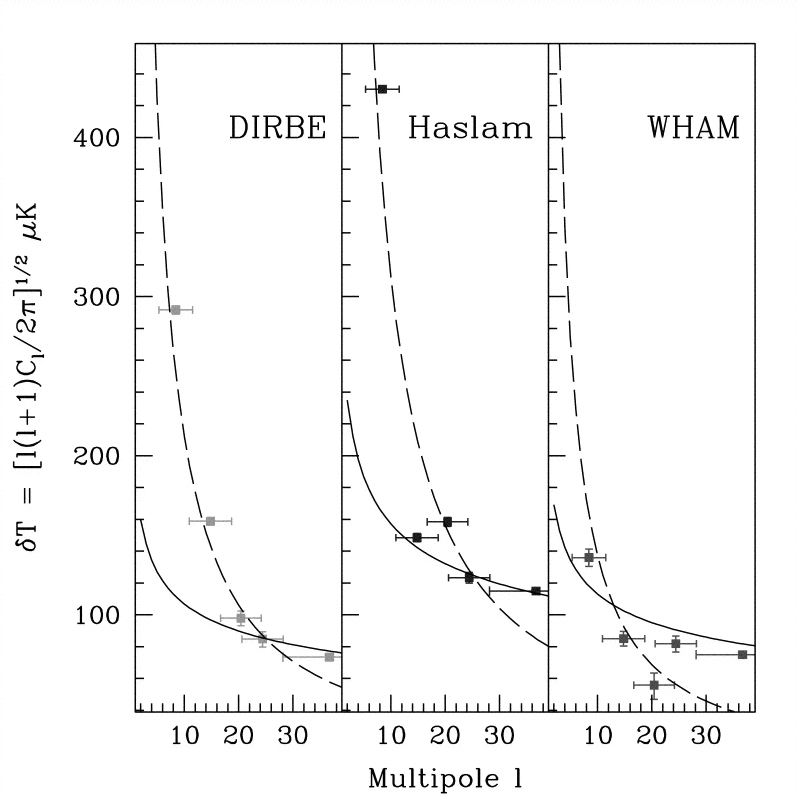
\includegraphics[width=0.49\textwidth,height=!]{./A/fg2.png}
  %{\tiny From \href{http://klab.agsci.colostate.edu/aegypti/aegypti.html}
  %{http://klab.agsci.colostate.edu/aegypti/aegypti.html}}
\end{center}

\vfill

}

\frame{ \frametitle{Morphology of the ISM: armonic analysis} 



\begin{minipage}[t]{0.49\textwidth}
\begin{center}
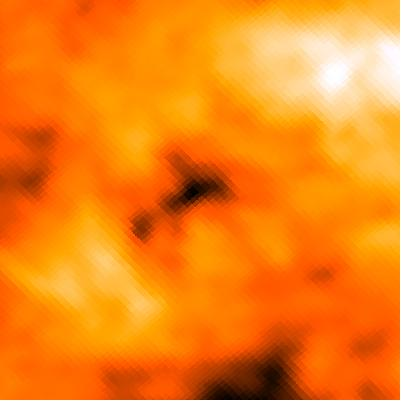
\includegraphics[width=\textwidth,height=!]{./A/zoph_sfd_3deg.jpg}
\end{center}
\end{minipage}
\begin{minipage}[t]{0.49\textwidth}
\begin{center}
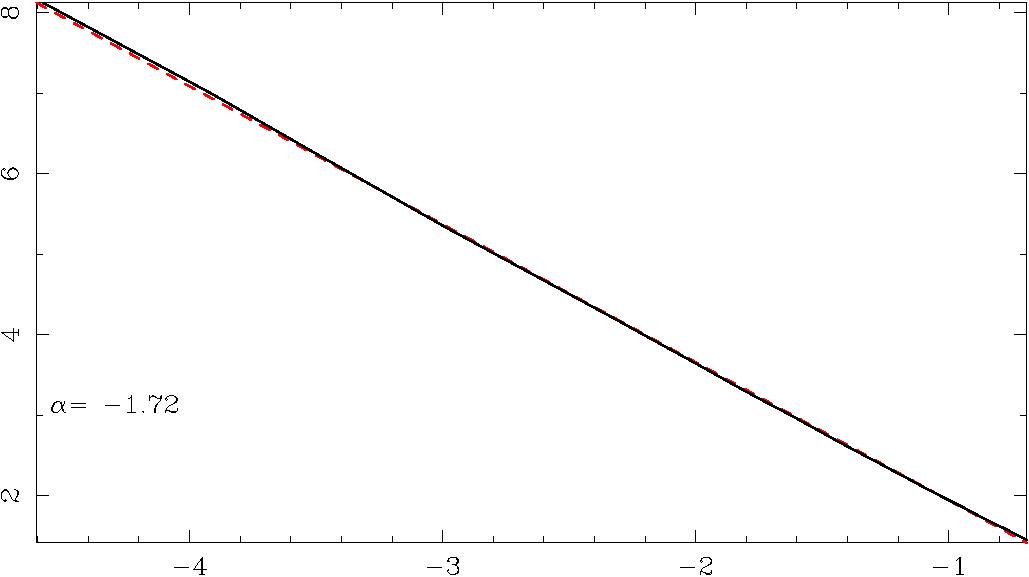
\includegraphics[width=\textwidth,height=!]{./A/sfdpowerspec.pdf}
\end{center}
\end{minipage}




\vfill

}

\frame{ \frametitle{Morphology of the ISM: relationship   between scaling laws and the power spectrum}

A self similar structure with a self-similar exponent $H$ has a 1-D
power spectrum $P(k) = \mathrm{Cte}~ k^{-1-2\,H}$ (e.g.  ``Fractals, a
User's Guide for the Natural Sciences'', Hastin \& Sugihara, 1993,
Oxford Science Publications).  \\

\medskip

A recipe for simulating fractals is therefore to generate a
power-spectrum whose amplitude has a variance of $k^{-1-2\,H},$ and
with random phases. Passing to the celestial plane and taking real
parts, one gets a self-similar structure with fractal dimension
$2\,H$, and with random phases. Switching to the image plane and
taking real parts one obtains a self-similar structure with fractal
dimension $2\,H$, and with random phases. The requisite $P(\hat{k}) =
P^{\star}(-\hat{k})$ generates a real map.

}

\frame{ \frametitle{Morphology of the ISM: examples} 

Fractal analysis of an H\,{\sc i}~21~cm in the LMC (Elmegreen, Kim,
Staveley-Smith ,2001,ApJ,548,749)x.

\begin{center}
  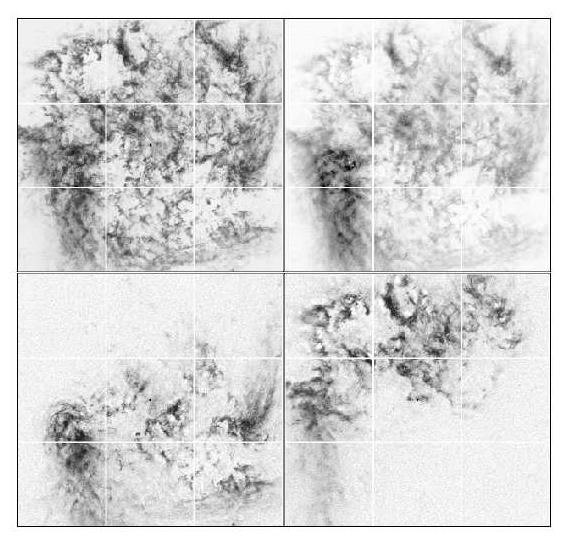
\includegraphics[width=0.7\textwidth,height=!]{./A/elemegreen_lmc_example_fig1_clip}
\end{center}

\vfill
}
\frame{ \frametitle{Morphology of the ISM: examples} 




\begin{minipage}[t]{0.49\textwidth}
\begin{center}
    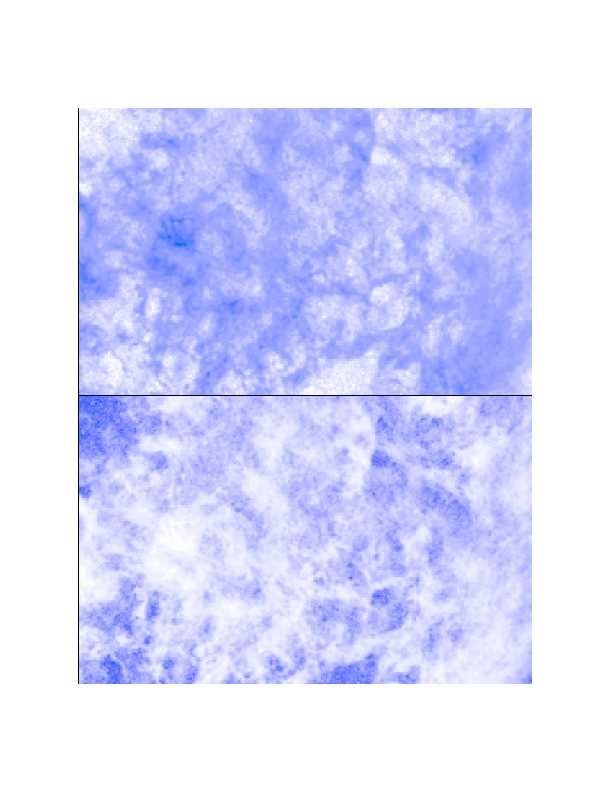
\includegraphics[width=\textwidth,height=!]{./A/elmegreen_lmc_example_fig10}
\end{center}
\end{minipage}
\begin{minipage}[t]{0.49\textwidth}
\begin{center}
    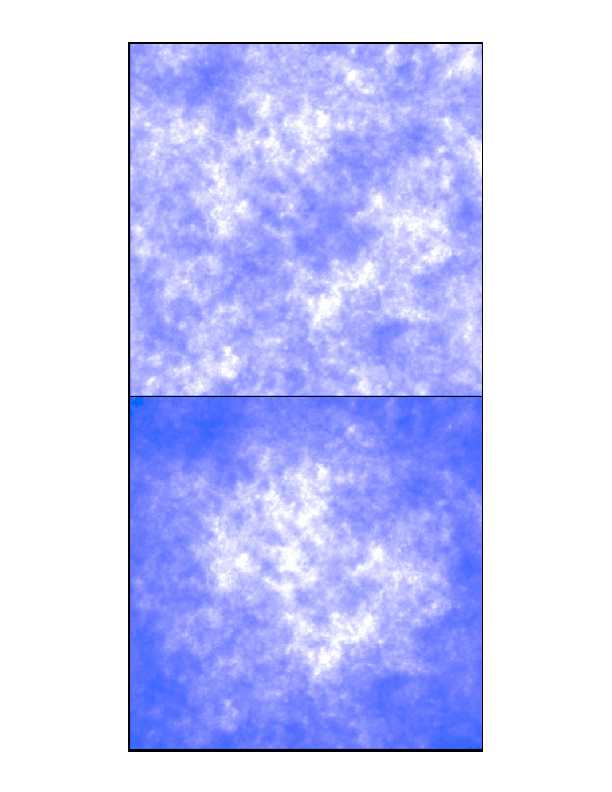
\includegraphics[width=\textwidth,height=!]{./A/elmegreen_lmc_example_fig15}
\end{center}
\end{minipage}



}

\section{Phases of the ISM}

\frame{\frametitle{Phases of the ISM} 

Molecular components (H$_2$), atomic (H\,{\sc i}, photo-dissociation
regions, or PDRs), ionised (H\,{\sc ii} regions, with T~10$^4$~K), and
hot plasma, with $T~10^6$~K.

\begin{center}
  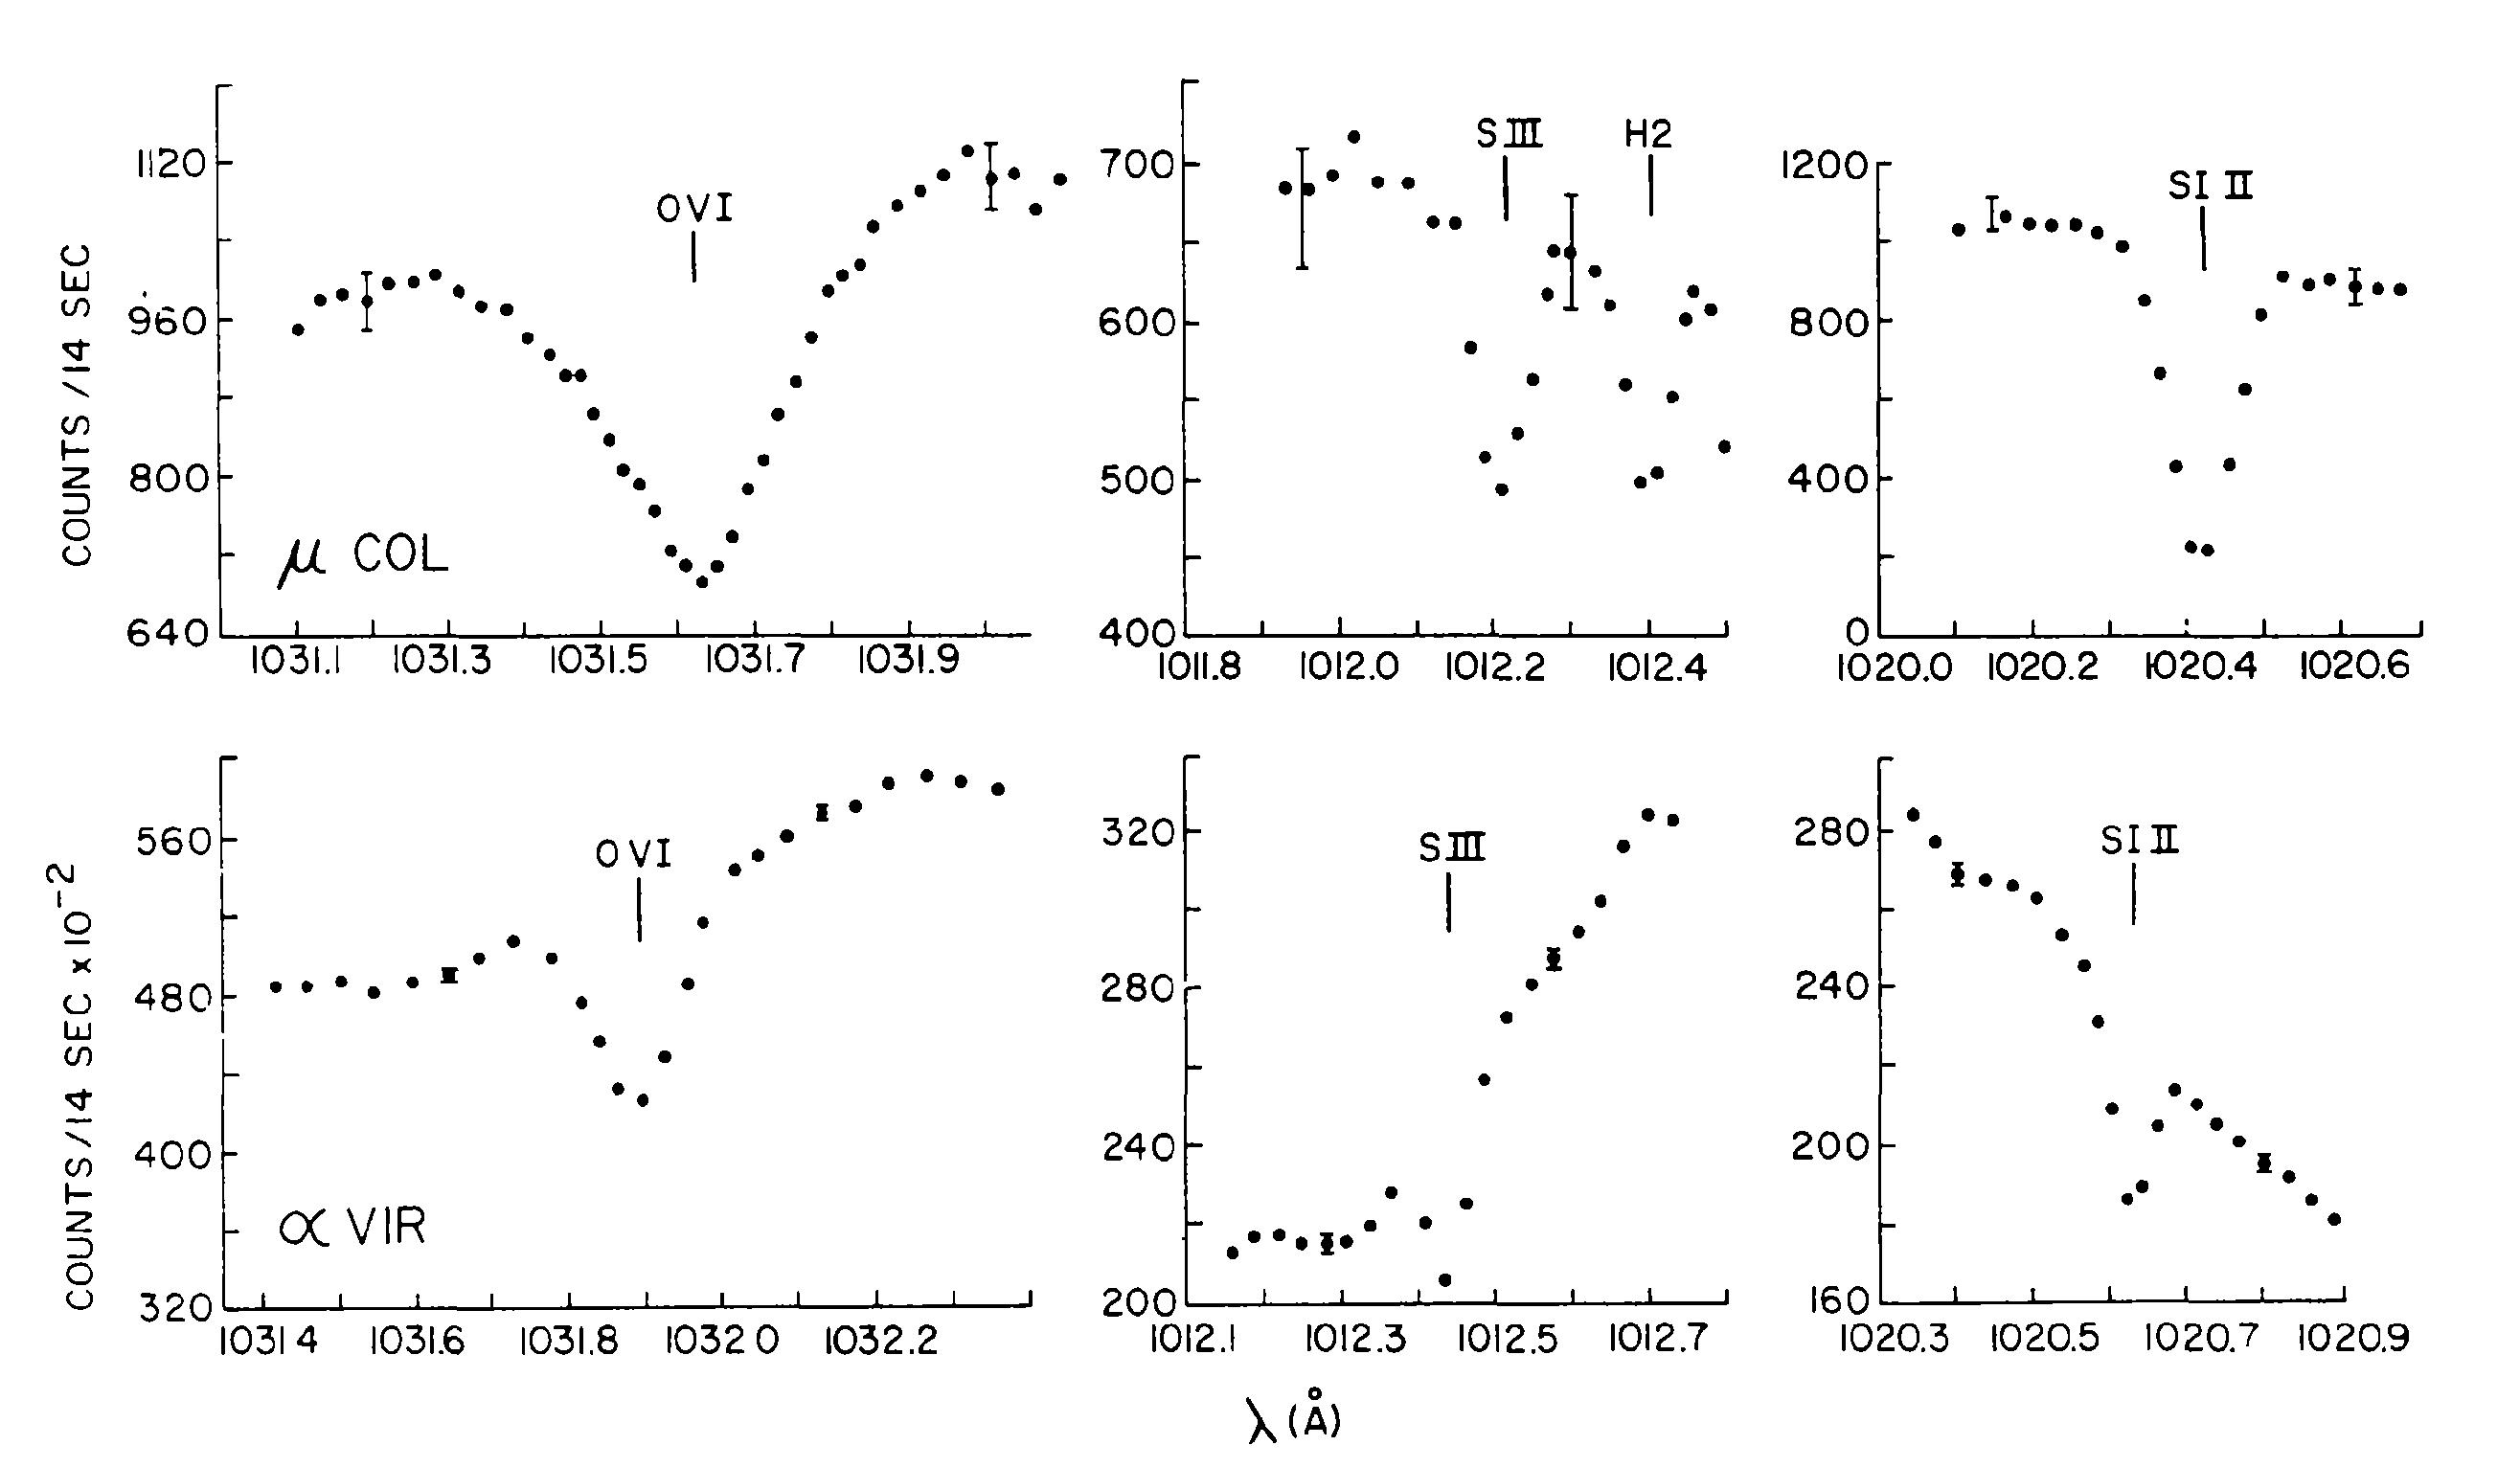
\includegraphics[width=\textwidth,height=!]{./A/york1974_ovi.jpg}
  %{\tiny From \href{http://klab.agsci.colostate.edu/aegypti/aegypti.html}
  %{http://klab.agsci.colostate.edu/aegypti/aegypti.html}}
\end{center}
\vfill

}

\frame{ \frametitle{Phases of the interstellar medium:
  dust in the H\,{\sc~i} region }



Depletion pattern in the neutral phase of the ISM towards  $\zeta$Oph
$\rightarrow$ dust at  18~K. 

\begin{minipage}[t]{0.4\textwidth}
\begin{center}
  
\includegraphics[width=\textwidth,height=!]{./A/zoph_sfd.jpg}
  {\tiny  {\tt http://skyview.gsfc.nasa.gov} }
\end{center}
\end{minipage}
\hfill
\begin{minipage}[t]{0.55\textwidth}
\begin{center}
 \rotatebox{-90}{ 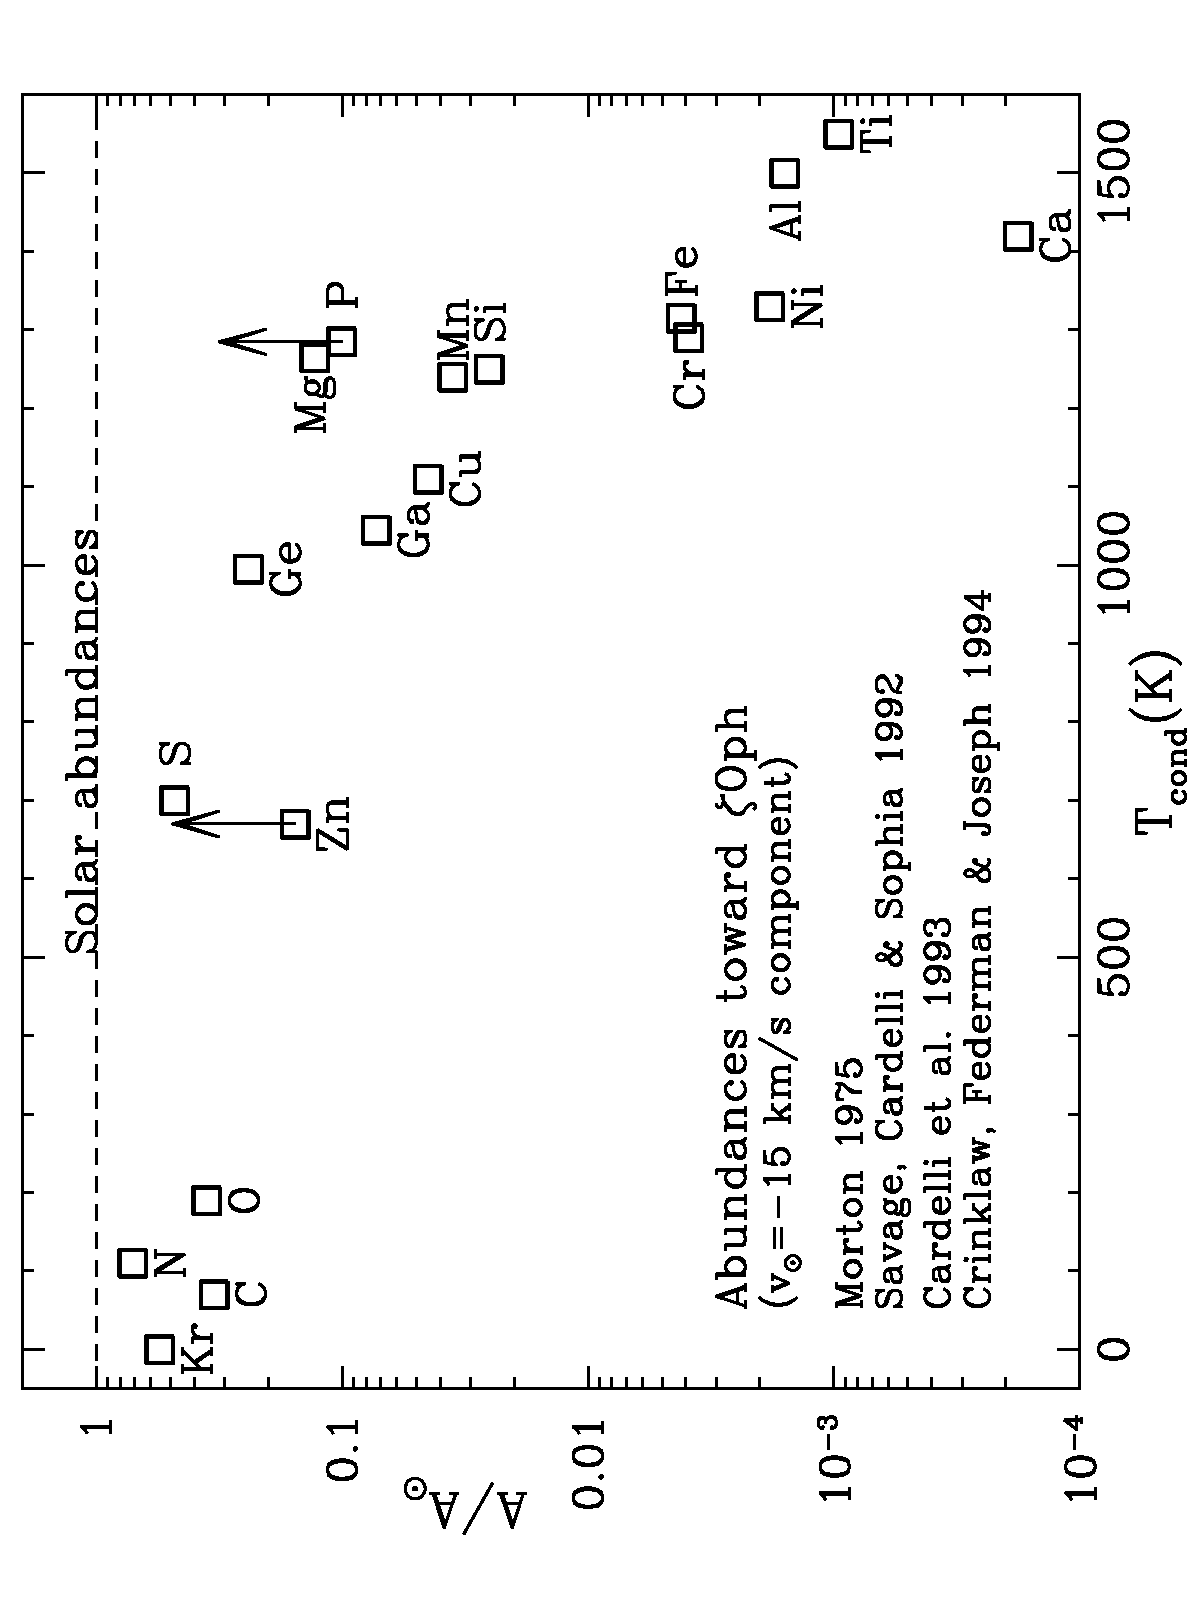
\includegraphics[width=0.6\textwidth,height=!]{./A/zoph_depletion.pdf}}
  %{\tiny From \href{http://klab.agsci.colostate.edu/aegypti/aegypti.html}
  %{http://klab.agsci.colostate.edu/aegypti/aegypti.html}}
\end{center}
\end{minipage}


}

\section{Mixing in the ISM}

\frame{  \frametitle{Mixing in the ISM} 

\begin{minipage}[t]{0.59\textwidth}
The isotopic ratio  $^{12}$C/$^{13}$C is a good tracer of the stellar
processing of the ISM. \medskip
%\vspace{-5cm}
\begin{center}
    \includegraphics[width=\textwidth,height=!]{./A/fig_ZOPH.pdf}

    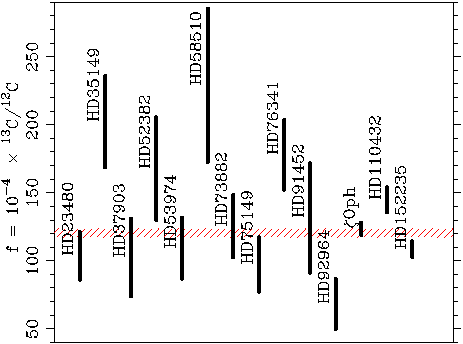
\includegraphics[width=0.6\textwidth,height=!]{./A/fig_all.pdf}

  \end{center}
\end{minipage}
\hfill
\begin{minipage}[t]{0.39\textwidth}
\vspace{0.1cm}
  \begin{center}
    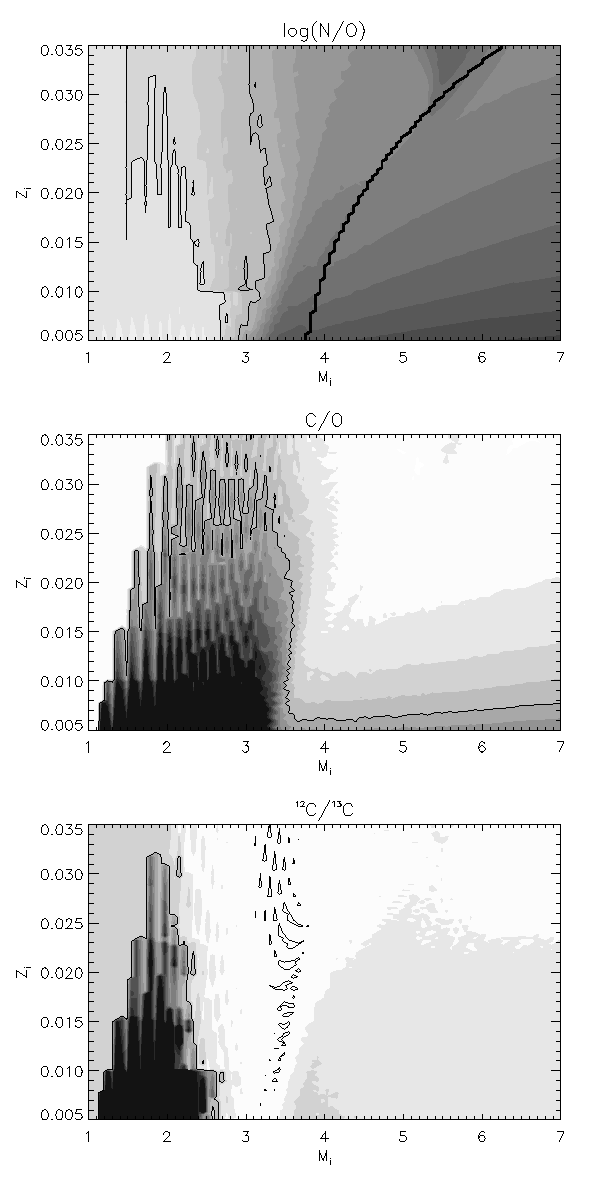
\includegraphics[width=\textwidth,height=!]{./A/mz.pdf}   
  \end{center}
\end{minipage}
\vfill



}

\section{Emission mechanisms  in the  ISM}

\frame{ \frametitle{Emission mechanisms in the ISM - synchrotron}
{\tt http://lambda.gsfc.nasa.gov/product/map/} \\
\begin{center}
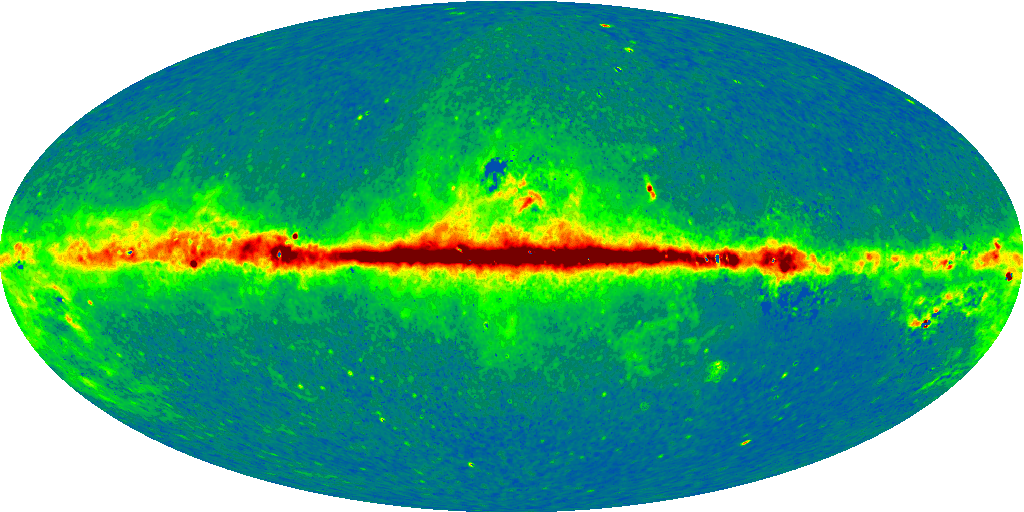
\includegraphics[width=\textwidth,height=!]{./A/lrg_mem_synch}
\end{center}
}

\frame{\frametitle{Emission mechanisms  - free-free}
\begin{center}
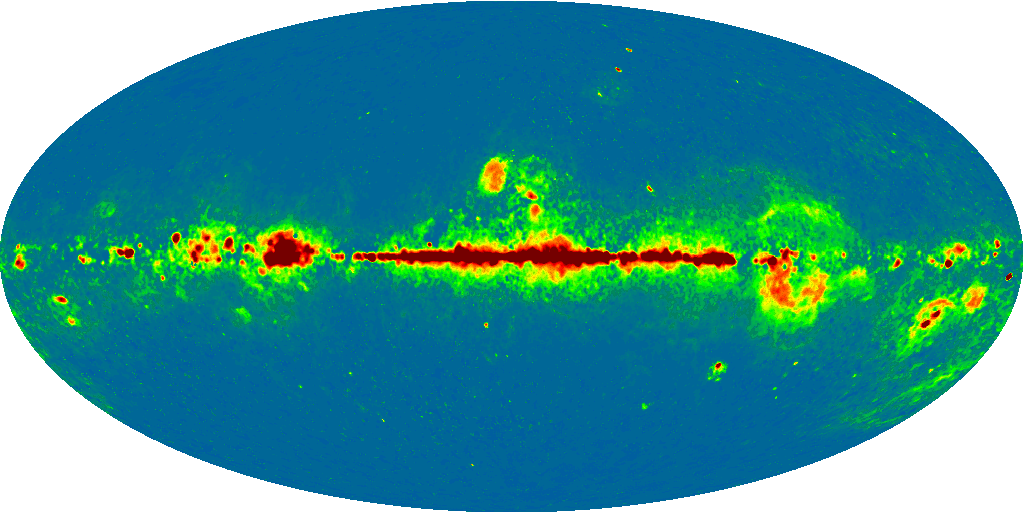
\includegraphics[width=\textwidth,height=!]{./A/lrg_mem_ff}
\end{center}
}

\frame{\frametitle{Emission mechanisms  - standard dust}
\begin{center}
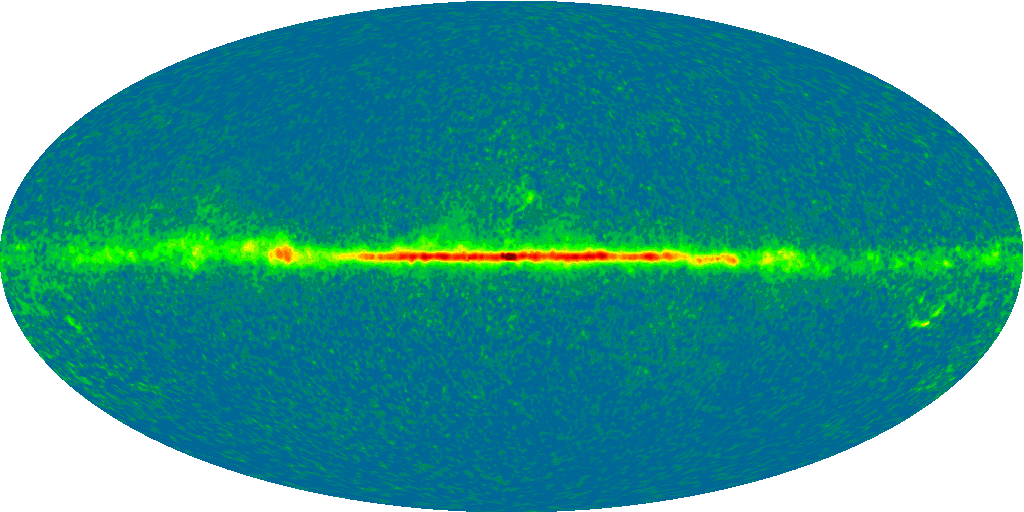
\includegraphics[width=\textwidth,height=!]{./A/lrg_mem_dust}
\end{center}
}

\section{Conspicuous features}

\frame{\frametitle{Conspicuous features}
\begin{center}
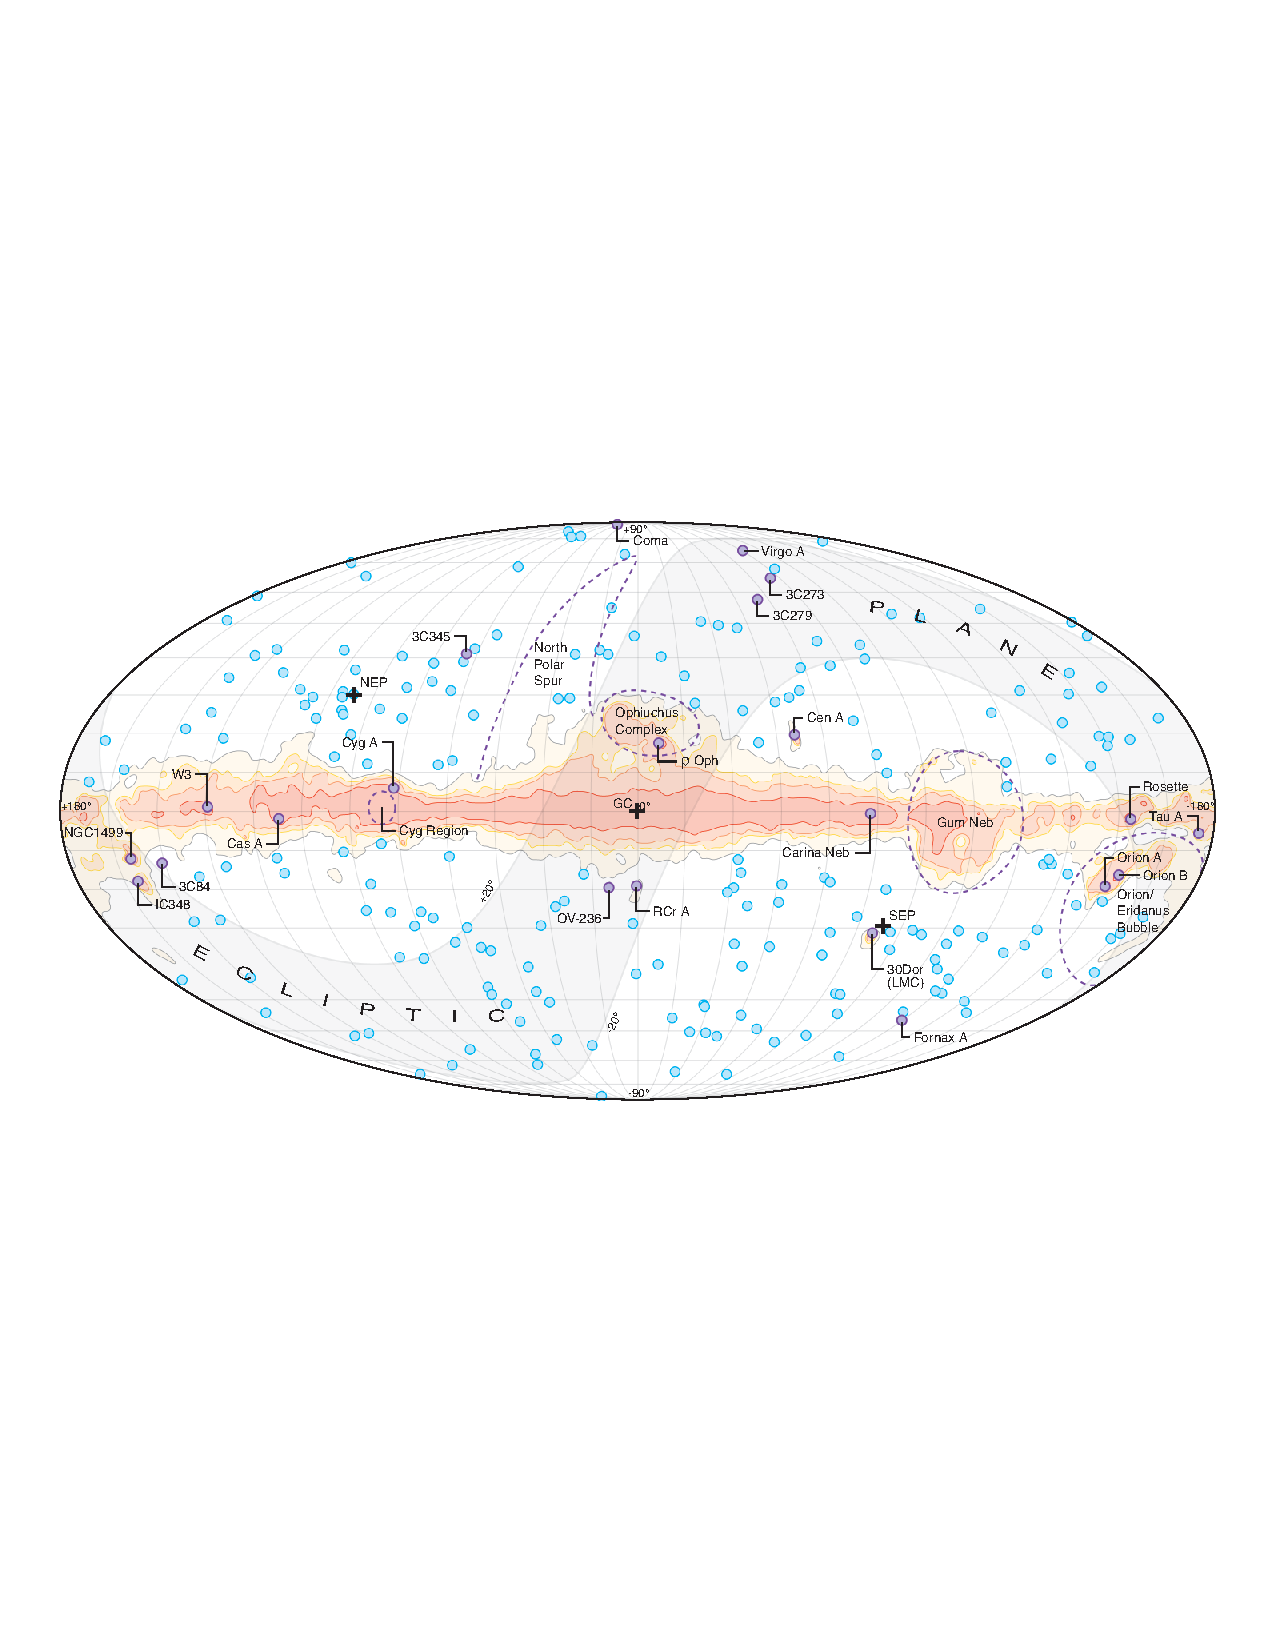
\includegraphics[width=\textwidth,height=!]{./A/wmap_expl}
\end{center}
}


\frame{ \frametitle{Conspicuous features - Planck} 

{\tt http://www.esa.int/SPECIALS/Planck/index.html}
\begin{center}
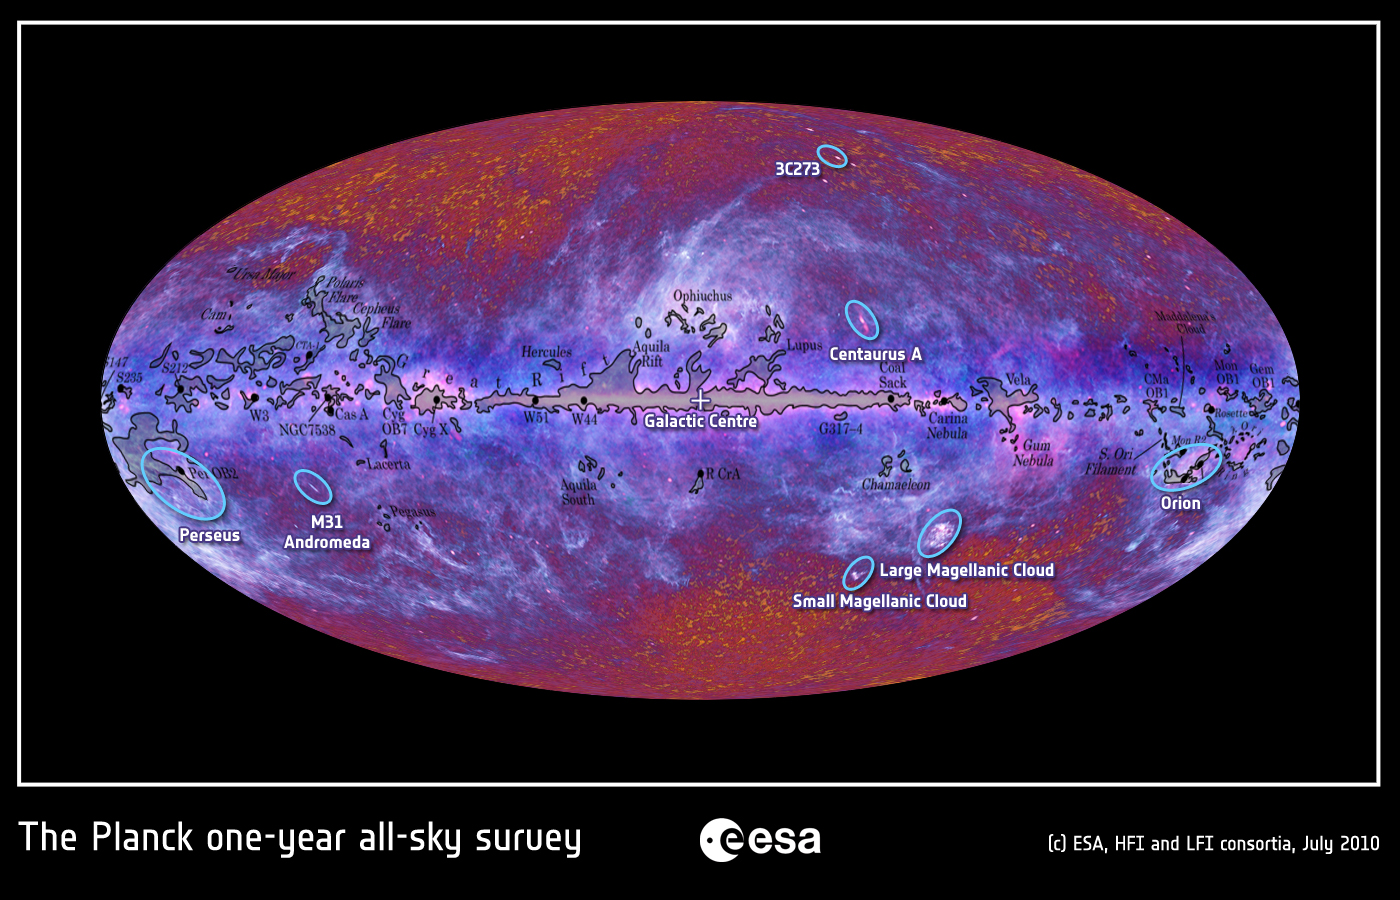
\includegraphics[width=\textwidth,height=!]{./A/PLANCK_FSM_03_Black_Regions_v02_B,0.jpg}
\end{center}
}

\frame{\frametitle{Example star forming region: Aquila Rift - Planck} 
\begin{center}
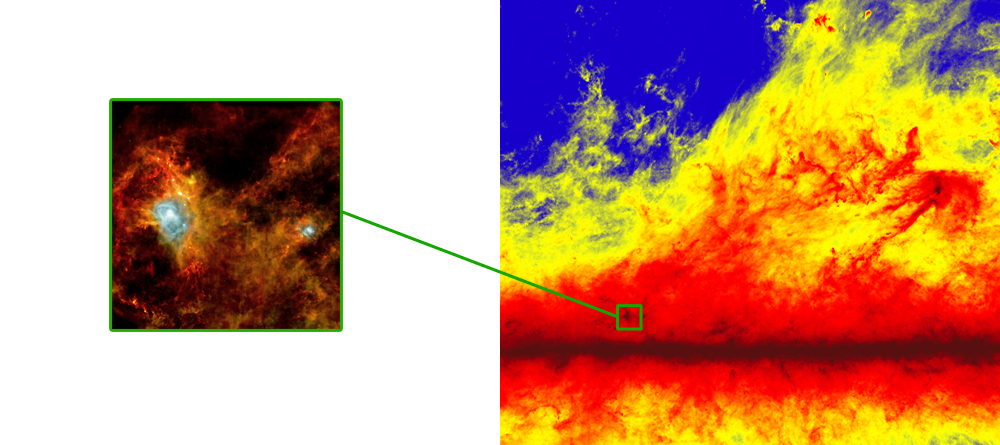
\includegraphics[width=\textwidth,height=!]{./A/P857_with_Aquila_white,2.jpg}
\end{center}
Left: Herschel, Right: Planck 
}




%
\addtocounter{part}{1}

\part[II]{Microscopic Processes}
\begin{frame}
  \partpage
  \tableofcontents[part=2]
\end{frame}



%\begin{frame}\frametitle{Microscopic processes in the ISM}
%
%%\begin{minipage}[t]{13cm}
%%\end{minipage}
%
%\vspace{-1cm}
%\begin{enumerate}
% \item Thermal equilibrium \label{item:Teq}
% \begin{enumerate} 
%  \item  Cooling of the  ISM - collisional excitation \label{item:Teq_cool}
%  \begin{enumerate} 
%    \item ionic excitation \label{item:Teq_cool_ion}
%%    \begin{enumerate} 
%%      \item cooling of H\,{\sc ii} regions \label{item:Teq_cool_hii}
%%      \item cooling of the neutral ISM \label{item:Teq_cool_neutral}
%%    \end{enumerate}
%    \item molecular excitation - CO \& H$_2$ \label{item:Teq_cool_molecule}
%    \item summary: diatomic molecules \label{item:Teq_cool_molstruct}
%   \end{enumerate}
%  \item Cooling of the  ISM - radiative transitions \label{item:Teq_cool_rad}
%  \begin{enumerate}
%    \item  Interaction with electromagnetic radiation \label{item:Teq_cool_rad_H}
%    \item  Transition probabilities \label{item:Teq_cool_rad_prob}
%\end{enumerate}
%\item heating of the  ISM \label{item:Teq_heat}
%%\begin{enumerate}
%%\end{enumerate}
%\end{enumerate}
%\item Molecule formation \label{item:molec}
%\begin{enumerate} 
%\item \label{item:molec_grain} grain catalysis of the formation process of  H$_2$
%\item \label{item:molec_H3+}Molecule formation - the
%role of H$_3^+$.
%\item \label{item:molec_valid} Validation of the ion-molecule model.
%\end{enumerate}
%\item \label{item:fractio} Chemical Fractionation
%\end{enumerate}
%
%
%
%\end{frame}

\section{Thermal Equilibrium of the ISM}

 \begin{frame}\frametitle{Thermal Equilibrium of the ISM}



\centering

\[  \underbrace{n \frac{d}{dt} \left( \frac{3}{2} k T
  \right)}_{\mathrm{variation ~of ~ internal ~E.}} -
\underbrace{kT\frac{dn}{dt}}_{\mathrm{power}}
 = \overbrace{
\stackrel{\mathrm{cooling ~rate}}{\Gamma}  -
\stackrel{\mathrm{heating}}{\Lambda}}^{\mathrm{J~s^{-1}~cm^{-3}}}\]

\raggedright
In steady state, $dn/dt = dT/dt = 0$, so the temperature $T$
is determined by  $\Lambda(T)  = \Gamma(T) $.


\end{frame}

\subsection{Cooling of the ISM: detailed balance, critical density}


\begin{frame}\frametitle{Cooling of the ISM}


Radiative cooling (ref.  Dyson \& Williams, Chap. 3, Spitzer, Chap. 4 \&
6, Osterbrock, Chap. 3). \medskip


\centering
\begin{minipage}[t]{6cm}
\begin{eqnarray*}
 A + B  & \rightarrow &  A + B^{\star} \\
 B^{\star} & \rightarrow  & B + h\nu  
\end{eqnarray*}
\end{minipage} 
\hfill
\begin{minipage}[t]{19cm}
Requisites for a mechanism of radiative cooling
\begin{itemize}

\item frequent encounters, i.e. $A$ \& $B$ abundant
\item $E(B^{\star}) - E(B) \ls k T$. 
\item large rate of $B$ excitations:  high  `collision strength'
\item time scale for radiative decay of  $B^\star$ less than  $\tau_\mathrm{col}$ 
\item large escape probability of the output $h\nu$.
\end{itemize}
\end{minipage} 
\vfill


%\subsubsection{Detailed balance}

\end{frame} \begin{frame}\frametitle{Detailed balance: abundance of
    excited species}

\raggedright

In steady state, the density $n_j$ of species $B^\star$ in level $j$
is determined by an equation of detailed balance, which models systems
with a finite number of microscopic states:
\begin{eqnarray*}
\lefteqn{\sum_k    \left(    \left\{ \begin{array}{c}  n_\mathrm{e} \\
    n_\mathrm{H_2} \\  n_\mathrm{H_I} \end{array} \right\}    n_j
  \gamma_{jk} +  {n}_{j} B_{jk} J_\nu \right) + \sum_{k<j} \left( A_{jk} n_j  \right)   } \\   
& &     =    \sum_k \left(  n_k      \left\{ \begin{array}{c}  n_\mathrm{e} \\  n_\mathrm{H_2} \\  n_\mathrm{H_I} \end{array} \right\}  \gamma_{kj} + B_{kj} J_\nu n_k \right) + \sum_{k>j} \left( n_k A_{kj} \right),
\end{eqnarray*}
which we may also write using a  simplified notation: 
\[\sum_{i{\neq}j}
{n}_{j}{C}_{ji} + {n}_{j}{B}_{ji} U_{\nu_{ji}} +
\sum_{i<j}{n}_{j}{A}_{ji} = \sum_{i{\neq}j}{n}_{i}{C}_{ij} +  {n}_{i}{B}_{ji} U_{\nu_{ij}} + \sum_{i>j}{n}_{i}{A}_{ij}. 
\]

\vfill



%\end{frame} \begin{frame}\frametitle{\textcolor{red}{B$_1$} Enfr\'{\i}amento   del ISM  }
\end{frame} \begin{frame}\frametitle{Detailed balance: rate of collisonal excitation}

For any collision partner (i.e. either $\begin{array}{c}  n_\mathrm{e}
\\  n_\mathrm{H_2} \\  n_\mathrm{H_I} \end{array} $ ), the specific rate of
collisional excitations is

\[
\gamma_{jk} = \langle u \sigma_{jk}(u) \rangle = \frac{4}{\sqrt{\pi}} \left(\frac{m_r}{2kT} \right)^{3/2} \int_0^\infty du ~ u^3 \sigma_{jk}(u) \exp\left(  - \frac{m_r}{2kT} u^2 \right).
\]

 the specific rate (i.e. per pair of  particles, in units of
m$^{3}$~s$^{-1}$) of collisional de-excitations $\gamma_{kj}$ must be
related to $\gamma_{jk}$: in thermodynamic equilibrium any microscopic
process must be balanced by its inverse ({\em principle of detailed
balance}, otherwise the distribution functions would depend on $t$ and
there would be no equilibrium).

%\end{frame} \begin{frame}\frametitle{\textcolor{red}{B$_1$} Enfr\'{\i}amento   del ISM  }

\end{frame} \begin{frame}\frametitle{Milne relations}

In {\bf LTE} the rate of collisional excitations $j\rightarrow k$ with
relative velocity $\vec{u} \in [\vec{u},\vec{u}+d\vec{u}]$ must equal
the rate of de-excitations $k \rightarrow j$ in the corresponding
velocity range $\vec{v}$, \[
n^\mathrm{LTE}_j \begin{array}{c}  n_\mathrm{e} \\  n_\mathrm{H_2} \\  n_\mathrm{H_I} \end{array}  \sigma_{jk}(u) f(u)  u d\vec{u}  = 
n^\mathrm{LTE}_k \begin{array}{c}  n_\mathrm{e} \\  n_\mathrm{H_2} \\
n_\mathrm{H_I} \end{array}  \sigma_{kj}(v) f(v)  v d\vec{v}  , \]
with   $ f(u) =   \left(\frac{1}{\pi}\frac{m}{2kT} \right)^{3/2}
\exp\left(-\frac{m}{2kT} u^2 \right) $,  and~~ $ \frac{1}{2}m_r v^2 =
\frac{1}{2} m_r u^2 - E_{jk}$~\footnote{note threshold excitation energy},  
%\centering
\[\stackrel{\textcolor{red}{\mathrm{tarea}}} \Longrightarrow  ~~~~~  g_j u^2 \sigma_{jk}(u) = g_k v^2 \sigma_{kj}(v),~\text{or} \]
\[ C_{kj}=C_{jk} \frac{g_{j}}{g_{k}} e^{E_{jk}/kT} .\] 


%\subsubsection{Critical density}

\end{frame} \begin{frame}\frametitle{Critical density}

The {\em critical density} is defined as the density at which the rate
of collisonal de-excitations is equal to the rate of radiative
de-excitations:

\[\sum_{k<j} C_{kj} = \sum_{k<j} A_{jk} .\]

A good cooling mechanism is therefore one that involves abundant
species, an effective collision strength $\gs$1, a critical density
$n_\mathrm{crit} \gg n_\mathrm{e}$, and opticallly thin transport of
the output $h \nu_{jk}$.



\end{frame}
\subsection{Ionic \& atomic  cooling of the ISM}
 \begin{frame}\frametitle{Ionic  \& atomic  cooling of the ISM}

For ionic collisions, the cross-section of collisional excitation
highlights the Coulomb cross-section.
\[ \sigma_{jk}(E)=\frac{\pi a_{\circ}^{2}  \Omega_{jk}(E)}{E/E_{\circ}}, \]
where $E_{\circ}$ is ~1~Rydberg, $a_{\circ}$ is the Bohr radius, and
$\Omega_{jk}(E)$ (of order 1), is the {\em collision strength} as a
function of  kinetic energy $E$. Finally the rate of excitations $j
\rightarrow k$ (with units of s$^{-1}$) is (\textcolor{red}{tarea}),
\[
C_{jk}= \left\{ \begin{array}{c} n_\mathrm{e} \\ n_\mathrm{H_2} \\
n_\mathrm{H_I} \end{array} \right\} {\sqrt{\frac{2\pi}{kT}}}
{\left(\frac{h}{2\pi}\right)}^{2}
\frac{1}{m_r^{3/2}} \frac{\Gamma_{jk}}{g_{j}} e^{-E_{jk}/kT},
\] where  $\Gamma_{jk}$,  the   {\em  effective collision strength},
is the Maxwellian average of $\Omega(E)$.

%\end{frame} \begin{frame}\frametitle{\textcolor{red}{B$_1$} Enfr\'{\i}amento   del ISM  }

\end{frame} \begin{frame}\frametitle{Fine structure cooling in the IR}

In LS coupling energy levels are ordered according to the Hund rules
(Shu I Chap. 27):

\begin{itemize}
\item Higher S $\rightarrow$ lower energy
\item Higher L $\rightarrow$ lower energy
\item Higher J $\rightarrow$ higher energy if less than half-filled,
lower energy if more than half-filled
\end{itemize}

Spectroscopic notation in spin-orbit coupling (ver Shu
I,27):
\LARGE \\ \medskip
\( \mathrm{^{2S+1} L_J   } \) \normalsize, with degeneracy (2~J+1)

\textcolor{blue}{\bf Examples:} 
\begin{itemize}
\item  $[$Ar\,{\sc vi}$]$~4.52$\mu$m, $^2$P$_\frac{1}{2}\leftarrow ^2$P$_\frac{3}{2}$, Z=18
\item  $[$Al\,{\sc vi}$]$~3.65$\mu$m, $^3$P$_2\leftarrow ^3$P$_1$, Z=13
\end{itemize}


\end{frame} \begin{frame}\frametitle{Ar\,{\sc vi}  $^2$P$_\frac{3}{2}$
  population}

\begin{center}
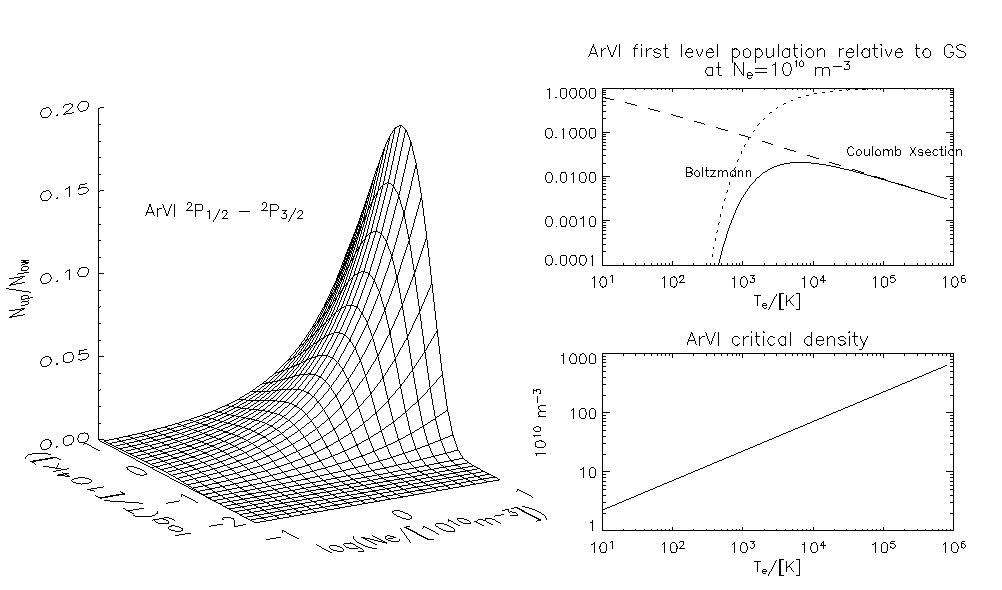
\includegraphics[width=\textwidth,height=!]{./B/ArVI_pop.pdf}
\end{center}

\end{frame} \begin{frame}\frametitle{ Ar\,{\sc vi}  $^2$P$_\frac{3}{2}$
  population}


\begin{center}
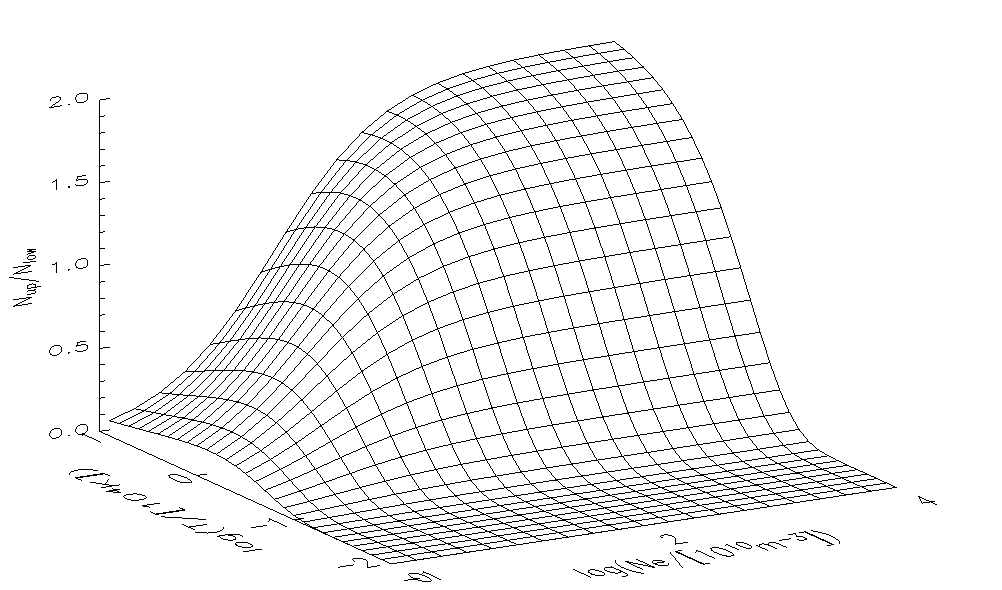
\includegraphics[width=\textwidth,height=!]{./B/ArVI_pop_xtd.pdf}
\end{center}

%%%%%%%%%%%%%%%%%%%%%%%%%%%%%%%%%%%%%%%%%%%%%%%%%%%%%%%%%%%%%%%%%%%%%%%%%%%
%%%%%%%%%%%%%%%%%%%%%%%%%%%%%%%%%%%%%%%%%%%%%%%%%%%%%%%%%%%%%%%%%%%%%%%%%%%
%%%%%%%%%%%%%%%%%%%%%%%%%%%%%%%%%%%%%%%%%%%%%%%%%%%%%%%%%%%%%%%%%%%%%%%%%%%

\end{frame} \begin{frame}\frametitle{Cooling of H\,{\sc ii} regions}
%\leftheader{B-\ref{item:Teq_cool_hii}:  Cooling of }

%\end{frame} \begin{frame}\frametitle{\textcolor{red}{B$_1$} Enfr\'{\i}amento  de regiones H\,{\sc ii} }

For gas in a steady state, where every ionization event is balanced by
a recombination event (case of a nebula photoionised by OB stars), the
cooling mechanisms are:


\begin{enumerate}

\item Recombination radiation (postponed to chapter on photoionised nebulae)
\item Continuum emission (free-free, bound-free):  $A + B   \rightarrow   A +
  B + h\nu $ (postponed to chapter on
  photoionised nebulae)

\item Collisionally excited line emission: 
$$\Lambda_{CE}= \sum_X \sum_i n(X,i) \sum_{j < i} A_{i,j}\, (E_i -
E_j)$$ e.g.
\begin{itemize}
\item   $[$O\,{\sc ii}$]\lambda\lambda$3726,3729 ~ $\mathrm{^4S_{3/2} \leftarrow ^2\!D_{3/2,5/2} } $.
%\item   $[$S\,{\sc iii}$]\lambda\lambda$9071,9533 ~ $\mathrm{^3P_{2,1} \leftarrow ^1D_{2} } $.
\item   $[$O\,{\sc iii}$]\lambda\lambda$4959,5007 ~ $\mathrm{^3P_{2,1} \leftarrow ^1D_{2} } $.
\end{itemize}

\end{enumerate}


\end{frame} \begin{frame}\frametitle{Cooling of H\,{\sc ii} regions: collisionally excited line radiation}

\begin{center}
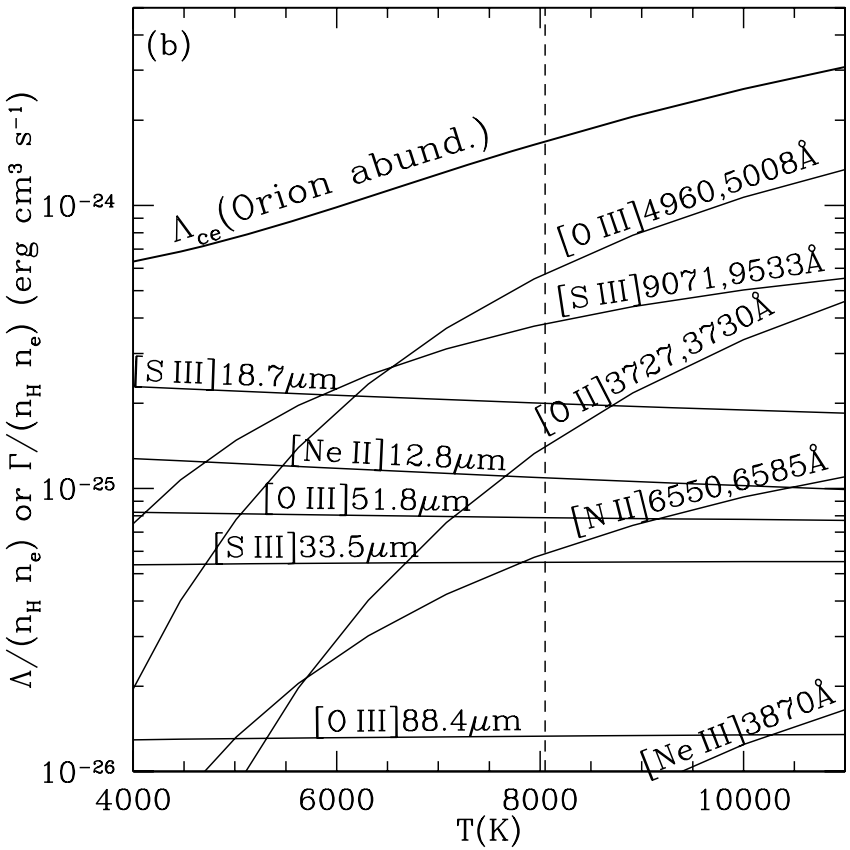
\includegraphics[width=0.8\textwidth,height=!]{./B/cooling_CE.png}
\end{center}

\end{frame} \begin{frame}\frametitle{Cooling of H\,{\sc ii} regions: collisionally excited line radiation}
$z \sim z_{\odot}$
\begin{center}
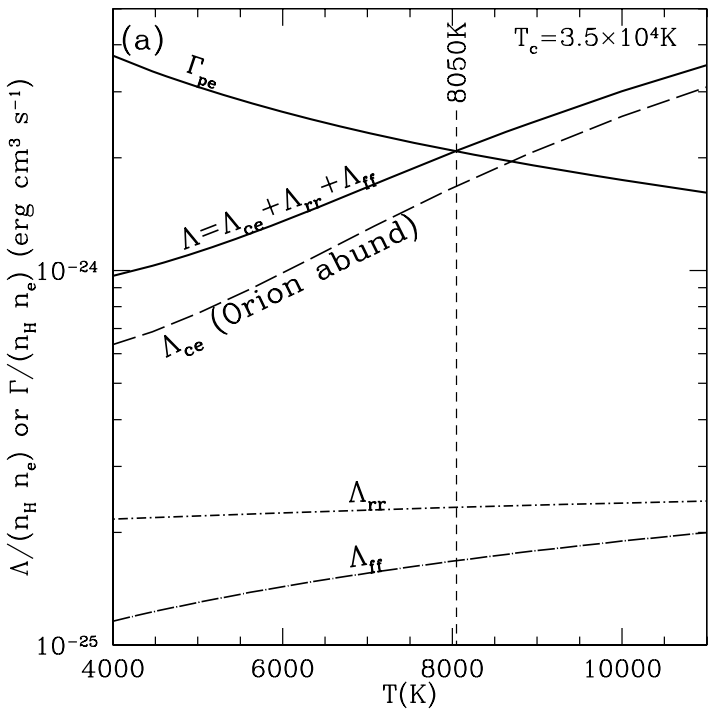
\includegraphics[width=0.8\textwidth,height=!]{./B/heating_cooling.png}
\end{center}


\end{frame} \begin{frame}\frametitle{Cooling of H\,{\sc ii} regions: collisionally excited line radiation}
$z \sim 0.1 z_{\odot}$
\begin{center}
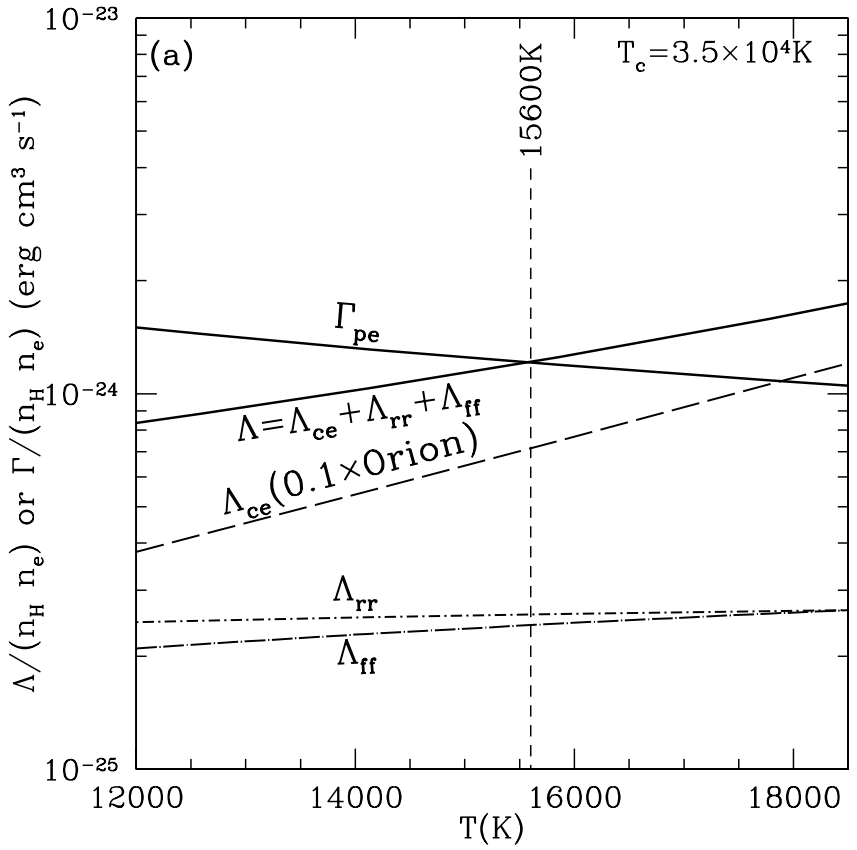
\includegraphics[width=0.8\textwidth,height=!]{./B/cooling_01.png}
\end{center}



\end{frame} \begin{frame}\frametitle{Cooling of H\,{\sc ii} regions: collisionally excited line radiation}
$z \sim 3 z_{\odot}$
\begin{center}
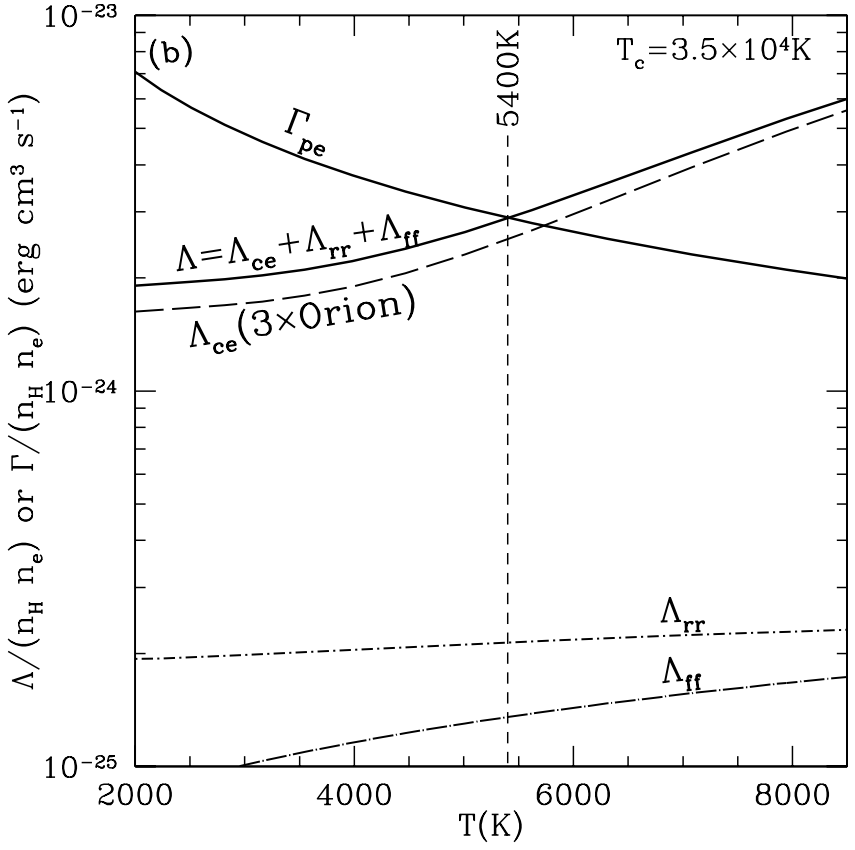
\includegraphics[width=0.8\textwidth,height=!]{./B/cooling_3x.png}
\end{center}






\end{frame} \begin{frame}\frametitle{Cooling of the neutral ISM}
%\end{frame} \begin{frame}\frametitle{\textcolor{red}{B$_1$} Enfr\'{\i}amento  del ISM neutro - \'atomos e {\em iones} }

%1576800.         [C II]      M1        2Po-2Po         1/2-3/2           .00 -       63.42
% 631850.         [O I]       M1         3P-3P            2-1             .00 -      158.26
%1455350.         [O I]       M1         3P-3P            1-0          158.26 -      226.98
% 348152.         [Si II]     M1        2Po-2Po         1/2-3/2           .00 -      287.23

Occurs through excitation of low-lying electronic states, fine
structure levels dominate.

Examples: Table~3.1 in Dyson \& Williams complemented by the list of
lines in {\tt http://www.pa.uky.edu/$\sim$peter/atomic/}

\begin{center}
\begin{tabular} {lll}
Transition   &    collision partner &  $\Delta E / k$ \\   \hline 
$[$C\,{\sc i}$]$~$\lambda$157.7\,$\mu$m ~ $\mathrm{^2P_{1/2} \leftarrow ^2P_{3/2} } $    & H,e,H$_2$  &   92~K \\
$[$Si\,{\sc ii}$]$~$\lambda$34.8\,$\mu$m ~ $\mathrm{^2P_{1/2} \leftarrow ^2P_{3/2} } $    & e  &   92~K \\
$[$O\,{\sc i}$]$~$\lambda$63.2\,$\mu$m ~ $\mathrm{^3P_{1} \leftarrow ^3P_{2} } $    & H,e  &   228~K \\
$[$O\,{\sc i}$]$~$\lambda$145.5\,$\mu$m ~ $\mathrm{^3P_{0} \leftarrow ^3P_{2} } $    & H,e  &   326~K \\
\end{tabular}
\end{center}




\end{frame} 

%

\begin{frame}\frametitle{Molecular excitation - CO \& H$_2$}

%\end{frame} \begin{frame}\frametitle{\textcolor{red}{B$_1$} Enfr\'{\i}amento  del ISM neutro - H$_2$ }

%1576800.         [C II]      M1        2Po-2Po         1/2-3/2           .00 -       63.42
% 631850.         [O I]       M1         3P-3P            2-1             .00 -      158.26
%1455350.         [O I]       M1         3P-3P            1-0          158.26 -      226.98
% 348152.         [Si II]     M1        2Po-2Po         1/2-3/2           .00 -      287.23

%Van Dishoeck, 2004, ARA\&A, 42, 119

{\em ISO} observations (Van Dishoeck, 2004, ARA\&A, 42, 119)
suggest that the contribution from H$_2$ cooling is more important
than estimates based on {\em IRAS} data: H$_2$ is among the brightest
emission lines in molecular clouds exposed to UV radiation, as for
instance in Orion~KL (note prominent dust continuuum):


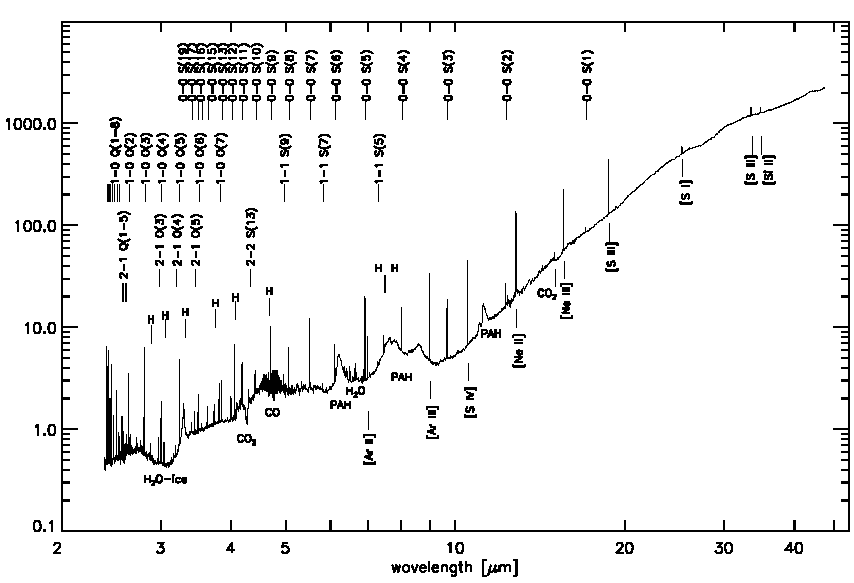
\includegraphics[width=0.8\textwidth,height=!]{./B/dishoeck_fig3.pdf}

\end{frame} \begin{frame}\frametitle{fluorescent H$_2$: not a gas coolant}

The rotational excitation of the ground vibrational state of H$_2$ is
usually collisional (i.e. thermal), while higher vibrational states are excited by fluorescence (hence not a cooling process). 

\medskip

$\Rightarrow$ near-IR rovib H$_2$ is usually fluorescent, so not a
coolant (except some of the lower-level rovib lines, in shocked regions). 

\vfill

\end{frame} \begin{frame}\frametitle{Dust continuum: not a gas coolant}

The most luminous spectral component in the molecular ISM is the
mid-IR to far-IR continuum, due to dust. Dust is responsible for
transporting the UV radiation of the exciting stars, but is not always
coupled to the molecular gas. Collisions are efficient dust heating
sources in the denser media only, such as dense SNRs or dense
circumstellar disks.

%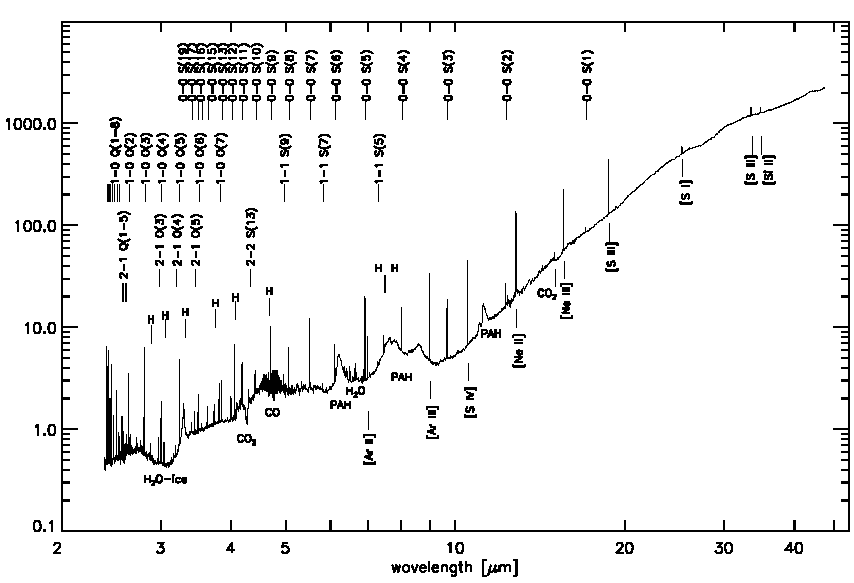
\includegraphics[width=0.7\textwidth,height=!]{./B/dishoeck_fig3.pdf}
\centering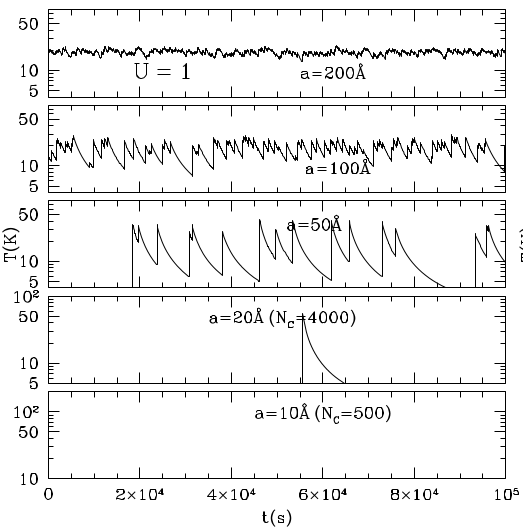
\includegraphics[width=0.6\textwidth,height=!]{./B/grain_temp.png}

\end{frame} \begin{frame}\frametitle{CO rotational-line cooling}
%\begin{minipage}{12.5cm}
%The main cooling agents for cold molecular clouds are low-level
%rotational transitions of CO in the sub-mm. (Figure 2.11 from Tielens
%2005).
%\end{minipage}
%\hfill
%\begin{minipage}{13cm}
%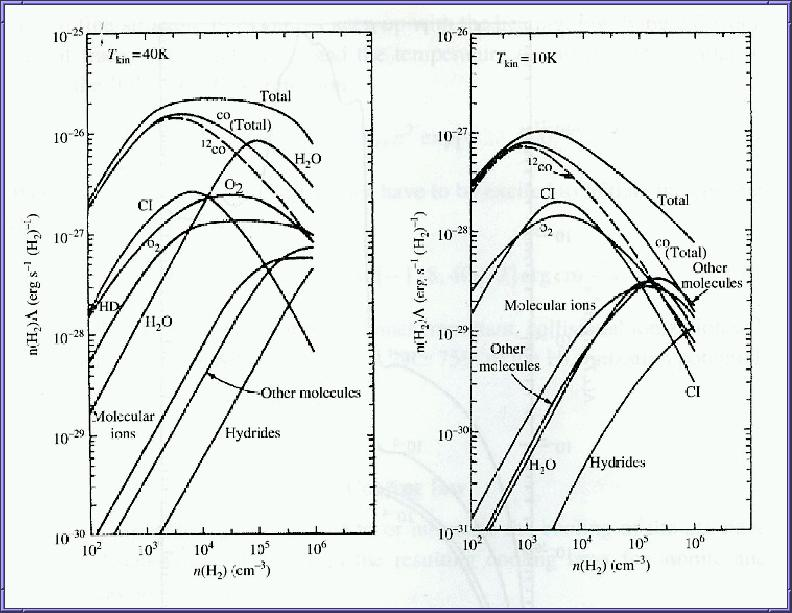
\includegraphics[width=13cm,height=!]{./B/CO_cooling_Tielens.jpg}
%\end{minipage}

The main cooling agents for cold molecular clouds are low-level
rotational transitions of CO in the sub-mm. (Figure 2.11 from Tielens
2005).
\begin{center}
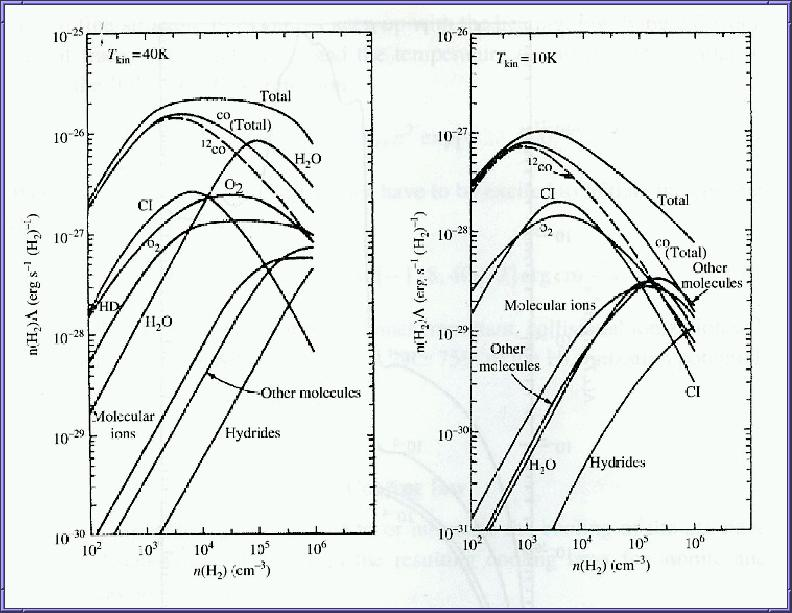
\includegraphics[width=0.8\textwidth,height=!]{./B/CO_cooling_Tielens.jpg}
\end{center}




\end{frame} 


%\subsubsection{Molecular structure}
\subsection{Molecular excitation \& molecular structure}
\begin{frame}\frametitle{Summary: diatomic molecules}

In the Born-Oppenheimer approximation the Hamiltonian for a diatomic
molecule AB separates, $H = H_\mathrm{AB} + H_\mathrm{el} $, where
$H_\mathrm{AB}$ represents the kinetic energy of the nuclei, and
$H_\mathrm{el}$ all the rest. It is also customary to factorize $\phi =
\phi_\mathrm{el}
\phi_\mathrm{AB}$ and obtain  \footnote{provided additional
approximations according to Messiah, Vol. 2, XVIII.64 (p791), but
exactly according to Shu I, 28. Probably valid only for processes
slower than a rotation period.}:
\[H_\mathrm{el}  \phi_\mathrm{el} = E_\mathrm{el}(R)~  \phi_\mathrm{el}, \] 
\[H_\mathrm{AB}  \phi_\mathrm{AB} +  E_\mathrm{el}(R)~ \phi_\mathrm{AB} = E~ \phi_\mathrm{AB}, \] 
and using the centre of mass coordinates, $\phi_\mathrm{AB} =
\phi_\mathrm{trans}(\vec{X}_\mathrm{CM}) \phi_\mathrm{intern}(\vec{R})
$,
\[ -\frac{\hbar^2}{2M} \nabla^2_\mathrm{CM} \phi_\mathrm{trans}  = E_\mathrm{trans} ~\phi_\mathrm{trans} \]
\[ -\frac{\hbar^2}{2\mu} \nabla^2_{\vec{R}} \phi_\mathrm{intern} + E_\mathrm{el}(R) ~\phi_\mathrm{intern}  = E_\mathrm{intern} ~\phi_\mathrm{intern},\]
with $E=E_\mathrm{intern}+E_\mathrm{trans}$.
\end{frame} \begin{frame}\frametitle{}
The Laplacian in spherical coordinates,
\[ \nabla^2_{\vec{R}} = \frac{1}{R^2} \left[ \frac{\partial}{\partial R} \left( R^2  \frac{\partial}{\partial R}  \right) - \frac{L^2}{\hbar^2} \right], \]
inspires the decomposition of the wave function for the internal
degrees of freedom in spherical armonics,
\[\phi_\mathrm{intern}(\vec{R}) = \frac{1}{R} Z_\mathrm{vib}(R) Y_{Jm}(\theta,\varphi), \]
The 1-D equation for $Z_\mathrm{vib}(R)$ is a function of
$E_\mathrm{el}(R)$, the energy eigenvalue of the electronic wave function:
\[-\frac{\hbar^2}{2\mu} \frac{d^2\,Z_\mathrm{vib}}{dR^2} +
E_\mathrm{el}(R)  Z_\mathrm{vib} = \left[ E_\mathrm{intern}  - \frac{
    J (J + 1) \hbar^2} {2\mu\,R^2} \right] Z_\mathrm{vib}. \]


\end{frame} \begin{frame}\frametitle{} 
In the armonic approximation we expand the 1-D equation for
$Z_\mathrm{vib}$ about $R_{\circ}$, the AB separation in the
fundamental state, highlighting the natural frequency $\mu
\omega_\circ \equiv E^{\prime\prime}_{el}(R_\circ)$ :
\[ - \frac{\hbar^2}{2\mu} \frac{d^2 Z_\mathrm{vib}}{dx^2} + \frac{\mu}{2} \omega^2_\circ x^2 Z_\mathrm{vib} = E_\mathrm{vib} Z_\mathrm{vib}, \]
\[ x \equiv R - R_{\circ} , ~~~\mathrm{and}\] 
\[ \boxed{ E_\mathrm{intern} = E_\mathrm{el}(R_\circ) + E_\mathrm{vib} + E_\mathrm{rot},} \] 
\[ E_\mathrm{rot} = J (J+1) \, \frac{\hbar}{2\mu R^2_\circ} \equiv J
(J+1) B, ~~~~\textcolor{blue}{B: \mathrm{ ~rotational~constant}}, \]
\[ E_\mathrm{vib}  = (v + \frac{1}{2} ) \hbar \omega_\circ.  \]


\end{frame} \begin{frame}\frametitle{} 

The quantum numbers that determine the nuclear state of the molecule
are $J,m,v$. Note the rigid body assumption: $\phi_\mathrm{el}$ is
independent of $J$, which is the fundamental hypothesis implicit in
the decomposition $\phi = \phi_\mathrm{el} \phi_\mathrm{AB}$. The
quantum numbers that characterise the electronic state of the molecule
are $\Lambda$, and $S$, where $\Lambda$ corresponds to the projection
of $L_\mathrm{tot}$ along the internuclear axis\footnote{the only
component of $\vec{L}$ that is conserved in diatomic molecules}, and
$S$ is the total spin.




\end{frame}

\subsection{Atomic/molecular coupling with radiation}

 \begin{frame}\frametitle{ Interaction with electromagnetic radiation}




The coupling term between charged particles and the electromagnetic
field,
$\vec{p_i}\cdot\vec{A}(\vec{k}\cdot\vec{x}-wt)$\footnote{when
substituting 
$\vec{p} \rightarrow \vec{p}-\frac{q}{c}\vec{A}$, and neglecting terms
in  $A^2$ (OK for the ISM) see Shu I, 21}, can be expressed 
through an expansion in $\vec{k}\cdot\vec{x}$ as $H_\mathrm{int}
= H_\mathrm{d} + H_\mathrm{M} + H_\mathrm{Q}$ (see Shu I,24), for which
\[ H_\mathrm{d} = - \vec{E}\cdot\vec{d} ~ (\mathrm{zeroth~order})\]
where, for a molecule,  $\vec{d} = \vec{d}_\mathrm{el} + \vec{d}_\mathrm{nuc}$.
\[ H_\mathrm{M} = - \vec{B}\cdot\vec{M} ~  (\mathrm{first~order}) \]
where the magnetic dipole moment $\vec{M} \propto \vec{L} $, and
\[ H_\mathrm{Q} = - \frac{e}{6}\vec{\nabla}\vec{E}:(3 \vec{x}\vec{x} -
|\vec{x}|^2 {\Bbb I})  ~~  (\mathrm{also ~order~one}).  \]
In general  $H_\mathrm{M} >  H_\mathrm{Q}$. 



\end{frame} \begin{frame}\frametitle{Bound-bound
transition probabilities and cross-sections}

In time-dependent perturbation theory, the rate of radiative
excitations $i \rightarrow f$ is:
%\[ \frac{dP_{if}}{dt} = \frac{4 \pi e \omega^2_{if}}{3 h c^2} {\frak N}(\omega_{if})    \left| \langle \phi_f| H_\mathrm{int} |\phi_i \rangle \right|^2. \] 
%\[ \frac{dP_{if}}{dt} \propto   \frac{4 \pi e \omega^2_{if}}{3 h c^2} {\frak N}(\omega_{if})    \left| \langle \phi_f| H_\mathrm{int}(\omega) |\phi_i \rangle \right|^2. \] 
\[ \frac{dP_{if}}{dt} \propto    {\frak N}(\omega_{if})    \left| \langle \phi_f| H_\mathrm{int}(\omega) |\phi_i \rangle \right|^2. \] 
In a cubic box where the ocupation number of state 
$\vec{n}$ is ${\frak N}$, the density of states is $d^3\vec{n} = V
d^3\omega / (2\pi c )^3$, with a volume $V \rightarrow \infty $.

The absorption cross-section $\textcolor{red}{\sigma_{if}}$ derives
from $ P_{if} = N_f/N_i \propto $ \# of absorbed photons
\footnote{note   {\em optically thin} case: $dN_f = -\Gamma N_f dt + \frac{d P_{if}} {dt} N_i dt $.}: 
\[ P_{if} = \int d^3\vec{n} \, \frac {{\frak N}(\vec{n})} {V}   c~ t~  \textcolor{red}{\sigma_{if}}  ~ \Rightarrow  ~  \frac{dP_{if}}{dt} = \int_0^\infty \textcolor{red}{\sigma_{if}}~ c~ {\frak N}(\omega) ~\frac{4 \pi \omega^2}{(2\pi)^3 c^2} d\omega\]
Identifying (see Shu I, 22, 23), we obtain
% \[ \sigma_{if} = \frac{4 \pi^2}{3} \left( \frac{e^2}{m_e } \right)    \left|  \langle \phi_f| H_\mathrm{int} |\phi_i \rangle \right|^2   \delta(\omega-\omega_{if}).  \]
\[ \sigma_{if} \propto    \left|  \langle \phi_f| H_\mathrm{int}(w) |\phi_i \rangle \right|^2   \delta(\omega-\omega_{if}).  \]


\end{frame} \begin{frame}\frametitle{Oscilator strength}

For the electric dipole Hamiltonian, one gets
 \[ \sigma_{if} = \frac{4 \pi^2}{3  \hbar c }     \left|  \langle \phi_f| \vec{d} |\phi_i \rangle \right|^2   \delta(\omega-\omega_{if}),  \]
which is usually expressed in terms of the oscilator strength $f_{if}$,
 \[ \sigma_{if} = \frac{\pi e^2}{m_e c }  f_{if}     \delta(\nu-\nu_{if}),  ~~\text{con} ~~~
f_{if} \equiv \frac{ 4 \pi m_e } {3 e^2 \hbar} \nu_{if} \left| \langle
\phi_f| \vec{d} |\phi_i \rangle \right|^2. \] For a single electron
 with position $\vec{x}$, \[ f_{if} = \frac{ 2 m_e ( \omega_{if}
\langle f | \vec{x}| i \rangle )^2}{3 \hbar w_{if}}, \] which is
roughly the ratio between the vibrational potential energy of the
electron and that of the radiated photon.



\end{frame} \begin{frame}\frametitle{Relationship with Einstein coeficients}

The equation of detailed balance, 
\[n_i B_{if} J_{\nu_{if}} = n_f A_{fi} + n_f B_{fi} J_{\nu_{fi}}, \]
and the LTE relationships,
\[\frac{n_f}{n_i} = \frac{g_f}{g_i} \exp(-\frac{h\nu_{if}}{kT}),
~~~\text{and}~~~J_{\nu} = B_{\nu}(T),~~\text{lead~to} \]
\[ A_{fi} = \frac{g_i}{g_f} (2 h \nu^3 / c^2 ) B_{if} , ~~~~~~~~ B_{fi} = \frac{c^2}{2 h \nu^3} A_{fi} = (g_i / g_f ) B_{if}, \]
where the rate of stimulated  excitations is related to the
oscilator strength\footnote{using the requirement $n_i B_{if} J_{\nu_{if}} = \int d\nu \int d\Omega
\sigma_{if} n_i \frac{J_\nu}{h\nu} = \int d\nu  4\pi \sigma_{if} n_i \frac{J_\nu}{h\nu}$}
:
\[ B_{if} = \frac{4 \pi^2 }{h \nu} \frac{e^2}{m_e c} f_{if}.\]



\end{frame} \begin{frame}\frametitle{Selection rules}

\begin{itemize} 
\item Electric dipole
\begin{itemize} 
\item  atoms: $\Delta l = 1$, $\Delta m = 0$. 
\item  molecules: 
\begin{itemize}  
\item vibrational-rotational transitions, or rovibrational,  $\Delta J
  = \pm 1$, $\Delta m = 0$,$\Delta v = \pm 1$,\\ allowed when $\Lambda \neq
0$, $\Delta J = 0$ \footnote{ {\em Lambda doubling}, two
states $\pm\Lambda$ for each $J$. Example: hyperfine structure of the
OH $\Lambda$ doublet at $\sim$1.7~GHz.}.
\item  electronic transitions, $\Delta \Lambda = 0, \pm 1$, $\Delta S = 0$\\
\item  electronic-vibrational-rotational transitions 
  (i.e. {\em vibronic} transitions): $\Delta J = 0, \pm 1 $, $\Delta m
  = 0, \pm 1$ and $\Delta J \neq 0$ si $\Lambda = \Delta \Lambda = 0$
  and if  $J = 0$.

  \medskip 

$\Delta J  =   \left\{  \begin{array}{l} 
+1~ \rightarrow~  \text{ R branch} \\
0~ \rightarrow~  \text{ Q branch} \\
-1~ \rightarrow~  \text{ P branch}  \end{array} \right. 
$
\end{itemize}
\end{itemize}
\item  magnetic dipole,  atoms: $\Delta l = 0$, $\Delta m = 0, \pm 1$. 
\item  electric quadrupole,  atoms: $\Delta l = 0, \pm 2$,
  $\Delta m = 0, \pm 1, \pm 2$, rotational transitions in molecules
  $\Delta J = 0, \pm 1, \pm 2$.
\end{itemize}



\end{frame} \begin{frame}\frametitle{Selection rules -- CO\footnote{{Subaru - IRCS + echelle
      \& X-disperser, Goto et al. 2003, ApJ, 598, 1038}}}
\vspace{-1cm}

\begin{center}
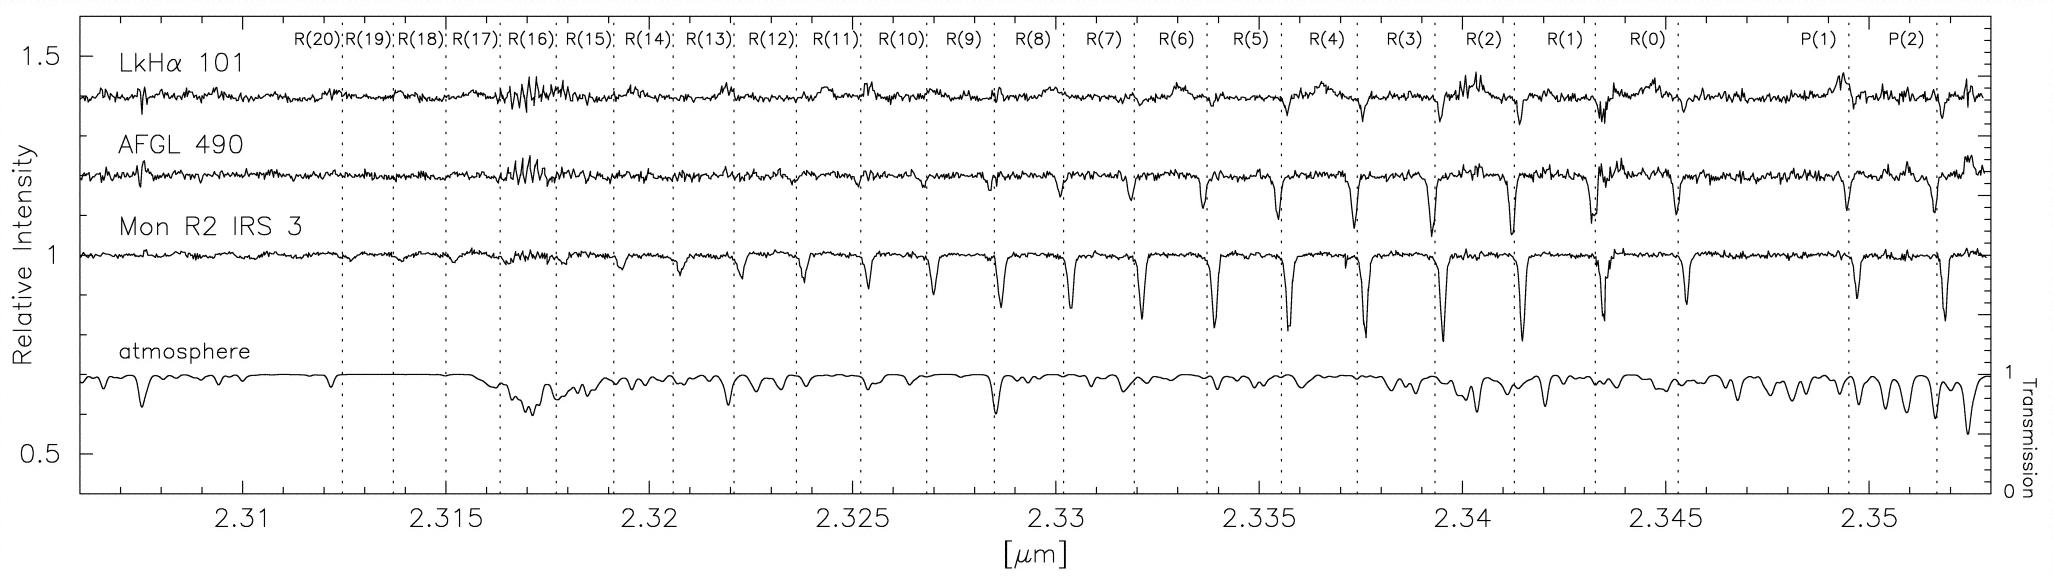
\includegraphics[width=\textwidth,height=!]{./B/CO_subaru_1.jpg}

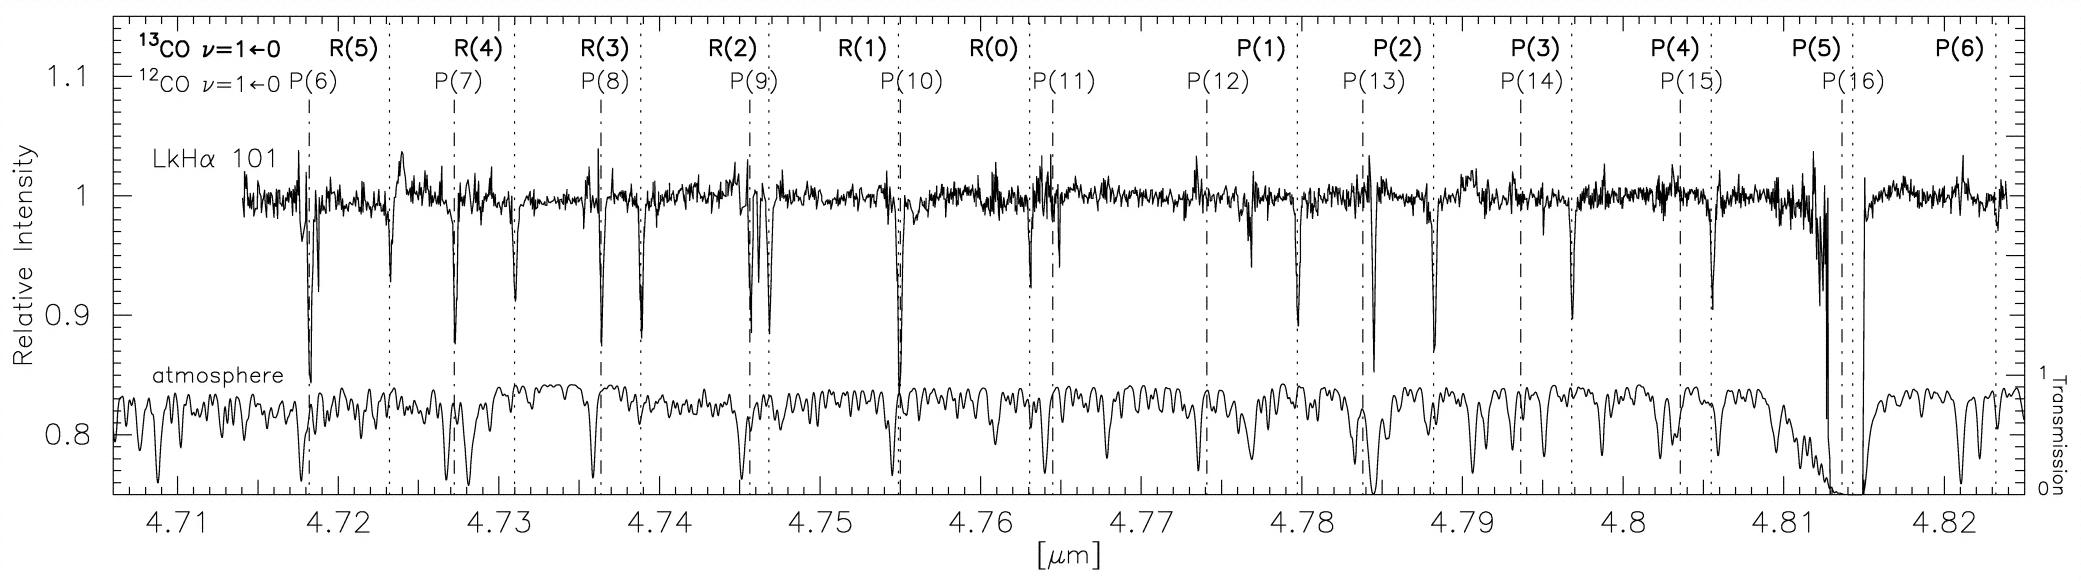
\includegraphics[width=\textwidth,height=!]{./B/CO_subaru_2.jpg}
\end{center}
\vfill



\end{frame} \begin{frame}\frametitle{Selection rules -- H$_2$}

In the case of $H_2$ we have $\vec{d}=0$. Moreover the fundamental
 state is $\vec{L} = 0$, and $\vec{S}=0$, so that $\vec{M}=0$ and all
 low-energy transitions for  $H_2$ are quadrupolar.

Note that the antisymmetry of the nuclear wave function implies that
the state $J=1$ ($J$ odd) is triplet ({\bf Ortho } H$_2$, $I =
S_\mathrm{nuclear} = 1$ ), while $J=0$ ($J$ even) is singlet ({\bf
Para } H$_2$, $I = 0$).\\


In H$_2$ the exclusion principle \footnote{the requirement that the
  wave function be antisymmetric} forbids $\Delta J = 1$, unless the
transition involves a change in spin state. The spin transitions can
only occur through the exchange of protons in collisions. Radiative
transitions between spin states can occur, but at a rate corresponding
to the quadrupolar transitions in the Hamiltonian of the deviations to
the Born-Oppenheimer approximations. \\


\end{frame} \begin{frame}\frametitle{}

In the ISM, {\bf Ortho } and {\bf Para } H$_2$ are effectively
different molecules. The distinction extends to all molecules that
contain H$_2$ radicals.

Rovibrational transitions between an upper level $^1$ and a lower
level $^2$ are written $(v_1-v_2)O(J_2)$, when $J_2-J_1 = -2$,
$(v_1-v_2)Q(J_2)$ when $J_2-J_1 = 0$, $(v_1-v_2)S(J_2)$ when $J_2-J_1
= +2$.



\end{frame} \begin{frame}\frametitle{H$_2$ energy levels}

\begin{minipage}[t]{0.59\textwidth}
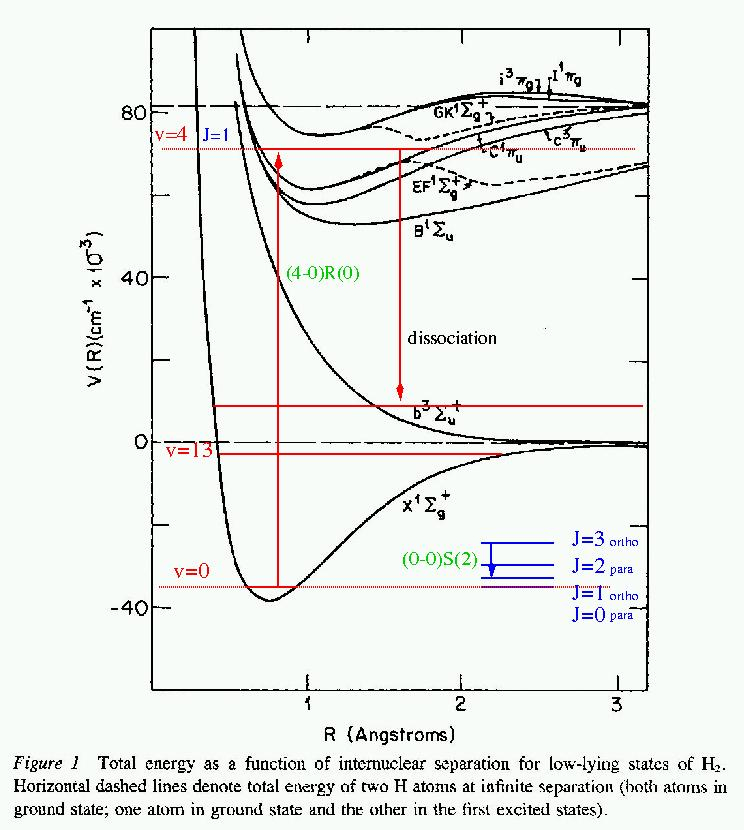
\includegraphics[width=\textwidth,height=!]{./B/h2_levels_xv.jpg}
\end{minipage}
\hfill
\begin{minipage}[t]{0.39\textwidth}
\vspace{-6cm}
$\Lambda = 0, 1, 2, ... $\\ $\Leftrightarrow$ $ \Sigma, \Pi, \Delta$ \\
levels in  $E_\mathrm{el}(R)$:\\ $X,B,C,D$.\\

The energy separation between levels $B$ and $C$ with respect to $X$
are $\sim$ 11~eV and 14~eV.  \\
\end{minipage}
\vfill

%
%\end{frame} \begin{frame}\frametitle{Emisi\'on IR de H$_2$}
%
%\begin{minipage}[t]{13cm}
%Como la tasa de transiciones radiativas en el nivel electr\'onico
%fundamental de H$_2$ es de orden cuadrupolar, la poblaciones de los
%niveles ro-vibracionales es dominada por colisiones entre moleculas de
%H$_2$. \\
%
%El n\'umero de ocupaci\'on de los niveles de energ\'{\i}a en el nivel
%fundamental de H$_2$ esta bien descrito por LTE:
%\[ N(v,J) \propto \omega(J) \exp(-B\,(J\,(J+1))/kT), \]
%en que $\omega(J) = 3 \times (2J+1) $ para ortho-$H_2$, y $\omega(J) =
%1 \times (2J+1) $ para para-$H_2$. 
%
%\end{minipage}
%\hfill
%\begin{minipage}[t]{10cm}
%\begin{center}
% 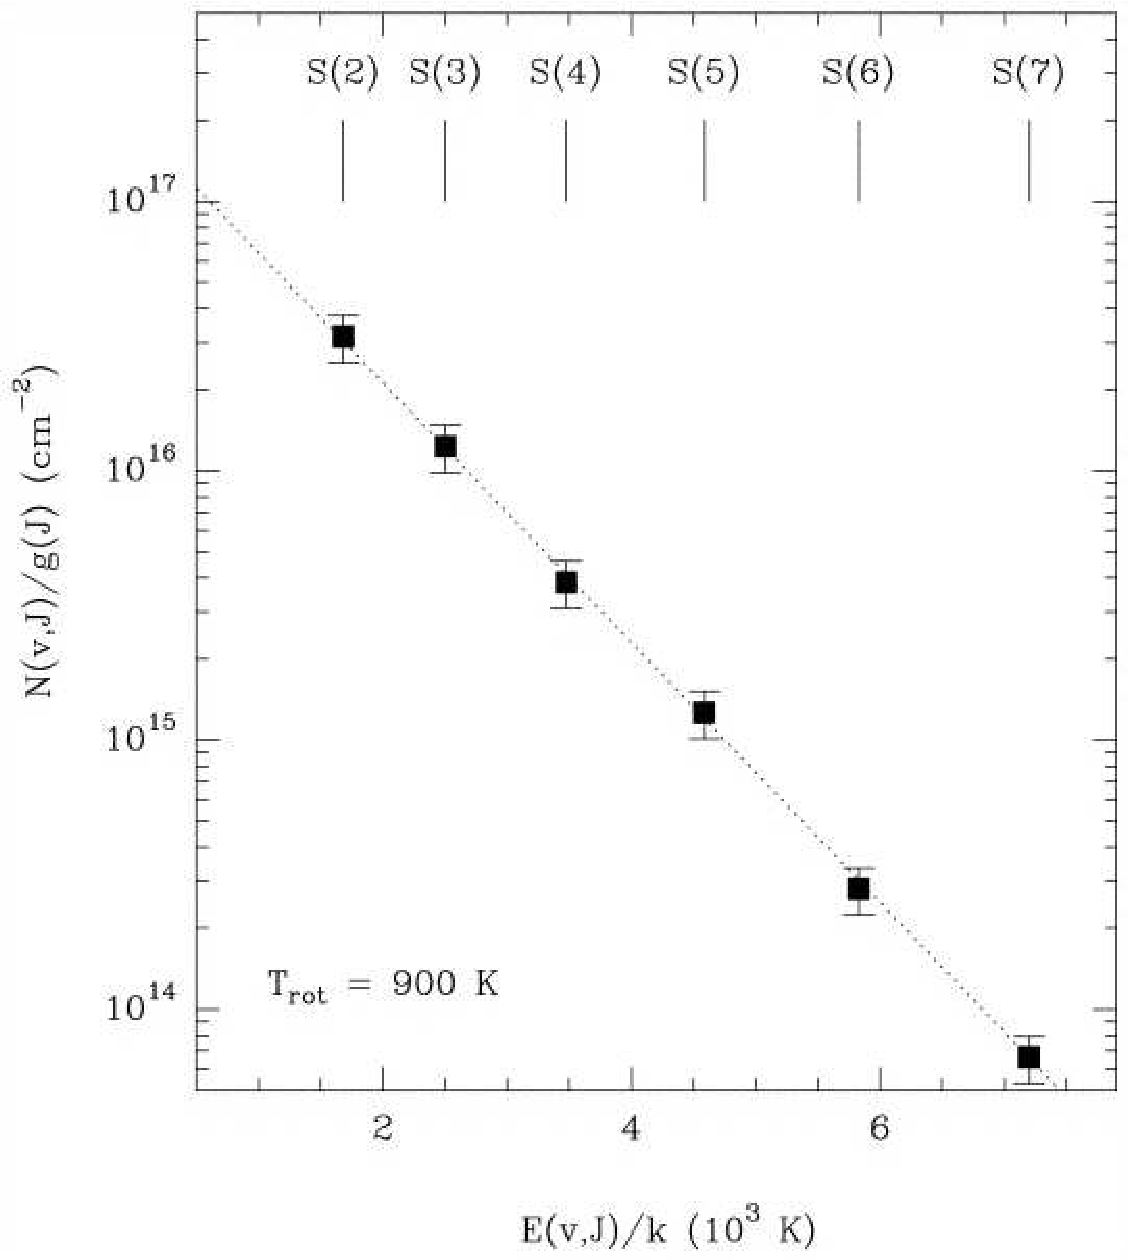
\includegraphics[width=8cm,height=8cm]{./helix_ltepop.pdf}
%\end{center}
%\end{minipage}
%\vfill
%





\end{frame} 

\begin{frame}\frametitle{Dissociation of  H$_2$}

The collisional dissociation of  H$_2$,
\[\mathrm{H}_2 + \begin{array}{c}\mathrm{He}\\\mathrm{H}\\\mathrm{e}
\end{array} \rightarrow 2\mathrm{H} +  \begin{array}{c}\mathrm{He}\\\mathrm{H}\\\mathrm{e}
\end{array},\] requires temperatures of order the binding energy of  H$_2$, $4\mathrm{.}48~\mathrm{eV}/k = 52000~$K
\footnote{the  law of mass-action does not change this
result because the number of continuum states accessible to both
products and reactants is similar, in contrast with 
ionisation, which is described by the Saha equation}.

But an H$_2$ cloud is more likely to be photo-dissociated before it
reaches 50\,000~K. The dissociation continuum of H$_2$ (i.e. free
states of H+H) starts 14.7~eV above the fundamental level of H$_2$
(i.e. X$^{1}\Sigma$, para-H$_2$), while the ionization continuum (the
ejection of one electron) starts at 15.4~eV. Both continua, ionising
and dissociating, lie above 13.6~eV. In the context of a molecular
cloud surrounded by H\,{\sc i}, the H$_2$ dissociating radiation is
completely absorbed by the Lyman continuum of H\,{\sc i}.

\end{frame} \begin{frame}\frametitle{Dissociation of H$_2$}

The likeliest mechanism for H$_2$ dissociation is absorption to the
robrivational bands of excited electronic states (e.g. B o C), and
\begin{enumerate}
\item subsequent  de-excitation to dissociated levels of lower energy
 (e.g. b$^3\Sigma$), or \label{it:1mecah2}
\item  decay to the vibrational continuum of electronic state X (with
$v \ge 14$), or  \label{it:2mecah2}
\item decay to excited levels of the fundamental state and subsequent
absorption to the dissociating continuum (one order of magnitude
slower than mechanisms 1) and 2)  
%%%%%\ref{it:1mecah2} and \ref{it:2mecah2}
, Stecher\& Williams 1967, ApJ 149, L29)
\end{enumerate}
  
\end{frame} \begin{frame}\frametitle{IR emission from  H$_2$}

Since the rate of radiative transitions within the ground state
electronic level of H$_2$ is quadrupolar, the distribution of
ro-vibrational population is dominated by collisions between H$_2$
molecules. \\

If $kT \gg \Delta E_\mathrm{FIR}$, the typical energy difference between
rotational levels of ground state H$_2$, the occupation numbers of the
robrivational levels in the ground state electronic state follow LTE:
\[ N(v,J) \propto \omega(J) \exp(-B\,(J\,(J+1))/kT), \]
in which $\omega(J) = 3 \times (2J+1) $ for ortho-$H_2$, and $\omega(J)
= 1 \times (2J+1) $ for para-$H_2$. This situation (i.e. hot molecular
gas) is typical of shocks in the ISM.

In the presence of an intense UV field the IR emission of H$_2$ is
fluorescent (Black \& Van Dishoeck, 1987, ApJ, 322, 412). Fluorescence
dominates if $kT \ll \Delta E_\mathrm{FIR}$. The absorption of one UV
photon excites H$_2$ to an electronic state, leading to
photodissociation (with a 15\% probability), and to an IR cascade in
all other cases.





\end{frame} \begin{frame}\frametitle{IR emission from H$_2$}

Example excitation diagram for the Helix nebula.

\begin{center}
\includegraphics[width=0.8\textwidth,height=!]{./B/helix_ltepop.pdf}
\end{center}

\end{frame} 

\begin{frame}\frametitle{IR emission from H$_2$, $\zeta$~Oph}
\vspace{-1.5cm}
\begin{center}
\rotatebox{-90}{\includegraphics[width=0.7\textwidth,height=!]{./B/dishoeck_fig13.pdf}}

\vspace{-1.5cm}
\rotatebox{-90}{\includegraphics[width=0.4\textwidth,height=!]{./B/ZOPH_IRACrgb.pdf}}
\end{center}


%\begin{center}
%\end{center}
%
\vfill
              
%%%%%%%%%%%%%%%%%%%%%%%%%%%%%%%%%%%%%%%%%%%%%%%%%%%%%%%%%%%%%%%%%%%%%%%%%%%%%%%%%%
%%%%%%%%%%%%%%%%%%%%%%%%%%%%%%%%%%%%%%%%%%%%%%%%%%%%%%%%%%%%%%%%%%%%%%%%%%%%%%%%%%
%%%%%%%%%%%%%%%%%%%%%%%%%%%%%%%%%%%%%%%%%%%%%%%%%%%%%%%%%%%%%%%%%%%%%%%%%%%%%%%%%%

\end{frame}


\subsection{Heating of the ISM}

 \begin{frame}\frametitle{Heating of the neutral ISM}

H$_2$ is an important source of UV opacity, as shown in the {\em FUSE}
spectra of HD210839 and HD154368 (Rachford et al., 2002, ApJ, 577,
221).

\includegraphics[width=\textwidth,height=!]{./B/fuse_H2}
\vfill

\end{frame} \begin{frame}\frametitle{Heating mechanisms}

\begin{enumerate}

\item Photoionisation: 
\[A ~  + ~h\nu ~\rightarrow~ A^+ + e, \]
in the case of the neutral ISM, photoionisation heating is dominated
by C$^+$, with an ionization potential of 11.3~eV. The average kinetic
enery of the ejected electron is 
\[ \frac{3}{2}kT_i = \frac{\int_{\nu_i}^{\infty} (J(\nu)/h\nu) \alpha_i(\nu) h(\nu
-\nu_i) d\nu}{\int_{\nu_i}^{\infty} (J(\nu)/h\nu) \alpha_i(\nu)d\nu
 }. \]

\item Photodissociation: 
\[AB ~  + ~h\nu ~\rightarrow~ A +~ B + KE, \]
dominated by $H_2$ photodissociation.
\item collisional de-excitation (in particular for H$_2$, when  
$n(\mathrm{H}_2) > 10^4~$cm$^{-3}$).
\seti
\end{enumerate}

\end{frame} \begin{frame}\frametitle{}

\begin{enumerate}
\conti
\item photoelectric effect on dust grains. \\
The grain heating efficiency, $\epsilon_\mathrm{grain}$, defined as the
ratio between output gas heating and input UV radiation (Tielens
Chap. 3.3.1), is 
\[ \epsilon_\mathrm{grain} =  Y \times \frac{h\nu - W - \phi }{h\nu}
,\]

where the electron escape probability $Y$ is the ratio between the
e$^-$ - e$^-$ mean free path $l_e \approx 10~$\angstrom, and the
absorption depth of UV radiation, $l_a \approx 100~$\angstrom :
$Y \approx l_e /l_a$.  $W$ is the work function of the grain and $\phi
= Z \times e^2 / a$ is the surface potential for a grain of size
$a$. The ionization potential of a grain is thus $ I = W + \phi$. \\
The heating efficiency is larger for smaller grains, since
$l_a \approx l_e$.  {\large The ejection of photoelectrons from grains
is the dominant heating source in the neutral ISM exposed to FUV
radiation, as in the case of PDRs. Photoionisation is dominant in the
case of the ionised gas.}
\seti
\end{enumerate}


\end{frame} \begin{frame}\frametitle{}

\begin{itemize}
\item The total photoelectric  heating  rate from grains per unit volume, $n\,\Gamma_\mathrm{grain}$, can be written:
\[ n\,\Gamma_\mathrm{grain} = \int_{a_\mathrm{min}}^{a_\mathrm{max}}
n(a) da \sum_i \int_{\nu_i}^{\nu_\mathrm{H}} \frac{J_\nu}{h\nu}
\alpha_\mathrm{grain,i}(\nu) E_\mathrm{kin}(a,i) d\nu   , \]
where $a$ is grain diameter, and $i$ runs over grain ionisation stage,
and $ h \nu_\mathrm{H} = 13.6~$eV.

\item in addition to photo-electric heating, grains can also heat the
gas through inelastic collisions if the solid state temperature is
larger than the gas temperature. 
\end{itemize}
 

\end{frame} \begin{frame}\frametitle{}


\begin{enumerate}
\conti
\item heating from cosmic rays:\\
Important for molecular phase. Cosmic rays, as well as X-rays, ionise H$_2$ (IP=15.4~eV):
\[ \mathrm{H}_2 + (p,e^-,\alpha,X) \rightarrow \mathrm{H}_2^+ + e^- +  (p,e^-,\alpha,X)^\prime,
\]
followed by the formation of $\mathrm{H}_3^+$:
\[ \mathrm{H}_2^+ +   \mathrm{H}_2 \rightarrow \mathrm{H}_3^+ + \mathrm{H}. \]
An important mechanism for the destruction of H$_3^+$ is its
dissociative recombination,
\[ \mathrm{H}_3^+ + e \rightarrow \left\{ \begin{array}{c} 3\mathrm{H} \\
  \mathrm{H}_2 + \mathrm{H} \end{array} \right. \] Since both the
  formation and the destructionof H$_3^+$ are exothermic (the energy
  released into the ISM in the process is 11~eV), the 
  H$_3^+$ cycle is a heating source of the ISM.
\seti
\end{enumerate}

\end{frame} \begin{frame}\frametitle{}


\begin{enumerate}
\conti
\item Turbulent heating.

Important in molecular clouds at $\sim 10~$K, without UV field. 


In a turbulent flow the kinetic energy density will trickle down a
hierarchy of scales, until it is dissipated by diffusion at the
smallest scale fixed by viscosity. The timescale for downwards energy
transfer at scale $l$ can be approximated with the crossing time at
the velocity disperson $v$. Thus the rate of heating per unit volume
is (Tielens 3.8),
\[ n \Gamma_\mathrm{turbulence} = \frac{1}{2} \frac{n ~ m_\mathrm{H}
v^2}{l/v} . \]

The observations of the energy density and velocity dispersion at a
given scale $l$ leads to an estimate of turbulent heating. 

The energy densities as a function of scale can be calculated assuming
a constant energy transfer rate: $ v^2 / (l/v)$ is constant. 
\seti
\end{enumerate}

\end{frame} \begin{frame}\frametitle{Heating mechanisms in neutral diffuse clouds}

\rotatebox{0}{\includegraphics[width=0.9\textwidth,height=!]{./B/heating_DC.png}}

\end{frame} \begin{frame}\frametitle{Heating mechanisms in WNM}

\rotatebox{0}{\includegraphics[width=0.9\textwidth,height=!]{./B/heating_WNM.png}}

\end{frame} \begin{frame}\frametitle{Heating mechanisms in molevular clouds}

\rotatebox{0}{\includegraphics[width=0.9\textwidth,height=!]{./B/heating_MC.png}}

\end{frame} \begin{frame}\frametitle{Steady state temp. for HI}

\rotatebox{0}{\includegraphics[width=0.8\textwidth,height=!]{./B/temp_nh.png}}

\end{frame} \begin{frame}\frametitle{Two phases for HI}

\rotatebox{0}{\includegraphics[width=0.8\textwidth,height=!]{./B/temp_p.png}}

\end{frame}

\section{Molecule formation}

\subsection{Grain catalysis}

\begin{frame}\frametitle{Molecule formation}



The encounter of two atoms $A$ and $B$, initially unbound, will lead
to molecular synthesis if:
\begin{enumerate}
\item bound states of $AB$ exist.

\item There is a mechanism for molecular stabilization faster than the
lifetime of the $AB^\star$ state \footnote{the molecule is initially
bound at a level with energy equal to that of the colliding pair}, of
order  $\sim 10^{-13}$~s ($\approx 1$ vibrational period).
\end{enumerate}


Radiative dissipation of the energy excess of $AB^\star$ is
improbable: even for electric dipole decay rates, about
$10^8~$s$^{-1}$ in the UV, only 1 out of $10^5$ collisions will produce
a molecule.\\  

The abundance of H$_2$ might raise the low probability of condensation
via collisions, but the electric dipole transitions of H$_2$ are
fobbiden. H$_2$ cannot associate radiatively.\\

The H$_2$ half-life in the diffuse interstellar UV radiation field is
of $\sim 300~$yr $\Rightarrow$ some other mechanism must exist for
efficient H$_2$ formation. 


\end{frame} \begin{frame}\frametitle{Grain catalysis of the formation process of  H$_2$}

The adsorption of hydrogen atoms onto the surface of dust grains
allows raising the available timescale for the $A$~+~$B$ encounter,
and the grain acts as stabilizing agent by absorbing the excess energy
of $AB^\star$. 

Once H$_2$ is formed, its 4.48~eV of binding energy (the first
bound-free transition is at 2500~\angstrom) eject H$_2$ from the grain
surface, and the excess of energy over the grain work function is
distributed over the molecular degrees of freedom, leaving the H$_2$
molecule in an excited state. 


IR transitions from the formation pumping of excited levels of H$_2$
were observed by Burton et al. (2002, MNRAS, 333, 721) in M~17: the
line (6-4)O(3) at 1.73$\mu$m cannot be collisionally excited since its
superior level is at $\Delta E/k$$\sim$30\,000~K above ground, yet the
intensity of (6-4)O(3) relative to other H$_2$ lines does not match
fluorescent models.

\end{frame} 

\subsection{Ion-molecule chemistry}

\begin{frame}\frametitle{Molecule formation - the
role of H$_3^+$}

$\bullet$ H$_3^+$ controls the ionisation stage of the molecular ISM. \\

The  H$_3^+$  cycle with corresponding rates is:
\[ \mathrm{H}_2 + (p,e^-,\alpha,X) \stackrel{\zeta}{\rightarrow}
\mathrm{H}_2^+ + e^- +  (p,e^-,\alpha,X)^\prime, \]
\[ \mathrm{H}_2^+ +   \mathrm{H}_2 \stackrel{\eta_1} {\rightarrow} \mathrm{H}_3^+ + \mathrm{H}, \]
\[ \mathrm{H}_3^+ + e \stackrel{\eta_2}{\rightarrow}    \mathrm{H}_2 +
\mathrm{H}, \]
where $\zeta$ is the ionization rate of H$_2$, in s$^{-1}$. We see that  
\[ \zeta n_{\mathrm{H}_2} = \eta_1 n_{\mathrm{H}_2}
n_{\mathrm{H}^+_2}, \text{~and} \] 
\[ \eta_2 n_{\mathrm{H}_3^+} n_e =  \zeta n_{\mathrm{H}_2}   \] 
With canonical values for the rates $\eta_i$, one gets
$n_{\mathrm{H}_3^+} \gg n_{\mathrm{H}_2^+}$, and the requisite for
neutrality $n_\mathrm{e} \approx n_{\mathrm{H}_3^+}$ allows concluding
$n_\mathrm{e} / n_{\mathrm{H}_2} \approx 10^{-8}~$.


\end{frame} \begin{frame}\frametitle{Ion-molecule chemistry}


$\bullet$ In ion-molecule chemistry, the standard model for
interstellar chemistry, H$_3^+$ is cornerstone to all reaction cycles:
\\ 

The cycle of an element X (anything short of He, O$_2$,...)  is 
initiated  by H$_3^+$ through 
\[ \mathrm{H}_3^+ + \mathrm{X} \rightarrow \mathrm{XH^+} + \mathrm{H}_2,~
\text{and subsequently,}\]
\[ \mathrm{XH^+} + \mathrm{Y} \rightarrow \mathrm{XY}^+ + \mathrm{H}
.\]

Example: production of $\mathrm{H_2O}$ and OH, \\
\[ \mathrm{H}_3^+ + \mathrm{O} \rightarrow \mathrm{OH^+} + \mathrm{H}_2,~
\text{followed by the sequence,}\]
\[ \mathrm{OH^+} + \mathrm{H}_2 \rightarrow \mathrm{OH_2}^+ +
\mathrm{H},  \]
\[ \mathrm{OH_2^+} + \mathrm{H}_2 \rightarrow \mathrm{OH_3}^+ +
\mathrm{H}, \]
 and finally one dissociative recombination  
\[ \mathrm{OH_3}^+ + \mathrm{e} \rightarrow \left\{ \begin{array}{l}
  \mathrm{H_2O} + \mathrm{H}\\ \mathrm{OH} + \mathrm{H_2} \end{array} \right. . \]




\end{frame} \begin{frame}\frametitle{The full story} 

$\bullet$  Molecular formation: realistic cycles (Sternberg \& Dalgarno 1995, ApJSS, 99, 565).


\begin{center}
\includegraphics[width=0.6\textwidth,height=!]{./B/C_network_2.jpg}
\end{center}

\end{frame}

\subsection{Observational validation}

 \begin{frame}\frametitle{Molecular formation - validation of
the ion-molecule chemical model}

\begin{minipage}[t]{0.48\textwidth}
H$_3^+$, the pilar of chemical cycles in the ISM, was detected by
Geballe \& Oka (1996, {\em Nature}, 384, 334; Geballe 2000, {\em
Phil.Trans.R.Soc.Lond.}A, 358, 2503), with an abundance close to that
expected from the ionization fraction.

H$_3^+$ does not have electric dipole moments, and is even worse than
H$_2$: it is deprived of excited electronic states (i.e. no UV
transitions). It only has two vibration modes. One is symmetrical,
$\nu_1$, that does not induce electric dipole moment and does not
radiate. Only the asymmetrical mode $\nu_2$ induces an electric dipole.

\end{minipage}
\hfill
\begin{minipage}[t]{0.5\textwidth}
  \vspace{-0cm}
  \begin{center}
    \includegraphics[width=\textwidth,height=!]{./B/h3_levels.jpg}
  \end{center}
\end{minipage}


%\textcolor{red}{B$_3$} Formaci\'on de mol\'eculas -
%  abundancia esperada de H$_3^+$  
\end{frame} 



\begin{frame}\frametitle{The production of  H$_3^+$}

 
\[ \mathrm{H}_2 + (p,e^-,\alpha,X) \stackrel{\zeta}{\rightarrow}
\mathrm{H}_2^+ + e^- +  (p,e^-,\alpha,X)^\prime, \]
\[\mathrm{H}_2^+ +   \mathrm{H}_2 \stackrel{\eta_2} {\rightarrow} \mathrm{H}_3^+ + \mathrm{H},\]
is balanced by its destruction, mainly through
\[ \mathrm{H}_3^+ + \mathrm{CO} \stackrel{\eta_\mathrm{CO}}{ \rightarrow} \mathrm{COH^+} +
\mathrm{H}_2, \]
equating rates, one gets
\[  \zeta n_\mathrm{H_2} = \eta_\mathrm{CO} n_\mathrm{H_3^+}
n_\mathrm{CO} ,\] in which $\eta_\mathrm{CO} = 1.8~10^{-9}~$s$^{-1}$,
and $\zeta = n_\mathrm{p,X,\alpha,e^{-}} ~\eta_1 \approx
3~10^{-17}~$s$^{-1},$ gives the product of the cosmic ray density
times the ionisation rate of H$_2$. In general the relative abundances
of CO and H$_2$ are constant in the diffuse ISM (model: Lee et al.,
1996, A\&AS, 119, 111, observations: Federman et al. 1980, ApJ 242,
545), $n_\mathrm{CO}/n_\mathrm{H_2} = 1.5~10^{-4}$, so that
\[ \boxed{ n_\mathrm{H_3^+}  \approx 10^{-4}~\mathrm{cm^{-3}}, ~~\text{independent of $n_\mathrm{H_2}$}} \]
For typical densities  $n_\mathrm{H_2} \approx 10^{4}
\mathrm{cm^{-3}}$, we have $N_{\mathrm{H}_3^+} \approx 10^{-9} N_{\mathrm{H}_2}~~~ \text{!!}$




%\textcolor{red}{B$_3$} Formaci\'on de mol\'eculas -
%  detecci\'on de H$_3^+$ 

\end{frame} \begin{frame}\frametitle{Detection of H$_3^+$, Oka \& Geballe }
\begin{center}
  \includegraphics[width=\textwidth,height=!]{./B/h3_rawspec.jpg}
\end{center}

\end{frame} \begin{frame}\frametitle{}
\begin{center}
  \includegraphics[width=\textwidth,height=!]{./B/h3_discspec.jpg}
\end{center}

\end{frame} \begin{frame}\frametitle{}
\begin{center}
  \includegraphics[width=\textwidth,height=!]{./B/h3_other.jpg}
\end{center}


\end{frame}

\subsection{Chemical fractionation}

 \begin{frame}\frametitle{ Chemical fractionation: CO}


The reaction \[ ^{13}\mathrm{C}^{+} + ~^{12}\mathrm{CO}
\overset{k_1}{\underset{k_2}{\rightleftharpoons}} ~^{12}\mathrm{C}^{+}
+ ~^{13}\mathrm{CO} + \Delta E, \]is slightly exothermic: $\Delta E /
k = 35$~K. Consequently, at low temperatures ( $\lesssim 35$~K), the
isotopic ratio $^{12}$C/$^{13}$C is different in CO than in the rest
of the {\sc ism} - there is fractionation in the C isotopes.

\end{frame} \begin{frame}\frametitle{ Chemical fractionation: theory}


At constant $P$ and $T$, minimizing the free energy $G$ gives $
\sum_i \nu_i \mu_i = 0$, and allows relating the concentration of each
species involved in the reaction. For reactions in the gas phase, we
can use the chemical potential of ideal gases,
$ \mu_i = k T \ln \left[ n_i / {\mathcal{Z}_i(T)} \right]$, 
with the partition function  \[\mathcal{Z}_i(T) = \frac{h}{\sqrt{2 \pi m_i
~k\,T}} \sum_a g^a_i e^{-\xi_a/kT}, \] where the energies associated
with the internal degrees of freedom are referred to the ground
state. We get the law of mass-action (e.g. Shu~I, 7), \[
\prod_i n_i^{\nu_i} = \prod_i \mathcal{Z}_i^{\nu_i}   .\]


\end{frame} \begin{frame}\frametitle{Application to CO} 

For CO fractionation,
\[  \frac{n(^{13}\mathrm{C}^{+}) ~n(^{12}\mathrm{CO})}{ n(^{12}\mathrm{C}^{+})
  ~n(^{13}\mathrm{CO})} = e^ {- \frac{1}{kT} \left(
  \xi(^{12}\mathrm{CO}) - \xi(^{13}\mathrm{CO} ) \right)} = \exp\left(
  -\frac{\Delta E}{kT} \right) , \] where the ground state energy is  $\xi(^{12}\mathrm{CO})$.

For CO, the rates of reactions in both directions are fast, $k_1 = k_2
= 2~10^{-10}~$cm$^3$~s$^{-1}$, and for cold clouds with  $n(H_2)
\approx 10^{4}~$cm$^3$ and $n_\mathrm{CO}/n_\mathrm{H_2} \approx
10^{-4}$, the relaxation time is $\tau_\mathrm{frac} \lesssim
1000~$yr. Thus CO is enriched in $^{13}$C, at the expense of the rest
of the molecules.

The work function of a dust grain for the adsorption of CO is
$\Delta\,H\sim$900~K, and for $T \lesssim 900~$K the probability of
adsorption for grain-CO collisions is 1. Besides the vapor pressure of
CO is very high compared to typical {\sc ism} pressures (Leger, 1983,
A\&A, 123, 271). CO is expected to be substantially (of order 50\%)
condensed onto icy CO mantles on the surface of grains (Whittet et
al. 1985, MNRAS, 216, 45).



\end{frame} \begin{frame}\frametitle{}

\begin{wrapfigure}[8]{l}{0.49\textwidth}
    \vspace{-0.5cm}
\includegraphics[width=0.49\textwidth,height=!]{./B/vandishoeck_fig4_straight.jpg}
\end{wrapfigure}  \vspace{0.1cm}  We see that the isotopic ratio
$^{12}$C/$^{13}$C will be different in the dust than in the gas phase.
Additionally the C ratio in any given molecule of the gas phase will
depend on the details of the synthesis reactions. The position taken
by CO in relation to C$^+$ will determine the C ratio in the product
molecule. This result bears on the study of the chemical evolution of
galaxies, as well as on studies of molecular cloud structure based on
the optically thin isotopes.

Chemical fractionation competes with the process of selective
photodissociation.  $^{13}$CO is dissociated by interstellar UV
radiation, penetrating to deeper lying layers in the clouds than for
the main isotope, $^{12}$CO.

\end{frame}




%
\addtocounter{part}{2}

\part{Nebular Astrophysics}
%\part[III]{Nebular Astrophysics}
\begin{frame}
  \partpage
  \tableofcontents[part=3]
\end{frame}

%
%\vspace{-1cm}
%\begin{center}
%{\tt http://www.nublado.org/ }
%\end{center}
%\vspace{-1cm}
%\begin{enumerate}
%\item Atomic Processes.\\ 
%Photoionization. Collisional Ionization. Recombination. Charge
%Transfer. \label{item:processes}
%\item Ionization Equilibrium. \\ 
%Collisional Ionization in the low density limit. Photo-ionization
%equilibrium.    \label{item:equi}
%\item Thermal Balance.  \label{item:balance}
%\item Nebular models. \\ CLOUDY. Analytical models:
%pure hydrogen nebula, OTS approximation; dustry hydrogen nebula..
%Problems with OTS - need for realistic radiative transfer. Escape
%probabilities.  \label{item:models}
%\item Temperature and density diagnostics. CELs, ORLs,
% Balmer \& Paschen discontinuities. The ORL/CEL discrepancy. \label{item:diag}
%\item Detailed study: The Helix. \label{item:example}
%\end{enumerate} 
%

\section{Atomic processes}
\subsection{Photoionization}


\begin{frame}\frametitle{Photoionization}


In time-dependent perturbation theory, the rate of transition between
two states, $i\rightarrow f $, is:
\[
\frac{dP_{if}}{dt} = \frac{e^2}{h c^3 m_e^2} \sum_{\alpha = 1}^2 \int
\omega_{fi} ~\mathcal{N}_{\alpha}(\vec{k}) ~| \langle \phi_f |
e^{i\vec{k}\cdot\vec{x} } \vec{e}_{\alpha} \cdot \vec{p} | \phi_i
\rangle |^2 ~d\Omega,
\]   
where $\mathcal{N}(\vec{k})$ is the occupation number of photons in
the state corresponding to  $\vec{k}$,
with frequency  $\nu_{fi}$.

In a photoionization process the final states $f$ belong to the
continuum. The Born approximation neglects the influence of the ion on
$|\phi_f\rangle$, and for a description of the continuum we adopt a hard
box normalization, with a size  $L \rightarrow
\infty$. With  $i$ corresponding to the fundamental state of the
hydrogen atom, we obtain (Shu~I, 23),
\[
\frac{dP_{if}}{dt} \propto \omega_{fi}^{-3} \mathcal{N}(\omega),
~\text{where } \mathcal{N}(\omega) = \int d\Omega
\mathcal{N}(\vec{\omega}) .
\]

\end{frame}
\begin{frame}\frametitle{Photoionization}



The rate of absorption of ionizing photons with frequencies in the
range $[\nu,\nu+\nu]$ is $ dN_f \frac{dP_{if}}{dt} $, where $dN_f$ is
the number of free states in the corresponding range of energies,
\[ 
dN_f = \frac{V}{2\pi^3} 4\pi~k_e^2 ~dk_e,
\]
where $\vec{k_e}$ refers to the free electron.

The cross-section of ionization is defined through
\[
P_{if} dN_f =  t~\sigma_{if}(\omega) c ~\frac{\mathcal{N}(\vec{n})}{V}
 ~4\pi n^2 dn , \text{~with } \frac{d^3\vec{n}}{V} =
\frac{d^3\omega}{(2\pi)^3 c^3}.
\]
Identifying for $\sigma(\nu)$ we get
\[
\sigma(\nu) \propto \nu^{-3}  g(\nu),
\]
where $g(\nu)$ is a gaunt factor, $g(\nu) \propto \nu^{-1/2} $, in the
Born approximation, which is valid far from the ionization edge
$\nu_\circ$. $g_\nu \approx 1 $ in the vicinity of $\nu_\circ$, where
the free-particle approximation breaks down.

\end{frame}
\begin{frame}\frametitle{The Balmer Jump: photionization of hydrogen}


\begin{center}
  \includegraphics[width=\textwidth,height=!]{./C/bj_liu.jpg}
\end{center}


\end{frame}
\begin{frame}\frametitle{Photoionization of metals\footnote{Verner et al. 1996, ApJ, 465, 487. $1~b = 10^{-24}$~cm$^2$.}}






\begin{minipage}[t]{0.49\textwidth}
  \begin{center}
    \includegraphics[width=\textwidth,height=!]{./C/ci_photion.jpg}
  \end{center}
\end{minipage}
%\hfill
\begin{minipage}[t]{0.49\textwidth}
  \begin{center}
    \includegraphics[width=\textwidth,height=!]{./C/cii_photion.jpg}
  \end{center}
\end{minipage}



\end{frame}
\begin{frame}\frametitle{Photoionization of metals: hard X-rays\footnote{{\sc cloudy} manual, Hazy.}}

  \begin{center}
    \includegraphics[width=\textwidth,height=!]{./C/auger_FeI.jpg}
  \end{center}



\end{frame}

\subsection{Collisional Ionization}

\begin{frame}\frametitle{Collisional Ionization\footnote{Arnaud \& Rothenflug 1985, A\&AS, 60, 425; Arnaud \& Raymond, ApJ, 1992, 398, 394}}

%\vspace{-1cm}
\begin{eqnarray}
\text{Direct collisional ionization: }  & \mathrm{A} + \mathrm{e} \rightarrow \mathrm{A^+} + 2~\mathrm{e}   \nonumber \\ 
\text{Excitation -- auto-ionization: }  & \mathrm{A} + \mathrm{e} \rightarrow \mathrm{A^\star} + \mathrm{e}   \nonumber  \\
                                         & \mathrm{A^{\star}}  \rightarrow \mathrm{A^+} + \mathrm{e}   \nonumber  
\end{eqnarray}
\vspace{0cm}
\begin{center}
  \includegraphics[width=0.7\textwidth,height=!]{./C/colion_xsec_2.jpg} \footnote{the
  subshell contributions to D.I. are indicated}
\end{center}



\end{frame}
\subsection{Recombination}
\begin{frame}\frametitle{Radiative recombination} 

Photoionization and its inverse process, radiative recombination, are
related by the Einstein - Milne relations (e.g. Osterbrock, A1; Shu
I,75; Spitzer p104)).  The detailed balance between photon absorptions
with frequency $\nu$ and electron-ion recombinations with relative
velocity $v$ is
\[
n_\mathrm{X} ~a_\nu 4 \pi \frac{B_\nu}{h \nu} ~d\nu = n_{\mathrm{X}^+} n_e
v \sigma(v) f(v) dv~ +~ n_{\mathrm{X}^+} n_e \sigma_2(v)  B_\nu v f(v) dv,
\]
where $~\frac{1}{2} m v^2 + h \nu_T = h \nu,$ and where $f(v)$ is the
Maxwellian integrated over angles. We get (\textcolor{red}{tarea}) that
$\sigma_2 = \sigma / (2 h \nu^3 / c^2 )$, and 
\[
\sigma(v) = \frac{g}{g_{+}}   \frac{h^2  \nu^2 }{m^2 c^2 v^2} a_\nu,    
\] 
where $g$ and $g_+$ are the degeneracies of  $X$
 and  $X^+$ in their fundamental levels.

\end{frame}
\begin{frame}\frametitle{$\bullet$ Collisional recombination} 

Recombination through 3 body collisions 
\[
 \mathrm{A^+} + 2~\mathrm{e}  \rightarrow \mathrm{A} + \mathrm{e}, 
\]
is important in the limit of very high densities. Note high densities
is not the domain of validity of the collisional ionization
equilibria, since these assume optically thin conditions. Rather, high
densities are simply described by the law of mass-action, as in
stellar interiors. 

But another domain of validity of 3-body collisions, applicable to the
diffuse ISM, is the case of radio recombination lines of H\,{\sc i}
(e.g. H\,109$\alpha$ at 6\,cm, see Osterbrock p97).


\end{frame}
\begin{frame}\frametitle{Dielectronic recombination}

The inverse process to excitation-autoionization is the dielectronic
recombination. For example (e.g. Osterbrock 1989) consider the
recombination of C$^{++}$ in its fundamental configuration
$1s^22s^2~^1$S through the collision with a 0.41~eV electron, which
matches the energy of C$^+$ in $1s^22p3d~^2$F. Doubly excited C$^{+}$
decays following a cascade (in practice 2 photons, through
$2s2p^2~^2$D) to the ground state $1s^22s^22p~^1$P$_{1/2}$.
Generically,
\[
\mathrm{X}^{+i+1} + e \rightarrow ~^{\star}\mathrm{X}^{+i} \rightarrow \mathrm{X}^{+i} + h\nu
\]
where $^{\star}X^{+i}$ is an autoionizing state of $\mathrm{X}^{+i}$.
This is the dominant mechanism for recombination at nebular
temperatures of $10^{4}$~K and densities (Nussbaumer \& Storey, 1983,
A\&A, 126, 75). \underline{No calculations are available for elements
heavier than Ne}.


\end{frame}


\subsection{Charge Transfer}

\begin{frame}\frametitle{Charge transfer}

(Spitzer + Osterbrock) 

\[
A  + H^+  \overset{k_1}{\underset{k_2}{\rightleftharpoons}} A^+ + H
\]
{$\bullet$ relationship between the rates of forward and reverse
reactions, $k_1$ and $k_2$}


\end{frame}
\section{Ionization equilibrium}
\subsection{Collisional ionization in the low density limit.}

\begin{frame}\frametitle{Ionization equilibrium - Collisional Ionization}


In the limit of low densities, and in the absence of external
radiation fields, the relative ionic concentrations are obtained from
detailed balance (the example is from Jordan (1969), but the
calculations from Arnaud et al. are more recent):
\[
\frac{N(X^{+(m+1)})}{N(X^{+m})} =
\frac{Q(X^{+m})}{\alpha_\mathrm{tot}(X^{+m})},
\]
where $Q$ and $\alpha_\mathrm{tot}$ are the rate coefficients for
ionization and recombinations.

\begin{center}
  \includegraphics[width=\textwidth,height=!]{./C/colion_eq.jpg}
\end{center}

\end{frame}

\subsection{Photo-ionization equilibrium}
\begin{frame}\frametitle{Ionization equilibrium - Photoionization}

The structure of a photoionized nebula in spherical symmetry can be
described by the ionization fraction of each element as a function of
nebular radius. For a blob of nebular material, the ionization balance
requires that the number of recombinations of ion X$^{+i+1}$ be equal 
to the number of photoionizations of  ion X$^{+i}$,
\begin{equation}
N(\mathrm{X}^{i+1}) N_{e} \alpha_{T} = {\int}d{\nu} \frac{4\pi J_{\nu}}{h\nu}
a_{\nu} N(\mathrm{X}^{i}), 
\label{eq:ionisation_balance}
\end{equation}
where $N_{e}$ is the electron density, $\alpha_{T}$ is the total
recombination coefficient, and $a_{\nu}$ is the cross-section of
photoionization, and $J_{\nu}$ is the local angular average of the
nebular specific intensity field, 
\begin{eqnarray}
J_{\nu}  & =  & \frac{1}{4~\pi}\int_{4 \pi} I_\nu d\Omega , \nonumber \\
 & = & \frac{1}{2}\int_{-1}^{+1} d\mu ~I_\nu(r,\mu), \text{~for
 spherical symmetry, with } \nonumber  \\ 
\mu &  =  & \cos \theta, \nonumber
\end{eqnarray}
where the angle   $\theta$ is measured
 relative to the radial direction.

\end{frame}
\section{Thermal Balance}
\begin{frame}\frametitle{Thermal Balance}

(R.E. Williams, en Lecture Notes on Introductory Theoretical
Physics). 

The electron bath is the specie that thermalizes fastest in an ionized
nebula (Spitzer, Cap. II). We consider the energy balance of the electrons.

$\bullet$ {\bf \large Heating of the  electrons}.
\begin{itemize}
\item collisional de-excitation. Important in dense nebulae, and
partially compensated by collisional excitations.
\item photoionization. 
\end{itemize}

\end{frame}
\begin{frame}\frametitle{Thermal Balance
- Photoionization}

Each photoelectron yields $\frac{1}{2} m v^2 = h \nu - I $ to the
electron bath, 
\[ 
G = N_\mathrm{H} \int_{\nu_1}^{\infty} 4 \pi J_\nu a_1(\nu) h (\nu -
\nu_1) d\nu  = N_\mathrm{H} \int_{\nu_1}^{\infty} 4 \pi J_\nu a_1(\nu) h (\langle
\nu \rangle  - \nu_1) d\nu,
\]
with
\[
h\langle \nu \rangle = \int_{\nu_1}^{\infty} \frac{J_\nu}{h\nu}
a_1(\nu) h \nu d\nu  / \int_{\nu_1}^{\infty} \frac{J_\nu}{h\nu} a_1(\nu)  d\nu.
\]
To a good approximation,   $a_\nu = a_\circ (\nu_1/\nu)^3$, and in the
UV we can use the Wien limit for blackbody radiation:
\[
J_\nu  \propto \nu^3 \exp \left( - \frac{h \nu} {k T_\star} \right). 
\]
\[\Rightarrow h \langle nu \rangle = \int_{\nu_1}^{\infty}
e^{-\frac{h\nu}{kT_\star}} d\nu / \int_{\nu_1}^{\infty} \frac{1}{\nu}
e^{-\frac{h\nu}{kT_\star}} d\nu \approx h\nu_1 + k T_\star. \]

\end{frame}
\begin{frame}\frametitle{Thermal Balance - OTS}

In a steady state, the equation for photoionization, $\mathrm{H} + \nu \overset{k_1}{\underset{k_2}{\rightleftharpoons}} \mathrm{H}^+ + \mathrm{e}^- ,$ 
implies that 
$k_1 = k_2 $. In general the mean specific intensity field $J_\nu(\vec{r})$ contains stellar
photons, atenuated radially by nebular absorption, and photons emitted
by the nebula. The bulk of the diffuse component is composed of Lyman
continuum photons, which can be absorbed by neutral hydrogen in the
nebula.  In the {\bf On-The-Spot} approximation, the ionization
equilibrium $k_1 = k_2$,
\[
N(\text{H\,{\sc i}})  \int_{\nu_1}^{\infty} d\nu  4 \pi J_\nu a_1(\nu)  / h
\nu = N_e N(\text{H\,{\sc ii}}) \alpha, 
\]
where  $\alpha$ is the total recombination coefficient, can be written
\[
N(\text{H\,{\sc i}})  \int_{\nu_1}^{\infty} d\nu  4 \pi J^\star_\nu a_1(\nu)  / h
\nu = N_e N(\text{H\,{\sc ii}}) \alpha^{(2)}, 
\]
where $\alpha^{(2)} = \alpha - \alpha_1$.

\end{frame}
\begin{frame}\frametitle{Thermal Balance - net heating}


The cross-section for radiative recombinations is characteristic of
Coulomb interactions,  $\propto 1/v^2$, 
\[
\sigma_\mathrm{rec} = \sigma_\circ (v_\circ/v)^2, 
\]
which follows from Milne's relation $\sigma_\mathrm{rec}(v) \approx \nu^2
a_\nu / v^2$, where $ h \nu = \frac{1}{2} m v^2 + h \nu_T \approx h
\nu_T,$ for $T_e < 10^5~$K.   Averaging over velocities, 

\[
\alpha^{(2)} =  \langle v \sigma_\mathrm{rec} \rangle \propto
 \langle  \frac{1}{v}   \rangle \propto 1/\sqrt{T_e}.
\]

Since the average kinetic energy per photoelectron is $kT_\star$, The
net heating is 

\[
G =  N_e N(\text{H\,{\sc ii}}) \alpha^{(2)} kT_\star .
\]

\end{frame}
\begin{frame}\frametitle{Thermal Balance - cooling}
%\foilhead{\textcolor{red}{C$_3$} Thermal Balance - cooling }

$\bullet$ {\bf \large Cooling of the electrons}.

\begin{itemize}
\item Collisional excitations.
\item Recombinations.
\end{itemize}



\underline{\bf Pure hydrogen nebula}\\

The excited levels of H are at energies that cannot be reached at
temperatures typical of photoionized nebulae, 13.6~(1-1/4)~eV
corresponds to  $T\approx 10^5~$K. $\Rightarrow$ cooling by
recombinations dominates, i.e. \[ L_R = N_e N(\mathrm{H\,{\small II}}) \alpha^{(2)} \frac{1}{2} m \langle v^2 \rangle \propto
\sqrt{T_e}.
\]
$\Rightarrow$ For a pure hydrogen nebula, $T_e = \frac{2}{3}
k T_\star$. 


\end{frame}
\begin{frame}\frametitle{Thermal Balance - cooling by metals}


\underline{\bf Nebulae with metals}\\

The collisional excitation of the fine structure levels (but also with
$\Delta L$) of heavy ions, such as S, N, O, C, are close to the ground
state, at only $\chi
\lesssim 3$~eV. Collisional excitation followed by radiative
de-excitation is the main cooling mechanism for ionized nebulae:
\[
L_C = N_e N(X^i) \langle \sigma_e v \rangle  \chi, 
\]
with
\[
\langle \sigma_e v \rangle  =  \frac{1}{\sqrt{T_e}} \exp( - \frac{\chi}{kT_e}). \]


\end{frame}
\section{Nebular models}
\begin{frame}\frametitle{Nebular models}

The abundance ratios of consecutive stages of ionisation,
$Q_{\mathrm{X}^{i}}=N(\mathrm{X}^{i+1})/N(\mathrm{X}^{i})$, is given
by the ionisation equilibrium:
\begin{equation}
N(\mathrm{X}^{i+1}) N_{e} \alpha_{T} = {\int}d{\nu} \frac{4\pi J_{\nu}}{h\nu}
a_{\nu} N(\mathrm{X}^{i}), 
\end{equation}
provided the ionising field is known. 
  

%Note that if the ionising potential of X$^{+i}$ is higher than the
%second ionisation energy of helium, $h\nu > 54 eV$, and if the nebula
%is optically thin at $\nu$, a guess at the outer radius of the nebula
%allows an estimate of the volume average of $Q_{X^{i}}$. Unfortunately
%what is observable is the ratio of the volume averages of the ionic
%abundances.

Given the density field, the structure of a photoionised nebula is
computed numerically by progressing outwards in radius. This is the
basic principle of the photionisation code {\small CLOUDY}, by Gary
Ferland et al.. Comparing model and observations of ionic line fluxes
is a tool for the study of nebular physical conditions. But the atomic
databases are often only approximate, and the uncertainties in the
dielectronic recombination propagate from the first stages of
ionisation.

%\foilhead{\textcolor{red}{C$_4$} Modelos de nebulosas}

\end{frame}
\begin{frame}\frametitle{High-excitation lines in PN NGC~6302}

%\bgaddcenter{\includegraphics[width=!,height=\textheight]{./C/ngc6302_Rband.pdf}}
\begin{center}
  \includegraphics[width=0.8\textwidth,height=!]{./C/specCGS4.pdf}
\end{center}

\end{frame}


\begin{frame}\frametitle{Ionization curves in NGC~6302}

%\vspace{4cm}
\begin{center}
  \includegraphics[width=0.9\textwidth,height=!]{./C/ioncurve.pdf}
\end{center}


\end{frame}
\begin{frame}\frametitle{Ionization structure in NGC~6302}

%\vspace{10cm}
\begin{center}
  \includegraphics[width=\textwidth,height=!]{./C/struct_n6302.pdf}
\end{center}


\end{frame}
\begin{frame}\frametitle{}



%\bgclear
Example input for  CLOUDY: {\tt parispn.in}\\

\medskip
\medskip
\medskip

{\tt black body, T=150,000K radius = 10\\
hden = 3.4771213\\
radius = 17\\
normalize to   Ca b  ~ 4861\\
abund he -1 C-3.523 N-4. O-3.222 ne-3.824 mg-4.523\\ 
}

\medskip

\textcolor{red}{Tarea}: Run the validation model for  CLOUDY 96 called
{\tt parispn.in}, and plot the relative abundances of each ionisation
stage for H, He and Ne. 

\end{frame}
\begin{frame}\frametitle{}

%\foilhead{\textcolor{red}{C$_4$} Modelos de nebulosas}

{$\bullet$ Str\"omgren Spheres}

{$\bullet$ Pure hydrogen nebulae}

(ver Problema 3-1 de Shu I)

{$\bullet$ Dusty H\,{\sc ii} regions.}

(Petrosian, Silk \& Field, 1972, ApJ, 177, 69; Spitzer)

{$\bullet$ Limits of the OTS approximation}.

see {\tt dhii.pdf}. 

\end{frame}
\begin{frame}\frametitle{3~D}

Monte Carlo methods allow calculating the 3D photoionisation structure
given a proton density field. The best 3D code available is Mocassin
(Ercolano et al. 2003, MNRAS, 340, 1136). 
\begin{center}
  \includegraphics[width=0.7\textwidth,height=!]{./C/MyCn18_mocassin.jpg}
\end{center}


\end{frame}
\section{Temperature and density diagnostics}
\subsection{Recombination lines}
\begin{frame}\frametitle{Temperature
and density diagnostics}


{$\bullet$ \bf Recombination lines of  H\,{\sc i}, He\,{\sc
ii}, and He\,{\sc i} } \\

The flux of a hydrogen recombination line in the optical is $F_{ij} =
\int ds d\Omega j_{ij}$, where the emissivity of a transition  $n_i
\leftarrow n_j$ populated by the recombination cascade is 
\[ 
j_{ij} = \frac{h \nu}{4 \pi} \sum_{L_i=0}^{n-1} \sum_{L_j=L_i\pm1} N_n
h\nu_{ij}.
\]
The occupation numbers $N_n$ can be calculated, and bear a weak
dependence on ${T_e,N_e}$. The radiative transfer effects are included
through an OTS approximation that distinguishes two cases (Baker \&
Menzel 1938, ApJ, 88, 52): case A, where the nebula is optically thin
in every transition (as well as in the Lyman continuum), and case B
where all photons from the Lyman serie, as well as the Lyman
continuum, are absorbed OTS, so that the effective fundamental state
in the recombination cascade is $n=2$.

\end{frame}
\begin{frame}\frametitle{Optical Recombination Lines - ORLs}



%\foilhead{\textcolor{red}{C$_5$} L\'{\i}neas de recombinaci\'on}

The effective recombination coefficient is defined through 
\[
N_p N_e \alpha_{ij}^\mathrm{eff} = \frac{4 \pi}{h \nu_{ij}}  j_{ij}.
\]
Hummer \& Storey (1987, MNRAS, 224, 801) give 
$\alpha_\mathrm{H\beta}^\mathrm{eff} =3.0~10^{-14}~$cm$^{-3}$, at
$10^4$~K (approximately  $\propto
\sqrt{1/T_e}$), and tabulate the emissivities of H\,{\sc i} and
He\,{\sc ii} recombination lines relative to $H_\beta$. The relative
emissivities for the He\,{\sc i} recombination lines are tabulated by
Smits, MNRAS, 251, 316. Those of O\,{\sc ii}, N\,{\sc ii}, N\,{\sc
iii}, Ne\,{\sc ii}, C\,{\sc ii} y C\,{\sc iii} have been computed by
Storey et al. and can be found in the recent literature.

Note that given $N_e$ and the flux of a recombination line, it is
straightforward to obtain the column of the corresponding ion. For
example the recombination spectrum of O\,{\sc ii} gives the column of
O$^{2+}$, which has the spectrum of O\,{\sc iii}.

\end{frame}
\subsection{Collisionally Excited Lines - CELs.}
\begin{frame}\frametitle{Collisionally Excited Lines - CELs.}


%\foilhead{\textcolor{red}{C$_5$} L\'{\i}neas excitadas por colisiones - CELs.}

The flux of an optically thin CEL $i \leftarrow j$ is given by
integrating the line emissivity along the optical path $s$:
\[
F_{ij} = \int ds \int d\nu \, d\Omega ~ j_\nu = \int ds \, d\Omega ~ \frac{
A_{ij}\, h\nu_{ij}}{4\pi}~ N_j ,
\]
where  $N_j$ is the population of the excited level $j$.

% and where $b$
%is the ``branching ratio'', in the general case where there is more
%than one transition branching off the same upper level: $b = A_{ij} /
%\sum_{k<j} A_{kj}$.

The principle underlying the diagnostic of physical conditions in
ionised nebulae is the dependence of $N_j(\vec{r})$ on
$T_e,N_e$. Neglecting radiative excitations (i.e. optically thin case),
\[
\sum_{i{\neq}j}
{n}_{j}{C}_{ji} +
\sum_{i<j}{n}_{j}{A}_{ji} = \sum_{i{\neq}j}{n}_{i}{C}_{ij}  + \sum_{i>j}{n}_{i}{A}_{ij}, 
\]
where $N_j = n_j \, N_\circ$, and $N_\circ$ is the ground state
population. In LS coupling the Hund rules give 2 to 5 levels in the
fundamental configuration of common ions. 

\end{frame}
\subsection{Temperature and density.}
\begin{frame}\frametitle{Density-sensitive pairs of  lines}

%\begin{minipage}[t]{11cm}
%  \begin{center}
%    \includegraphics[width=10cm,height=!]{oii.pdf}
%  \end{center}
%\end{minipage}
%%\hfill
%\begin{minipage}[t]{15cm}

\begin{wrapfigure}[10]{l}{0.49\textwidth}
    \vspace{-0.5cm}
\includegraphics[width=0.49\textwidth,height=!]{./C/oii.pdf}
\end{wrapfigure}  \vspace{0.1cm}  The critical densities of both lines are 
 $N_c(\lambda3729) = 4\,10^{13}$cm$^{3}$ and $N_c(\lambda3726) =
2\,10^{4}$cm$^{-3}$, both comparable to typical nebular densities. The
ratio of these lines does not depend on the concentration of
O$^+$. Since the upper levels are very close in energy, their relative
populations are insensitive on temperature. The [O\,{\sc ii}] doublet
is a good diagnostic for densities close to the critical densities.

\end{frame}
\begin{frame}\frametitle{density}


[O\,{\sc ii}] doublet for typical densities:
\begin{itemize}
\item $N_e \ll N_c$. \[ \frac{I(\lambda 3279)}{I(\lambda 3726)} =\frac{ N_e
N_1  \langle \sigma_{12} v \rangle \frac{h\nu_{21}}{4\pi}}{ N_e
N_1  \langle \sigma_{13} v \rangle \frac{h\nu_{31}}{4\pi}} = \frac{ \langle
\sigma_{12} v  \rangle}{\langle \sigma_{13} v  \rangle},\] independent
of $N_e$\footnote{and also of  $T_e$ because  $\sigma \propto g$ for
fine structure levels}
\item $N_e \gg N_c$. In this case  $N_3 = N_1 C_{13}/C_{31} = N_1 g_3
e^{-\chi_3/kT} / g_1 $  and 
\[\frac{I(\lambda 3279)}{I(\lambda 3726)} = \frac{A_{21}
N_2 g_2 }{A_{31}N_3 g_3}, \] independent of  $N_e$ and weakly
dependent on $T_e$.
\item In an intermediate case, we consider  $N_c(\lambda 3729) \ll N_c
\ll N_c(\lambda 3726)$:
\[\frac{I(\lambda 3279)}{I(\lambda 3726)} = \frac{g_2}{g_3}
\frac{A_{21}}{N_e \langle \sigma_{12} v \rangle} \propto
\sqrt{T_e}/N_e,\]  which is a function of  $N_e$.
\end{itemize}

%\end{minipage}

\end{frame}
\begin{frame}\frametitle{Temperature-sensitive pairs}

%\begin{minipage}[t]{8cm}
%  \begin{center}
%    \includegraphics[width=7cm,height=!]{oiii.pdf}
%  \end{center}
%\end{minipage}
%    \includegraphics[width=7cm,height=!]{oiii.pdf}
%\hfill
%\begin{minipage}[t]{15cm} 
%\vspace{-8cm}


\begin{wrapfigure}[12]{l}{0.39\textwidth}
    \vspace{-0.5cm}
\includegraphics[width=0.39\textwidth,height=!]{./C/oiii.pdf}
\end{wrapfigure} These 3 transitions have $A \gtrsim 1$~s$^{-1}$,  $N_c \gg
10^{4}$~cm$^{-3}$, and $A_{32} \ll A_{31}$, so that 
\begin{eqnarray}
j(\lambda4363) & = &  N_e N_1 \langle \sigma_{13} v \rangle \frac{h \nu_{32}}{4\pi}, \nonumber \\
j(\lambda5007) & = &  N_e N_1 \left[ \langle \sigma_{12} v \rangle  + \right. \nonumber   \\
 &&   \left. \langle \sigma_{13} v \rangle  \frac{A_{32}}{A_{31}+A_{21}} \right] \frac{h \nu_{21}}{4\pi},  \nonumber 
\end{eqnarray}
where we have treated  $\lambda4959$ and $\lambda5007$ as a single
line. The ratio of these  {\bf two} lines is 
\[
\frac{I(\lambda 5007)}{I(\lambda4363)} = \frac{\lambda_{32}}{\lambda_{21}}
\left[1+\frac{\langle \sigma_{12} v \rangle}{\langle \sigma_{13} v
\rangle } \right].
\]
Remembering that  $\langle \sigma_{ij} v \rangle \propto T_e^{-1/2}
e^{-\chi_{ij}/kT_e}$, we see that the ratio $\frac{I(\lambda
5007)}{I(\lambda4363)} $ is sensitive on the temperature. One gets 
$I(\lambda 5007)/I(\lambda4363) \approx 8~\exp(33000/T_e)$.

%\end{minipage}


\end{frame}
\begin{frame}\frametitle{Density and the ORLs}

%
%\begin{wrapfigure}[8]{l}{0.49\textwidth}
%    \vspace{-0.5cm}
%\includegraphics[width=0.49\textwidth,height=!]{./C/Hn_Ne.jpg}
%\end{wrapfigure}   The recombination lines have a very weak
%dependence on density, which can be used as diagnostic (Liu et
%al. 2000, MNRAS, 312, 585).
%

\begin{center}
\includegraphics[width=0.55\textwidth,height=!]{./C/Hn_Ne.jpg}
\end{center}   

The recombination lines have a very weak dependence on density, which
can be used as diagnostic (Liu et al. 2000, MNRAS, 312, 585).


\end{frame}
\subsection{The line-continuum-temperature relationship }
\begin{frame}\frametitle{The line-continuum-temperature relationship   }


The radio-continuum flux density of free-free radiation relates to the
H$\beta$ flux through
\[
F(H\beta) = 0.28 T_e^{-0.52} \nu^{0.1} F_\nu,
\]
which gives $T_e$. The recombination lines with $n\gg 1$ at radio
frequency are not extinct, and their emissivities can be calculated in
LTE (the correction is $\ll 1$ and is tabulated by Brocklehurst 1970,
MNRAS 148, 417).


\end{frame}
%\subsection{Balmer and  Paschen discontinuity }

\begin{frame}\frametitle{Balmer and  Paschen discontinuity   }

\vspace{0cm}
\begin{minipage}[t]{0.48\textwidth}
$BJ = \frac{I_c(\lambda3643)-I_c(\lambda3681)}{I(H11,\lambda3770)}.$
\\ $I_c(\lambda)$ is tabulated by Brown \& Mathews (1970, ApJ, 160,
939).

\begin{center}
  \includegraphics[width=0.9\textwidth,height=!]{./C/bj_liu.jpg} \end{center}
\end{minipage}
%\hfill
%\vspace{6cm}
\begin{minipage}[t]{0.48\textwidth}
\vspace{-0.5cm}
  \begin{center}
    \includegraphics[width=0.9\textwidth,height=!]{./C/BJ_T.jpg}
  \end{center}

He$^+$/H$^+$ = 0.1, He$^{++}$/H$^+$=0 (dots);
He$^+$/H$^+$ = He$^{++}$/H$^+$=0.05   (solid);
He$^+$/H$^+$ = 0, He$^{++}$/H$^+$=0.1   (dashed).

\end{minipage}

\medskip

The same analysis can be applied to the Paschen discontinuity at
8194\AA.

\end{frame}
\subsection{The ORL/CEL discrepancy}
\begin{frame}\frametitle{The ORL/CEL discrepancy }

\begin{center}
      \includegraphics[width=0.9\textwidth,height=!]{./C/ORL_CEL_general.jpg}
\end{center}


\end{frame}
\begin{frame}\frametitle{ORL/CEL}

\begin{itemize}
\item In principle the best indicators of ionic abundances are the
ORLs, because the recombination coefficients of both hydrogen and
metals are approx. $\propto 1/\sqrt{T_e}$, so that the residual
dependence on temperature is very weak.

\item The difficulty with  ORLs is that their fluxes are  $10^{-3} -
10^{-4}$ weaker than H$\beta$.

\item By contrast the CELs have an exponential dependence on
temperature, and their fluxes are comparable to H$\beta$.

\end{itemize}

\end{frame}
\begin{frame}\frametitle{ORL/CEL}

\begin{center}
      \includegraphics[width=\textwidth,height=!]{./C/orl_cel_table.jpg}
\end{center}

There is a systematic discrepancy between CELs and ORLs:\begin{itemize}
\item $T_e(\mathrm{CEL}) > T_e(\mathrm{ORL} \sim T_e(\mathrm{continuum})$
 
\item $N(X^{+i})(\mathrm{CEL}) < N(X^{+i})(\mathrm{ORL})$, although
the columns are similar when using the same temperatures.
\end{itemize}

\end{frame}
\begin{frame}\frametitle{ORL/CEL discrepancy  -
temperature fluctuations.  }

One strategy to reconcile the temperature discrepancy, original
proposed by Peimbert (1967, ApJ, 150, 825) to explain the systematic
discrepancy in $T($O\,{\sc iii}) and $T(\mathrm{continuum})$, is the
``$t^2$'' formalism. In this formalism one expands the CEL emissitivies
in small temperature fluctuations about a mean value:
\[
j(T) = j(T_\circ) + (T-T_\circ)
\left. \frac{dj}{dT}\right|_{T=T_\circ} + \left. \frac{1}{2} (T-T_\circ)^2
\frac{d^2j}{dT^2}\right|_{T=T_\circ}, \text{and,}
\]
\[
\int N_e N_i j(T) ds = j(T_\circ) \int N_i N_e ds + \left. \frac{1}{2}
\frac{d^2j}{dT^2}\right|_{T=T_\circ} \int ds N_i N_e (T-T_\circ)^2,
\]
where the term of order 1 cancels out when choosing\[
T_\circ = \int ds N_i N_e T / \int ds N_i N_e \text{. ~~We define } 
t^2 = \frac{\int N_i N_e (T-T_\circ)^2 ds}{T_\circ^2  \int
ds N_i Ne }.\]

Two pairs of $T_e$-sensitive lines allow calculating $T_\circ$ and
$t^2$. In this formalism $T_\circ$ is {\bf the }  nebular temperature,
and is closer to the ORLs and to the continuum than to the CELs. In
other words $t^2$ effectively adopts the ORL values. 

\end{frame}
\begin{frame}\frametitle{ORL/CEL discrepancy - solution?}

An alternative to the $t^2$ formalism is to interpret the observed
discrepancies as real, and conclude there are cold and metal rich
inclusions in the nebulae. These inclusions may find their origin in
the evaporation of globules or ices on big-grains (or planetesimals)
for H\,{\sc ii} regions, or in the ejection of enriched stellar
material in the dredge-up of AGB precursors to planetary nebulae.


\begin{center}
      \includegraphics[width=\textwidth,height=!]{./C/orl_cel_table.jpg}
\end{center}

\end{frame}
\begin{frame}\frametitle{ORL/CEL discrepancy - solution?}


Photoionisation models with two phases indicate that the bulk of
nebular material should come from the `hot' component, which is traced
by the CELs (good news!). A test for this interpretation is to study
the thermal broadening of the ORLs, as observed by Barlow et
al. (astro-ph/0605235), who compared [O\,{\sc iii}]~4363\AA~ with the
sum of the O\,{\sc ii} ORLs at 4089\AA, 4275\AA~ and 4349\AA:
\begin{center}
      \includegraphics[width=0.7\textwidth,height=!]{./C/n7009_bHROS.jpg}
\end{center}


\end{frame}


%
\addtocounter{part}{3}

\part{Interstellar dust}
%\part[III]{Nebular Astrophysics}
\begin{frame}
  \partpage
  \tableofcontents[part=4]
\end{frame}

\section{Extinction}

\begin{frame}\frametitle{Extinction}


References: 

Draine, B.T., 2003, ``Astrophysics of Dust in Cold Clouds'',
astro-ph/0304488
Draine, B.T., 2004, ARA\&A, 41, 241


\begin{itemize}

\item $A_\lambda \equiv -2.5 \log_{10} I_\mathrm{obs} /
I_\mathrm{int}$. 

\item $I_\mathrm{obs} = \exp(-\tau)  I_\mathrm{int}$
${\bf \Longrightarrow}$ $A_\lambda = 2.5 \tau / \ln(10) \approx 1.086
\tau(\lambda)$. 

\item $A_\lambda$ is measured by comparing magnitudes  for star with
the same spectral type, or else using recombination lines. 





\item $R_V = A_V / E(B-V)   = A_V / (B-V|_\mathrm{obs} - B-V|_\mathrm{int}) = A_V / (A_B - A_V)$

\end{itemize}

\end{frame}
\begin{frame}\frametitle{Extinction}

\begin{itemize}


\item grains $\ll \lambda$: Rayleigh-scattering gives $A_\lambda \propto
\lambda^{-4}$, $R_V \approx 1.2$. 

\item grains $\gg \lambda$: gray extinction, independent of 
$\lambda$, $R_V \rightarrow \infty$.


\item Parametrisation in terms of single parameter  $R_V$ OK for
$\lambda > 3030~$\AA:
\[ A(\lambda),R_V) = a(\lambda)  + b(\lambda) / R_V, \]
where $a(\lambda)$ and $a(\lambda)$ are power laws, set by fitting the
data (Cardelli et al., 1989, ApJ, 345, 245). 

\item For $\lambda < 3030~$\AA~, use $A_\lambda \approx f(\lambda;
R_V,\{a_i\})$ where $\{a_i\}$ charasterise the UV `bump'.

\item In the  IR, between  $0.9$ and  $6\mu\mathrm{m}$, $A_\lambda$ is $\pm$
universal: $A_\lambda = 2.4~\lambda^{-1.75}$ (Draine 1989, quoting
`Infrared Astronomy', Tokunaga in {\em Astrophysical Quantities}).

\end{itemize}


\end{frame}
\begin{frame}\frametitle{Extinction}


\begin{center}
\rotatebox{-90}{\includegraphics[width=!,height=\textwidth]{./D/draine_araa_f1.pdf}}
\end{center}


\end{frame}
\begin{frame}\frametitle{Extinction}

\begin{center}
\rotatebox{-90}{\includegraphics[width=!,height=\textwidth]{./D/draine_araa_f5.pdf}}
\end{center}


\end{frame}
\begin{frame}\frametitle{$R_V$?}



\begin{itemize}
\item Galactic bulge: $R_V = 1.8-2.5$ (Udalski 2002)
\item LMC: $R_V=3.1 $ (Udalski 2002)
\item Cirrus clouds (far from the galactic plane):  $R_V=2 $ (Guhathakurta
1999).
\item Typical value for the local  {\sc ism} : $R_V = 3.1\pm 2$!?
(Cardelli et al 1989)
\end{itemize}


\end{frame}
\begin{frame}\frametitle{$N_H \leftrightarrow A_{V}$\footnote{
ojo: $A_V$ vs $1/R_V \propto 1/A_V$}}


Using H\,{\sc i} Ly$\alpha$ and H$_2$ absorption lines to measure the
column of protons to nearby stars gives $N_H / E(B-V) = 5.8~10^{21}$
cm$^{-2}$mag$^{-1}$, or $N_H / A_V = 1.87~10^{21}$
cm$^{-2}$mag$^{-1}$, for $R_V = 3.1$. But $N_H
\leftrightarrow A_{V}$  varies with sighlines:
\begin{center}
\rotatebox{-90}{\includegraphics[width=!,height=0.6\textwidth]{./D/draine_araa_f2.pdf}}
\end{center}
$A_V(N_H)$ follows $Z$ in the Magellanic Clouds: 40\% of Milky Way
extinction in LMC, 10\% in SMC.


\end{frame}
\begin{frame}\frametitle{$A_\lambda$ over 6-8~$\mu\mathrm{m}$ }


%\vspace{-1cm}
\begin{center}
\includegraphics[width=!,height=0.8\textwidth]{./D/ISO_field_GC.jpg}
\end{center}


\end{frame}
\begin{frame}\frametitle{$A_\lambda$ over 6-8~$\mu\mathrm{m}$ }


Lutz et al. (1996, A\&A, 315, L269) find excess extinction assuming
Case B for H recombination lines in the $ISO$+SWS spectrum.
%\vspace{-1cm}
\begin{center}
\includegraphics[width=\textwidth,height=!]{./D/iso_GC.jpg}
\end{center}


\end{frame}
\begin{frame}\frametitle{$A_\lambda$ over 6-8~$\mu\mathrm{m}$ }


%\vspace{-1cm}
\begin{center}
\rotatebox{-90}{\includegraphics[width=!,height=\textwidth]{./D/draine_araa_f4.pdf}}
\end{center}


\end{frame}


\begin{frame}\frametitle{Uncertainties in $A_\lambda$}

\begin{wrapfigure}{l}{0.56\textwidth}
\includegraphics[width=0.55\textwidth, height = !]{./D/dwek_fig1.jpg}
\end{wrapfigure}  Dwek (2004, ApJL, 611, 109)
proposes that the excess extinction at $\sim$6~$\mu\mathrm{m}$ is due
to metallic needles (ref. Hoyle \& Wickramasinghe).  {\bf short dash}:
silicates, {\bf long dash}: metallic needles, {\bf dots}: graphite,
{\bf dot-dash}: PAHs, {\bf thin solid}: standard extinction.




\[
\tau(\lambda) = \sum_j \int_0^L\,ds \left[
\int_{a_{\mathrm{min},j}}^{a_{\mathrm{max},j}} da f_j(a)
\kappa_j(\lambda,a) \rho_{d,j}(a,s)\right], ~~\text{with} 
\]
\[
\int_{a_{\mathrm{min},j}}^{a_{\mathrm{max},j}}  f_j(a) = 1.
\]



\end{frame}

\begin{frame}\frametitle{NICER and $A_V$ maps}

Lombardi, Alves, 2001, A\&A 377,1023.

\begin{center}
\includegraphics[width=0.6\textwidth,height=!]{./D/lombardi_alves_NICER.jpg}
\end{center}

JHK extinction follows a fairly universal law, so JHK imaging allows
accurate near-IR extinction measurements through stellar counts.

Very useful: $A_V$ can be converted to $N_H$, and thereby to total
masses.


\end{frame}

\begin{frame}\frametitle{The UV bump: VSGs}


\begin{minipage}[t]{0.59\textwidth}
\begin{itemize}
\item The UV bump matches a Lorentzian (in truth a `Drude' profile).
\item The fitting of a Lorentzian allows infering $n_X f_X/ n_H =
9.3~10^{-6}$, and since the oscilator strength of the absorbing specie
  cannot be in excess of $\sim 1$, $f_X \lesssim 0.5$, one requires
  $n_X/n_H \gtrsim 4~10^{-5}$, allowing to consider compounds of
  $\{C,N,O,Mg,Si,Fe\}$.
\item The centre of the bump is constant at  2175\AA,  although the
  width of the bump varies with 1~$\sigma \approx 6\%$.
%\item Grafito podr\'{\i}a explicar  
\end{itemize}
\end{minipage}
\hfill
\begin{minipage}[t]{0.4\textwidth}
\vspace{-1cm}
  \begin{center}
    \includegraphics[width=\textwidth,height=!]{./D/uvbump_drude.jpg}
    \end{center}
\end{minipage}


\end{frame}
\begin{frame}\frametitle{}


\begin{minipage}[t]{0.5\textwidth}
\begin{itemize}
\item A ground state transition in the delocalized electrons of the
hexagonal benzene rings lies precisely at 2175\AA.

%\item un transici\'on al nivel excitado en los electrones
%deslocalisados de los anillos hexagonales de benzeno esta precisamente
%a 2175\AA.

\item Graphite, with  $f = 0.16$ could explain  $\lambda_\circ$, and
the absorption strength with C/H$=5.8~10^{-5}$ (OK for cosmic
abundances), but not the FWHM variations. 

\item Variations in the mixture of different PAHs molecules are
required to explain the $FWHM$ variations. 
\end{itemize}
\end{minipage}
\hfill
\begin{minipage}[t]{0.49\textwidth}
\vspace{-0.1cm}
  \begin{center}
\rotatebox{-90}{\includegraphics[width=!,height=0.6\textwidth]{./D/draine_araa_f7.pdf}}
    \end{center}
\end{minipage}


\end{frame}
\begin{frame}\frametitle{Silicate extinction}

\begin{itemize}
\item The 10$\mu$m silicate feature is seen in absorption when the
  screen is colder than the background illuminating source. It is seen
  in emission in M stars (C/O$>1$) , or in planetary nebulae with
  C/O$>1$.

\item Stretching  mode of  Si-O at 9.7~$\mu$m. 

\item Properties of silicates vary substantially with environment.

\item The extinction curve at  10$\mu$m is smooth and shows no fine
structure, in marked contrast with the crystalline silicate spectra
$\Rightarrow$ interstellar silicates are amorphous.

\item But there is a significant fraction of crystallinity in
circumstellart disks and AGB (M) star outflows.

\item Bowey et al. propose that up to  60\% of  silicate mass in dense
dark cloud is crystalline (criticised). 
\end{itemize}

 
\end{frame}
\begin{frame}\frametitle{\footnote{Bowey \& Adamson 2002, MNRAS, 334, 94}}

\begin{minipage}[t]{0.3\textwidth}
\vspace{0.5cm}
  \begin{center}
\includegraphics[width=\textwidth,height=!]{./D/bowey_spectra.jpg}
    \end{center}
\end{minipage}
\hfill
\begin{minipage}[t]{0.3\textwidth}
\vspace{-1.0cm}
  \begin{center}
\includegraphics[width=\textwidth,height=!]{./D/bowey_obs_taus.jpg}
    \end{center}
\end{minipage}
\begin{minipage}[t]{0.3\textwidth}
\vspace{-1.0cm}
  \begin{center}
\includegraphics[width=\textwidth,height=!]{./D/bowey_mod_taus.jpg}
    \end{center}
\end{minipage}
\hfill



\end{frame}
\begin{frame}\frametitle{Silicate extinction}
 


\begin{center}
      \includegraphics[width=0.6\textwidth,height=!]{./D/cristsil_bowey.jpg}
\end{center}


\end{frame}
\begin{frame}\frametitle{Variations in the silicate profiles\footnote{Van Dischoeck, 2004, AR\&AA}}

\begin{center}
      \includegraphics[width=0.9\textwidth,height=!]{./D/dishoeck_fig12.pdf}
\end{center}

\end{frame}
\begin{frame}\frametitle{Absence of crystalline silicates in the diffuse ISM\footnote{Kemper et al. ApJ 2004, 609, 826}}

\begin{minipage}[t]{0.5\textwidth}
\vspace{0.5cm}
  \begin{center}
      \includegraphics[width=0.6\textwidth,height=!]{./D/taus_ISO_GC.jpg}
      \end{center}
\end{minipage}
\hfill
\begin{minipage}[t]{0.49\textwidth}
\vspace{-0.5cm}
  \begin{center}
\includegraphics[width=\textwidth,height=!]{./D/crist_ks.jpg}
    \end{center}
$\Rightarrow$ Crystalline silicates represent $\sim~0.2\pm0.2$ by
mass. \\
Since the silicates in the AGB star outflows have high
fractions of crystallinity, there must be substantial interstellar
processing of dust in the ISM.
\end{minipage}


\end{frame}
\begin{frame}\frametitle{Ice absorption}


\begin{center}
\rotatebox{-90}{\includegraphics[width=!,height=\textwidth]{./D/dishoeck_fig7.pdf}}
\end{center}









%\foilhead{}
%\leftheader{}
%
%\begin{center}
%\includegraphics[width=\textwidth,height=!]{./D/ngc7293_3D.pdf}
%\end{center}
%




\end{frame}

\section{IR emission from dust}

\begin{frame}\frametitle{IR emission from dust}

If the grains are in steady state, their internal energy and
temperature are constant, and the emergent spectrum from a homogeneous
cloud is 
\[ 
I_\nu = B_\nu (T_d) \left[ 1 - \exp(-\tau_d) \right], 
\]
with  $\tau = \kappa(\lambda) \int \rho ds $, and
\[ 
\kappa(\lambda) = \frac{1}{1.4 n_H m_H} \int da \frac{dn}{da}
C_\mathrm{abs}(a,\lambda),
\]
where $\rho$ is the mass density (with gas), and $n(a)$ is the number
density of grains with radii $< a$. Thus the column of mass is 
\[
\int \rho ds \approx \frac{1}{\kappa(\lambda)}
\frac{I_\nu}{B_\nu(T_d)}~.
\]
The opacities $\kappa$ and cross sections $C_\mathrm{abs}$ are
tabulated in the web page of B. Draine: {\tt
http://www.astro.princeton.edu/\~draine/dust/dust.html}.

\end{frame}
\begin{frame}\frametitle{IR emission from dust}


The power absorbed by a grain is 
\[
\left.\frac{dE}{dt}\right|_\mathrm{abs} = \int_0^\infty d\nu u_\nu c
C_\mathrm{abs}(\nu),
\]
and emitted  power  is 
\[
\left.\frac{dE}{dt}\right|_\mathrm{rad} = \int_0^\infty d\nu 4\pi B_\nu
C_\mathrm{abs}(\nu).
\]
We can express $T_s$, the steady state temperature, from 
$\left.\frac{dE}{dt}\right|_\mathrm{abs} =
\left.\frac{dE}{dt}\right|_\mathrm{rad}$, {\bf under the assumption
that collisions do not contribute to the thermal blance}.

But in reality $E$, the internal energy of the grain, and $T$, its
temperature, vary stochastically, and the flutuactions are more
pronouced when $h\nu \sim E$, as is the case for very small
grains. 

%Thus one needs to determine the probability density associated
%to $E$, through a thermal balance. 

\end{frame}
\begin{frame}\frametitle{Feature at   3.4~$\mu$m: C-H 
alifatic stretch (carbon chains)}

\begin{center}
  \includegraphics[width=\textwidth,height=!]{./D/specCGS4.pdf}
\end{center}

\end{frame}
\begin{frame}\frametitle{Other dust features}

\begin{itemize}
\item Diamonds are seen in two Herbig AeBe stars and one AGB star,
  through emission bands at 3.4 and 3.5~$\mu$m due to hydrogenated
  surface impurities on an otherwise regular carbon-crystal lattice.

\item SiC (silicon carbide) is seen towards C stars and PNe. 

\item The Extended Red Emission, or a broad featureless continuum at
  6000 to 8000~\AA, is seen towards all lines of sight (i.e. cirrus
  and dark clouds, H\,{\sc ii} regions, PNe and galaxies in
  general). The carriers of ERE have yet to be identified. 


\item Fullerenes (Kroto et al. 1985, Nat, 318, 162) in post-AGB stars and PNe, e.g. Bernard-Salas et al., 2012, ApJ, 757, 41B


\end{itemize}

\end{frame}

\section{VSGs}

\begin{frame}\frametitle{VSGs}



\begin{itemize}

\item  The VSGs are necessary to explain the variations in the UV bump
of the extinction curve.


\item Andriesse (1978) postulated the VSGs to explain the variation of
the dust temperature in a cloud near M17.  $T_\mathrm{colour}$ in the
NIR and FIR are 150K y 38K, respectively, while the NIR and FIR
morphologies are practically identical $\rightarrow$ the two
temperatures are mixed, and it is necessary to postulate the
temperature excursions of VSGs (which were called Platt particles at
the time). 

\item Sellgren et al. (1983) found  that the NIR emission in
reflection nebula is extended and consists at least of one emission
band at 3.3~$\mu$m as well as a continuum with $T_\mathrm{colour} =
1000$~K, with minimal variations with distance from the central star.
Sellgren (1984, ApJ, 277, 623) noted that if the dust was in radiative
equilibrium with the star, its temperature should decrease rapidly
with distance, and so postulated the VSGs.

\end{itemize}

\end{frame}


\begin{frame}\frametitle{VSGs}

\begin{itemize}
\item The  12~$\mu$m and 25~$\mu$m emission from Galactic cirrus, 
discovered by {\em IRAS}, is much higher than that expected from large
grains in equilibrium with the local radiation field (with T$\sim
18-25~$K, Boulanger \& Perault 1988).

\item Spinning dust?

\end{itemize}

\end{frame}
\begin{frame}\frametitle{Stochastic heating of VSGs}


\begin{center}
\rotatebox{-90}{\includegraphics[width=0.5\textwidth,height=!]{./D/T_fluctuations.pdf}}
\end{center}

A grain with radius $5$~\AA (i.e. a PAH) receives 1 UV photon (10~eV)
per year in the radiation field of the solar neighbourhood. When
absorption occurs, the dust grain temperature may rise up to 1000~K.
  

%\begin{floatingfigure}{16cm}
%\includegraphics[width=15cm,height=!]{dwek_fig1.jpg}
%\end{floatingfigure} 

\end{frame}
\begin{frame}\frametitle{}

\begin{minipage}[t]{0.55\textwidth}
\vspace{-0.5cm}
The state of the art in calculations of the VSG emissivity is that by
Draine \& Li (2001, ApJ, 551, 807), who estimated the quantized energy
levels of the VSGs and their corresponding transition rates. See also
Draine \& Anderson (1985, 292, 494), D\'esert et al. (1986, A\&A, 160,
295), Guhathakurtha \& Draine (1989, ApJ, 345, 230).  \\

The problem involves modelling grains as discrete systems, where the
rate of upwards transitions are \[ T_{l\rightarrow u} =
C_\mathrm{abs}(E_u - E_l) c \frac{u_E}{E_u - E_l} \Delta E_u,\] and
$T_{u\rightarrow l}$ is obtained by detailed balance.

\end{minipage}
\hfill
\begin{minipage}[t]{0.4\textwidth}
%\vspace{-1cm}
\begin{center}
\vspace{0.5cm}
%\rotatebox{-90}{\includegraphics[width=!,height=15cm]{./P_E.pdf}}
\includegraphics[width=\textwidth,height=!]{./D/P_E.pdf}
\end{center}
\end{minipage}


\end{frame}
\begin{frame}\frametitle{}


The probability density $P(E)$ in a discretized grain is then obtained
by solving:
\[
\frac{d}{dt} P_i = \sum_{j\ne i} T_{ij} P_j -  \sum_{j \ne i} T_{ji} P_i.
\]


Given  $P(E)$, the power density emitted by a single grain is 
\[
S_\lambda = 4 \pi \int dE \frac{dP}{dE} C_\mathrm{abs}(\lambda)
B_\lambda(T(E)).\]

The temperature of the grain can be defined assuming the energy of the
grain is equal to its expectation value, for a vibrational system in
contact with a heat bath:
\[
\langle E \rangle =  \sum_j  \frac{\hbar \omega_j
}{\exp(\hbar\omega_j/kT) -1},
\]
where the sum extends over all normal modes.

\end{frame}
\begin{frame}\frametitle{}


It is reasonable to apply thermodynamics to a single molecule, say
coronene (C$_{24}$H$_{12}$), because it has $~10^{22}$ vibrational
states with energies inferior to 1~eV $\Rightarrow 1/T=
\partial S / \partial E$, in the canonical ensemble.  

% and it is possible to calculate  $E(S,V,N)$.

The function $P(E)$ depends on each astrophysical situation, but the
only calculations available apply to the diffuse ISM.

\end{frame}
\begin{frame}\frametitle{}


\vspace{-1cm}
\begin{center}
%\rotatebox{-90}{\includegraphics[width=!,height=15cm]{./D/draine_li_f14.pdf}}
\includegraphics[width=!,height=0.7\textwidth]{./D/draine_li_f14.pdf}
\end{center}

\end{frame}
\begin{frame}\frametitle{}


\vspace{-1cm}
\begin{center}
\rotatebox{-90}{\includegraphics[width=!,height=0.7\textwidth]{./D/draine_li_f16.pdf}}
\end{center}

\end{frame}

\section{The cycle of interstellar dust}

\begin{frame}\frametitle{Evolution of dust: sources}

\begin{itemize}
\item dust features are observed in red giants.
\item the ``super-wind'' on the AGB phase is very enriched in dust
(AGB stars are conspicuous {\em IRAS} sources).
\item M stars (with O/C $>$ 1 and classified by the presence of molecular lines such as TiO),
show the silicate dust feature at  10$\mu$m.
\item C stars  (with C/O $>$ 1 and classified by the presence of
molecular lines such as CH, C$_2$ y CN), show SiC features and
graphite continuum.
\end{itemize}

The details of the condensation of dust are complex. It is believed
that condensation occurs in ``detashed shells'' of the AGB phase
(shielding from the stellar radiation is required to cool the shell
and condense elements).

\end{frame}
\begin{frame}\frametitle{Condensation
temperatures} 

\begin{center}
\includegraphics[width=!,height=0.8\textwidth]{./D/Tcond_gilman.jpg}
\end{center}

\end{frame}
\begin{frame}\frametitle{Sources of interstellar dust}

\begin{center}
\includegraphics[width=\textwidth,height=!]{./D/thinCOshell.jpg}
\end{center}
CO(1-0) and CO(2-1) in UCameopardalis (Lindqvist et al. 1998, 351, L1)
$\rightarrow$ He-shell flashes modulate the rate of mass loss from
$\sim10^{-7}$M$_\odot~$yr$^{-1}$ to $\sim10^{-5}$M$_\odot$~yr$^{-1}$.

\end{frame}
\begin{frame}\frametitle{AGB stars}

\begin{center}
\includegraphics[width=!,height=0.6\textwidth]{./D/irc+10216_iota_1998.jpg}
\end{center}
Monnier et al. (2004, ApJ, 605, 436).

\end{frame}
\begin{frame}\frametitle{Evolution of dust: IRC+10216}

\begin{center}
\includegraphics[width=!,height=0.6\textwidth]{./D/irc+10216_evolution.jpg}
\end{center}
Time evolution of the dusty envelope  (Weigelt et al. 2002, A\&A,392,
131).

\end{frame}
\begin{frame}\frametitle{Evolution of dust: the PN phase}

\begin{minipage}[t]{0.5\textwidth}
\begin{center}
\includegraphics[width=\textwidth,height=!]{./D/dust_CO.pdf}
\end{center}
\end{minipage}
\hfill
\begin{minipage}[t]{0.45\textwidth}
\begin{center}
\includegraphics[width=\textwidth,height=!]{./D/10umspecs_ex.pdf}
\end{center}
\end{minipage}

\end{frame}
\begin{frame}\frametitle{Evolution of dust:
the PN phase and the C/O dichotomy}


\begin{center}
\includegraphics[width=0.8\textwidth,height=!]{./D/matsuura_hstngc6302.jpg}
\end{center}


\end{frame}
\begin{frame}\frametitle{Evolution of dust:
the PN phase and the C/O dichotomy}


\begin{center}
\includegraphics[width=\textwidth,height=!]{./D/trecs_prelim.pdf}
\end{center}


\end{frame}
\begin{frame}\frametitle{Evolution of dust:
SNe as dust factories}

\begin{itemize}
\item Red giants and supergiants are easily indentified as sources of
interstellar dust.  Evolved stars inject dust in the ISM.  But does
circumstellar dust survive the SN event?

\item The sub-mm detection of red-shifted dust from primordial
galaxies (Ivison et al. 2000, MNRAS, 315, 209) implies the efficient
production of dust on very short timescales, such as can only be
provided by type II SNe.


\item Isotopic anomalies in meteoritic inclusions favor the production
  of dust following the SN event (i.e. the SUperNOvaeCONdensates). 

\item The thermal echo due to radiative heating of the dusty winds
from the precursor star (as in SN 1987A, Roche 1989, Nature, 337, 533)
allows a measure of the circumstellar dust mass, and thereby a
constraint on the precursor spectral type. Such a diagnostic is a lot
more difficult from the near-IR spectra (uncertain contribution from
VSGs and other excitation mechanisms).

\end{itemize}.

\end{frame}
\begin{frame}\frametitle{SN~1987A}

Bouchet et al. (2004, ApJ, 611, 394) found a mid-IR source in
SN~1987A, at the location of the SN ejecta, with about
$10^{-3}$~M$_{\odot}$ in dust.
\vspace{-0.1cm}
\begin{center}
\includegraphics[width=0.5\textwidth,height=!]{./D/SN1987A_1.jpg}
\includegraphics[width=0.5\textwidth,height=!]{./D/SN1987A_2.jpg}
\end{center}
\vfill


\end{frame}
\begin{frame}\frametitle{SN~1987A}

\begin{center}
\includegraphics[width=0.5\textwidth,height=!]{./D/SN1987A_lightcurve.jpg}
\end{center}
\vfill The ejecta detected by Bouchet et al. corresponds to the
exponentially decaying mid-IR lightcurve. The equatorial ring is
currently heated by the collision of the supernova blast on
circumstellar shell.

\end{frame}
\begin{frame}\frametitle{SN~2002hh: first IR echo since SN~1987A.}



%\begin{center}
%\includegraphics[width=15cm,height=!]{./barlow_sn2002hh_fig1.jpg}
%\end{center}
%\vfill


\begin{minipage}[t]{0.5\textwidth}
\vspace{0.5cm}
\begin{center}
\includegraphics[width=\textwidth,height=!]{./D/barlow_sn2002hh_fig1.jpg}
\end{center}
\end{minipage}
\begin{minipage}[t]{0.48\textwidth}
\vspace{-0.5cm}
\begin{itemize}
\item (a, b) SINGS IRAC 5.8 and 8.0 $\mu$m images of a 30''x29'' region
   around SN 2002hh (1.1'' per pixel), obtained on 2004 June 10.

\item (c) SINGS MIPS 24$\mu$m image of the same region ( 2.6'' per
   pixel), obtained on 2004 July 9.

\item (d) Gemini North Michelle 11.2$\mu$m image of SN 2002hh (0.099''),
   obtained on 2004 September 26.
\end{itemize}
\end{minipage}


\end{frame}
\begin{frame}\frametitle{SN~2002hh: first IR echo since SN~1987A.}

\begin{center}
\includegraphics[width=0.5\textwidth,height=!]{./D/barlow_sn2002hh_fig2.jpg}
\end{center}
\vfill The modelling of the radiatively heated dust in SN~2002hh
yields a total dust mass of 0.10--0.15~M$_\odot$, giving a progenitor
mass of $\sim$10--15~M$_\odot$. The parameters of the dust shell are
reminiscent of those around Galactic LBVs: a radius of 0.5--1~pc, dust
masses of 0.1--0.3~M$_\odot$.


\end{frame}
\begin{frame}\frametitle{SN~2002hh.}

\begin{itemize}

\item The IR luminosity of SN~2002hh at day 600 is $\sim
  10^7$L$_\odot$, much higher than that expected for the SN ejecta. 


\item Hence the observed mid-IR emission is due to flash-heated dust,
  a kind of ``thermal echo''. 

\item The thermal echo interpretation, rather than the condensation of
  dust in the SN ejecta, is also supported by the absence of line
  asymmetries in SN~2002hh for the same epoch (Clayton \& Welsh 2004,
  AAS meeting).

\item By comparison, SN~1987A scaled to the distance of SN~2002hh
  would have a factor of 35 less mid-IR flux at the same epoch.


\end{itemize}

\end{frame}
\begin{frame}\frametitle{Dust condensation and emission line asymmetry.}

\begin{itemize}
\item Among the discoveries in SN 1987A, oberved around day 600 but
  largely unexploited, is the asymmetry of optical emission lines
  generated by dust internal to the ejecta (Danziger et al. 1989, IAUC
  4746).  Dust condenses during the cooling related to the violent
  expansion, after day $\sim 300$. Dust absorption extinguishes the
  red-shifted side of the metal-rich ejecta, thereby blue-shifting the
  obserbed profiles. Scattering off dust in an expanding nebula should
  also generate a red tail in the emission line profiles.

%
%\item The modelling of line profile from species of similar excitation
%  but varying wavelength will separate the effects of dust from the
%  kinematics, and yield morphological information.
%
%\item In a first approximation the dust optical properties will be
%  kept fixed as standard ISM.  We will test the data for deviations
%  from the standard extinction law, and consider including the
%  wavelength-dependent cross sections of condensed dust as free
%  parameters.
%
\end{itemize}


\end{frame}



\begin{frame}\frametitle{Dust condensation in Cas A.}



\begin{center}
\includegraphics[width=0.5\textwidth,height=!]{./D/rho_etal_fig2.pdf}
\end{center}

Rho et al. 2008. 

\end{frame}




%
%\foilhead{\textcolor{red}{D-\ref{item:dustcycle}} Evolution of dust:
%SNe as dust factories}
%
%Bouchet et al. (2004, ApJ, 611, 394) found and IR point source at the
%location of the envelope ejected by SN1987A, with
%$10^{-3}$~M$_{\odot}$ in dust:
%\vspace{-0.1cm}
%\begin{center}
%\includegraphics[width=15cm,height=!]{./D/SN1987A_1.jpg}
%\includegraphics[width=15cm,height=!]{./D/SN1987A_2.jpg}
%\end{center}
%\vfill

\begin{frame}\frametitle{Evolution of dust:
Condensation in hostile environments}

\medskip
\medskip
\medskip
\begin{minipage}[t]{0.55\textwidth}
\begin{center}
\includegraphics[width=0.99\textwidth,height=!]{./D/WR104.jpg}
\end{center}
\end{minipage}
\hfill
\begin{minipage}[t]{0.44\textwidth}
\begin{center}
\includegraphics[width=\textwidth,height=!]{./D/WR104_mod.jpg}
\end{center}
\end{minipage}


\end{frame}
\begin{frame}\frametitle{ Evolution of dust:
survival in ionised regions}

\begin{itemize}

\item The refractory elements (with high condensation temperatures)
are systematically underabundant in H\,{\sc ii} regions, even in the
presence of intense X-ray fields (Aller et al. 1981, Pwa et al., 1984,
1986, Oliva et al. 1996, Kingdon \& Ferland 1997, Casassus et
al. 2000).

\item There is an IR excess in the direction of H\,{\sc ii} regions
  (Spitzer 1978). 

\item Ercolano et al. (2003, MNRAS, 344, 1145) show it is necessary to
include the photoelectric effect in order to raise the temperature of
regions with super-solar metallicity (in particular in the models with
dual chemistries required to explain the ORL/CEL discrepancy).

\end{itemize}

\end{frame}
\begin{frame}\frametitle{ Evolution of dust:
destruction of dust and time scales\footnote{Draine, B.T., 2004,
ARA\&A, 41, 241}}

\begin{itemize}

\item Presolar grains in meteorites (e.g. in Murchison) show isotopic
anomalies associated to stardust. But this does not imply that the
bulk of the dust in the {\sc ism} is indeed stardust.  

\item {\sc ism} dust is destroyed in SN shock waves (Tielens et
  al. 1994, ApJ, 431, 321), by sputtering from heavy ions in hot gas,
  by grain-grain collisions leading to grain vaporization and
  fragmentation, and by UV exposure, which depletes the VSGs. 

\item   {\em Models} of the evolution of dust grains for  the various
phases of the {\sc ism} {\em show} that the time scale for the
residence of one atom in a given grain is $\tau_\mathrm{dest} \sim
3\,10^8$~yr. 

\item  The rate of star formation in our Galaxy is
$dM/dt\sim 5~$M${_\odot}$~yr$^{-1}$, and the total mass of the ISM is
$M_\mathrm{ism} \sim 5~10^{9}$M${_\odot}$. The time scale for the
residence of refractory elements in the ISM is thus $\tau_\mathrm{ism}
\approx M_\mathrm{ism}/dMdt \approx 10^9$.

\end{itemize}

\end{frame}
\begin{frame}\frametitle{ Evolution of dust:
destruction of dust and time scales}


\begin{itemize} 

\item Therefore the fraction of $\tau_{\sc ism}$ that a given element
  spends inside a grain is $\tau_\mathrm{dest} / \tau_\mathrm{dest} +
  \tau_\mathrm{ism} = 0.2$ (why not $\tau_\mathrm{dest} /
  \tau_\mathrm{ism}$ ?). $\rightarrow$ if no dust is produced in the
  {\sc ism}, then 20\% of the refractory elements should be locked in dust.


\item But the prediction that  20\% of the refractory elements are in
dust does not match observations, which give up to 90\% for Si
$\rightarrow$ dust is produced in the {\sc ism}

\item The mass of the Milky Way    {\sc ism}  is uncertain to  
1 order of magnitude, and so is the rate of star
formation, and therefore the fraction of Si in grains.



\end{itemize}

\end{frame}

%
\addtocounter{part}{4}

\part{Dynamics of the ISM}
%\part[III]{Nebular Astrophysics}
\begin{frame}
  \partpage
  \tableofcontents[part=5]
\end{frame}




%\begin{enumerate}
%\item J shocks \label{item:Jshocks}
%\item C shocks \label{item:Cshocks}
%\item Supernova remnants \label{item:SNRs}
%\item Ionisation fronts \label{item:HIIs}
%\item Cloud equilibrium \label{item:eq}
%\end{enumerate} 




\begin{frame}{Introduction}




\begin{itemize}

\item References: 

Tielens 2005\\ Draine \& Mc~Kee, 2003, ARA\&A, 31, 373 \\

\item Shocks are irreversible processes: ordered kinetic energy from
  stellar winds, supernova shock waves, etc ..., is converted into
  heat and chemical processes, with a concomitant entropy increase.

\item Shocks are at the origin of the large-scale structure of the ISM
  and of the hot-shocked plasma phase ($\sim 10^{6}$~K). 

\item There are two broad types of shocks: J (jump) shocks and C
(continuous) shocks. J-types are strong shocks that occur in all
phases of the ISM, while C shocks are found in (magnetised) molecular
clouds. The main difference between C and J shocks is the shock
velocity. The minimum velocity for J-shocks is $\sim$40~km~s$^{-1}$.

\end{itemize}

\end{frame}


\section{J shocks} \label{item:Jschocks}


\begin{frame}{\only<presentation>{\thesection-\secname}}


\begin{itemize}

\item In shocks the preferred reference system is that of the shock
  itself: the preshock gas flows towards the shock at the shock
  velocity $v_s$, while the postshock gas moves with the shock front,
  so has $\sim 0$ velocity relative to the shock. 


\end{itemize}

\begin{center}
  \includegraphics[width=0.8\textwidth,height=!]{./E/fig_Jshocks.jpg}
\end{center}


\end{frame}



\begin{frame}{Jump conditions}

\begin{itemize}

\item J shocks are supersonic discontinuities. The speed of the shock
  can be expressed with the Mach number, $M = v_s/c_s$, where $c_s =
  \sqrt{\partial p / \partial \rho |_S }$ is the sound speed. For an
  adiabat $P \propto \rho^\gamma$ and the equation of state $P = \rho
  k T / \mu$, with $\gamma = 5/3$, $c_s = \sqrt{5/3 k T / \mu}$.

\item The fluid equations of motions take on simple forms when
  integrated across sharp discontinuities. These are the
  Rankine-Hugoniot jump conditons, which express the conservation of
  mass, momentum and energy flux.

\item The flux of any scalar quantity per unit mass $\phi$ is $\phi
  \rho v$. Examples: 
\begin{itemize}
\item mass flux is $\rho v$, 
\item momentum flux is $(\rho v)
  v$ ($v$ is the momentum per unit mass), 
\item kinetic energy flux is  $(\rho v) (v^2 / 2)$,
\item internal energy flux  $(\rho v) (u / \rho)$, where $u = \sum_i
  (u_i + n_i I_i)$ is the internal energy per unit volume, and $I_i$ is
  the binding energy of specie $i$, with number density $n_i$. 

\end{itemize}


\end{itemize}

\end{frame}




\begin{frame}{Rankine-Hugoniot conditions}

\begin{eqnarray}
\rho_0 v_0  & =  & \rho_1 v_1, ~~~ \text{mass} , \\
\rho_0 v_0^2 + P_0   & =  & \rho_1 v_1^2 + P_1, ~~~ \text{momentum} , \\
\frac{1}{2} v_0^2 + \frac{u_0}{\rho_0} + \frac{P_0}{\rho_0}   & =  & 
\frac{1}{2} v_1^2 + \frac{u_1}{\rho_1} + \frac{P_1}{\rho_1}
, ~~~ \text{energy}. \label{eq:energy}
\end{eqnarray}

Eq.~\ref{eq:energy} derives from equating $P_0 v_0 - P_1 v_1 $, the
work done by the shock per unit time, to the net energy flux through
the shock: $E_1 - E_0$, where \[ E_i = \rho_i v_i \left(\frac{1}{2}
v_i^2 + \frac{u_i}{\rho_i}\right) . \] Note Eq.~\ref{eq:energy}
expresses energy conservation for an adiabatic shock - without
radiative losses, which are important for the evolution of the shock.


\end{frame}




\begin{frame}{Solution of the jump  conditions}

For an ideal gas in an adiabatic shock, manipulation of the jump
conditions gives ({\color{red} tarea}):
\begin{eqnarray}
\frac{P_1}{P_0} & = & \frac{2\gamma M^2}{\gamma + 1} - \frac{\gamma -
  1}{\gamma +1}, \\
\frac{\rho_0}{\rho_1} & = & \frac{\gamma -
  1}{\gamma +1} + \frac{2}{\gamma + 1} \frac{1}{M^2}, \label{eq:dens} \\ 
v_i^2  & = & \frac{1}{\rho_i^2} (P_1 - P_0) \left(\frac{1}{\rho_0} - \frac{1}{\rho_1}\right)^{-1}.  
\end{eqnarray}
For strong shocks, $M \gg 1$, 
\begin{eqnarray}
\frac{\rho_1}{\rho_0} & = & \frac{\gamma + 1 }{\gamma -1 } ~~(~= 4~~
\text{for an ideal monatomic gas}), \label{eq:Jshock1} \\
P_1 & = & \frac{2}{\gamma + 1} \rho_0 v_0^2 ~~~( = \frac{3}{4} \rho_0
v_0^2), \label{eq:pres1}\\ 
v_1 & = & v_0 /4. \label{eq:Jshock2}
\end{eqnarray}

\end{frame}





\begin{frame}{Temperature rise at the shock front}


For an ideal gas, Eq.~\ref{eq:pres1} gives 
\[T_1 = \frac{2 (\gamma - 1)
}{\gamma + 1} \frac{\mu v_0^2}{k} = \frac{3}{16} \frac{\mu}{k}
v_0^2,~~~{\text{for a monatomic gas}}.\] 


In a cosmic mix with a He abundance of -1~dex, $\mu / m_p = \sum n_i
m_i / \sum n_i \approx 0.56$ for fully ionised gas , $\approx 1.3$ for
neutral gas, and $\approx 2.4$ for molecular gas.


 Thus, independently
of the preshock phase,
\[ T_1 \approx \frac{\mu}{m_p} 2.5~10^{5} \left(
\frac{v_0}{100~\mathrm{km~s}^{-1}} \right)^2 \text{~K} \]


\end{frame}




\begin{frame}{Downstream  conditions}



Away from the (idealised) adiabatic shock front and into the postshock
region, radiative losses decrease the temperature. 


The flux of radiative energy $F_\mathrm{rad}$ varies as
\[ \frac{d}{dz}F_\mathrm{rad} = n^2\Lambda  - n \Gamma  - 4 \pi \kappa
J, \]
where $z$ is a coordinate along the shock propagation, $n$ is number
density, $\Lambda$ and $\Gamma$ are the cooling and heating rates,
respectively, and $J$ is the average intensity from other regions in
the shock. 


At some distance from the shock front, in a region which we may label
as ``$2$'', the shocked gas will eventually relax to its preshock
conditions, in region ``0''. We may apply the jump conditions to the
0--2 discontinuity, with an isothermal gas ($\gamma = 1$), so that
Eq.~\ref{eq:dens} gives \[ \rho_2 / \rho_1 = M^2.\] We see shock waves
are very compressive!

\end{frame}




\begin{frame}{\only<presentation>{Downstream conditions}}


However, at very high temperatures the cooling rate is dominated by
recombinations, with a rate $\Lambda \propto \sqrt{T}$, so that the
cooling time scale, $\tau_\mathrm{cool} = k T / (n \Lambda(T)) \propto
\sqrt{T}$. 

Hence, if the shock is very strong $M\gg1$, the postshock temperature
can be arbitrarily high, and $\tau_{cool}$ correspondingly long - and
possibly even longer than the lifetime of the shock (or the dynamical
time scale). If so then the postshock region never relaxes, as is the
case of the ISM hot-shocked by SNRs. 


\end{frame}





\begin{frame}{Precursor ionisation}

In fast shock, if the postshock temperature reaches $\sim 10^5~$K,
then H~{\sc\,i} is collisionally ionised and radiates in the Lyman
continuum. The correspond ionising radiation overtakes the shock front
and ionises the preshock gas. 


\begin{center}
  \includegraphics[width=0.8\textwidth,height=!]{./E/fig_Jshocks.jpg}
\end{center}

\end{frame}






\begin{frame}{J shock chemistry}

\begin{itemize}
\item Shocks lead to dissociation/ionisation and eventually to
  molecule formation in the relaxation zone behind the shock front. 

\item  The shock chemistry is radically different from the
  ion-molecule chemistry that occurs in quiescent dark clouds. 

\item Collisional H$_2$ dissociation occurs for gas at $>10^5~$K, or
  shock velocities higher than 50~km~s$^{-1}$. 

\item In the postshock region, with elevated temperatures, the
  chemistry taps on the gas internal energy to generate molecules via
  endothermic reactions.  The key players in this chemistry are H,
  H$_2$ and O (assuming a cosmic mix with O$>$C). 

  \begin{itemize}
    \item If H$_2$ is not dissociated, then reactions with O leads to
      the formation of H$_2$O, so that the most abundant molecules are
      H$_2$, H$_2$O, CO, and O$_2$. Important trace molecules,
      characteristic of non-dissociating shocks, are CH$^+$, SiO,
      H$_2$S. 

      \item If H$_2$ is dissociated, loose H atoms collisionally
        dissociate molecules so that most of the gas is atomic (as
        expected from $\sim$~1000~K gas). 
\end{itemize}
\end{itemize}

\end{frame}





\begin{frame}{J shock spectra}


\begin{itemize}

\item The spectra of non-ionising shocks reflect their chemistry. 

\item Ionising shocks lead to very hot, 10$^6$~K, gas and bright in
  X-rays. If the density is low, then the cooling timescale exceeds
  the shock lifetime, and columns are low, so that not much emission
  is found at UV-optical-IR wavelengths.

\item If driven into dense media, ionising shocks may relax in the
  post-shock region, which is very compressed. The columns are then
  high enough for the detection of britght optical/IR collisionally
  excited fine structure lines.  

\item Since the relaxation zones dominate by mass the fully-ionised
  regions, the spectra of ionising shocks is dominated by
  low-excitation species, which are normally found in
  higher-ionisation stages in H\,{\sc ii} regions. 

\end{itemize}



\end{frame}





\begin{frame}{\only<presentation>{J shock spectra}}

\begin{itemize}

\item Two (among many) popular diagnostics for shock excitation
  versus photionisation are:

\begin{itemize}
\item The ratio of [N\,{\sc ii}]~$\lambda\lambda$6548,6584 to
  H$\alpha$ $\lambda$6565 - [N\,{\sc ii}] is not as bright in H\,{\sc
    ii} regions than in shocks  
 
\item The ratio [Fe\,{\sc ii}]~1.644$\mu$m / Br$\gamma$~2.166$\mu$m is high in
  shocks, because in H\,{\sc ii} regions Fe would be found in higher
  ionisation stages.


\end{itemize}

\end{itemize}

\end{frame}



\section{C shocks}



\begin{frame}{\only<presentation>{\thesection-\secname}}

\begin{itemize}

\item For interstellar conditions, the magnetic field is ``frozen'' to
  matter.  The magnetic flux $\Phi = \int_S \vec{B}.\vec{dS}$, where
  $S$ is some surface tied to the fluid, is constant.

\item When the gas is compressed perpendicular to $\vec{B}$, the field
  intensity increases so that $ \Phi = S B$ is kept constant. As a
  result \begin{equation} B \approx
    \sqrt{n/1~\mathrm{cm}^{-3}}~\mu\mathrm{G} .\label{eq:Bscale} \end{equation}

\item Thus magnetic field intensities in dense molecular gas are high,
  and we must modify the shock equations to include the coupling of
  the magnetic field to the residual ionisation induced by cosmic ray
  ionizations. 

\end{itemize}

\end{frame}




\begin{frame}{\only<presentation>{C shocks}}

\begin{itemize}

\item Cosmic ray ionisation predicts an ionisation fraction of $x
  \approx 10^{-8}- 10^{-7}$, as observed (e.g. Wootten et al., 1979,
  ApJ, 234, 876).

\item Most of the negative charge in molecular gas is found in PAH
  anions - they sweep out all the $e^-$ ejected by the cosmic ray
  ionisation of H$_2$. 

\item Magnetised shocks are thus 2 fluid shocks: the ions, which
  directly couple to the magnetic field, and the neutrals, which lag
  behind the ions and are coupled to the field by collision and
  frictional drag with the ions.

\end{itemize}

\end{frame}




\begin{frame}{\only<presentation>{C shocks}}


\begin{itemize}

\item The linearisation of the hydromagnetic equations shows that
  magnetised media sustain a wide variety of magnetosonic waves (an
  extension of sound waves).

\item The type of Alfv\'en waves that is most relevant to shocks are
  transversal oscilations of the magnetic field lines, as in vibrating
  strings. Their speed is $v_A = B (4 \pi \rho_i)^{-1/2}$, where
  $\rho_i$ is the mass density of the ion fluid. 

\item The Alv\'en waves propagate the shock signal upstream,
  compressing the ions and dragging the neutrals. The wave energy is
  dissipated by ion-neutral friction, which raises the temperature. 

\item The shock front is merged with the relaxation layers. Thus
  magnetic shocks are continuous (C-shocks).

\end{itemize}

\end{frame}





\begin{frame}{Structure of C shock:   shock width}

\begin{itemize}
\item The characteristic length over which the neutral fluid velocity
  changes is $L \approx v_d / (n_i k_L)$, where $v_d = v_i - v_n$ is
  the ion-neutral drift velocity (which can be of the order of the
  shock velocity since the ions are first set in motion, and
  subsequently drag the neutrals - $v_d$ values can be as high as
  $\sim$30~km~s$^{-1}$), and $k_L = \langle w \sigma_{in} \rangle
  \approx 10{-7}$cm$^{3}$~s$^{-1}$ is the Langevin rate (the number of
  ion-neutral collisions per ion per unit time, where $w$ is
  ion-neutral relative velocities in the frame of the neutrals).

\item As for the calculation in J-shocks, the maximum compression of
  ions is $(n_i / n_{i,0}) \approx v_s / v_A $, where $v_s/v_A$ is
  an extension of the Mach number and $n_{i,0}$ is the pre-shock ion
  density. A working number for the ion-neutral drift velocity is half
  the shock velocity.  Thus 
\[ L \approx \frac{v_A }{2 n_{i,0} k_L} .\]

\item Assuming Eq.~\ref{eq:Bscale}, we obtain $L \approx 1.1~10^5 /
  (n_{i,0} k_L) \approx 10^{15}~$cm if the pre-shock proton density is
  $10^5$ and the ionisation fraction is $x \sim 10^{-8}$. 

\end{itemize}

\end{frame}


\begin{frame}{Structure of C shock:
  thermal balance}

\begin{itemize}

\item Heating comes from the mechanical energy of the shock wave,
  hence

\[ n \Gamma \approx  \underbrace{\rho_0 v_s^2}_{\text{shock kinetic energy
  density}} \overbrace{(v_s / L)}^{\text{shock timescale}} . \]

\item Shock cooling comes from H$_2$ rotational lines:
$ n^2 \Lambda(T) = 2.5~10^{-33} n T^{3.82}$~erg~cm$^{-3}$~s$^{-1}$. 

\item Energy balance then gives the postshock temperature, $T \approx
  1000-3000~$K for a 10~km~s$^{-1}$ shock with $L = 10^{15}$~cm and a
  factor of two density compression. 


\end{itemize}

\end{frame}





\begin{frame}{Structure of C shock:  detailed calculations}

From Kaufman \& Neufeld, 1996, ApK, 456, 611:


\begin{minipage}[t]{0.49\textwidth}
%\vspace{-1cm}
  \begin{center}
    \includegraphics[width=\textwidth,height=!]{./E/Fig1_Kaufman_Neufeld.jpg}
    \end{center}
\end{minipage}
\begin{minipage}[t]{0.49\textwidth}
%\vspace{-1cm}
  \begin{center}
    \includegraphics[width=\textwidth,height=!]{./E/Fig2_Kaufman_Neufeld.jpg}
    \end{center}
\end{minipage}

\end{frame}



\begin{frame}{\only<presentation>{Structure of C shock:
  detailed calculations}}


\begin{center}
\includegraphics[width=0.7\textwidth,height=!]{./E/Fig_4_Kaufman_Neufeld.jpg}
\end{center}

\end{frame}


\section{Supernova Remnants}




\begin{frame}{\only<presentation>{\thesection-\secname}}

References: 

\begin{itemize}

\item Lequeux, ``The interstellar medium'' (like Spitzer 1978).
\item Rohlfs \& Wilson ``Tools of Radioastronomy'' (emphasis on the
  synchrotron diagnostic). 
\item Tielens.
\end{itemize}

\end{frame}



\begin{frame}{\only<presentation>{\thesection-\secname}}


\begin{itemize}

\item There are three broad phases in the expansion of a SN shock
  wave:

\begin{enumerate}
\item a phase of free expansion, where the density of the ejected
  material is much larger than the density of the surrounding
  medium. This phase ends $\sim$60~yr after the SN event. It has been
  studied extensively in extragalactic SNe.

\item a phase of adiabatic expansion, where radiative losses are
  negligible, and where the temperature progressively cools through
  the work applied on the swept up ISM. 

\item an isothermal phase, where the remnant's energy is lost by
  radiation, and which ends when the SNR shell velocity is of order of
  the velocity dispersion in the ISM ($\sim$ the sound speed, or
  10~km~s$^{-1}$ in the diffuse ionised ISM at $10^4$~K).  

\end{enumerate}


\item SNRs of all types inject $\sim 10^{50}$~erg through a shocked
  shell driving into the ISM. SNe Ib/II may lead to {\em Plerions}:
 shell remnants filled with relativistic gas excited by a central
 pulsar. 

\end{itemize}

\end{frame}




\begin{frame}{SNRs examples: Vela\footnote{G263.806$-$03.371}}


\begin{minipage}[t]{0.49\textwidth}
%\vspace{-1cm}
  \begin{center}
IRAS~100$\mu$m.
    \includegraphics[width=\textwidth,height=!]{./E/VelaX_100um.pdf}
    \end{center}
\end{minipage}
\begin{minipage}[t]{0.49\textwidth}
%\vspace{-1cm}
  \begin{center}
ROSAT broad band.
    \includegraphics[width=\textwidth,height=!]{./E/VelaX_RASS_broad.pdf}
    \end{center}
\end{minipage}

\end{frame}



\begin{frame}{SNRs examples:
  Vela\footnote{Distance to Vela is $\sim$250~pc $\rightarrow$ 1~deg
    $\sim 5$~pc }}

\begin{minipage}[t]{0.39\textwidth}
\vspace{-6cm}
{\small Hales et al. 2004, ApJ, 613, 977. Bock et al., 1998, ApJ, 116, 1886. Blondin et al. 2001, ApJ, 563, 806. }
\includegraphics[width=0.99\textwidth,height=!]{./E/vela_CBI.pdf}
\end{minipage}
\begin{minipage}[t]{0.59\textwidth}
\begin{center}
 \includegraphics[width=0.99\textwidth,height=!]{./E/vela_large_843MHz.jpg}
\end{center}
\end{minipage}

\end{frame}






\begin{frame}{SNRs examples: PWNe}

\begin{minipage}[t]{0.45\textwidth}
%\vspace{-1cm}
  \begin{center}
    \includegraphics[width=\textwidth,height=!]{./E/fg3a_helfand.jpg}
    \end{center}
\end{minipage}
\begin{minipage}[t]{0.54\textwidth}
%\vspace{-1cm}
  \begin{center}
    \includegraphics[width=\textwidth,height=!]{./E/fg3b_helfand.jpg}
    \end{center}
\end{minipage}
Helfand et al. (2001, ApJ, 556, 380) note that the ages of the Vela~X
(left) and Tau~A (right) PWNe are very different (Vela X is $\sim
10^4$~yr, Blondin et al.). The circles have equal radii of
$\sim$0.05~pc. The Vela~X PSR radiates as a $1.7~10^6$~K blackbody
10~km in radius, and the diffuse emission is synchrotron. That the
arcs are not complete rings may be due to the head-light effect in the
outflowing relativistic expansion.

\end{frame}






\begin{frame}{SNR free-expansion phase}


\begin{itemize}

\item The SN event ejects the stellar envelope at $\sim
  10^4$~km~s$^{-1}$. 

\item For fully ionised gas the mean free path involves the Coulomb
  cross section of protons:
\begin{equation}
  l = m^2 v^4 / (Z^2 n\, e^4  \ln \Lambda ), ~\text{with} ~\Lambda =
1.3~10^4 T^{3/2} / n_e^{1/2}.  \label{eq:coulombfreepath}
\end{equation}

\item At $v\sim 10^4$~km~s$^{-1}$, the Coulomb cross section is so low
  that $l \sim 400$~pc for protons, so that they would escape the
  envelope. 

\item But a small magnetic field of only $\sim 1\mu$~G confines the
protons to Larmor radii of only $\sim 10^{-8}$~pc. Thus the
freely-expanding SNRs are MHD shocks.

\item The free-expansion phase ends when the SNR expansion has swept
  up enough mass to slow down due to momentum conversation. 

This occurs when when the mass swept by the envelope, $\frac{4}{3}\pi
r_s^3 \rho_0$, where $\rho_0$ is the surrounding density, is similar
to the mass of the ejecta, $M_\mathrm{ej}$. For $n_0 \approx
1~$cm$^{-3}$ and $M_\mathrm{ej} = 0.25~$M$_\odot$ (type Ia) we have
$r_s = 1.3~$pc, which is reached only 60~yr after the explosion if the
expansion velocity is 20000~km~s$^{-1}$.


\end{itemize}


\end{frame}





\begin{frame}{SNR adiabatic (Sedov) expansion phase}


\begin{itemize}

\item {\em Adiabatic} expansion means that the postshock temperature
  is so high that radiative losses are negligible. The mechanical
  SN energy $E$ is constant. 

\item Sedov (1959) showed that adiabatic expansion is self-similar:
  its macroscopic parameters are related by power-laws (see
  Chap.~A). In the Sedov phase, 
\begin{itemize}
\item the fraction of $E$ that is thermal is $K_1 E$, with $K_1 =
  0.72$, 
\item the ratio $K_2 = P_1 / \langle P \rangle = 2.13$, where
  $P_1$ is the pressure immediately behind the shock, and $\langle P
  \rangle$ is the average pressure inside the spherical remnant.

\end{itemize}
\end{itemize}


\end{frame}





\begin{frame}{\only<presentation>{SNR adiabatic (Sedov)  expansion phase}}

Once the expansion slows down to, say, 1000~km~s$^{-1}$, the magnetic
energy density is negligible compared to the thermal energy density
and we can use the J-shock results.

\begin{itemize}


\item With the above results from Sedov, and since for an ideal gas
  $\langle P \rangle = \frac{2}{3} K_1 E \frac{3}{4 \pi r_s^3}$, we
  have $ P_1 = K E / (2 \pi r_s^3)$, where $K = K_1 K_2$.

\item In the limit of a stron shock, $M \gg 1$, the Rankine-Hugoniot
  relations give $v_0 = \sqrt{ \frac{4  P_1}{3 \rho_0}}$, and since
  the shock velocity $v_s \approx v_0$, we obtain 
\begin{equation}
 v_s = \sqrt{ \frac{2 K E}{3 \pi r_s^3}} ~. \label{eq:adiavs}
\end{equation}

\end{itemize}

\end{frame}





\begin{frame}{\only<presentation>{SNR adiabatic (Sedov) expansion phase}}

\begin{itemize}

\item Integrating Eq~\ref{eq:adiavs}, 
\begin{eqnarray}
r_s  &  =  &  \left( \frac{5}{2} \right)^{2/5} \left( \frac{2KE}{3\pi
  \rho_0}  \right)^{1/5} t^{2/5} , \nonumber \\ 
     &  =  & 0.26 ~ \left( \frac{n_H}{\mathrm{cm}^{-3}}
\right)^{1/5} \left( \frac{t}{\mathrm{yr}} \right) ^{2/5} \left(
\frac{E}{4~10^{50}~\mathrm{erg}} \right)^{1/5} ~~\mathrm{pc}.  \nonumber
\end{eqnarray}

\item again, with the strong shock conditions Eq.~\ref{eq:Jshock1} to  \ref{eq:Jshock2},
\begin{eqnarray}
T_1  & =  & \frac{3}{16k} \mu m_H v_s^2   \label{eq:Tshock} \\
   & =  & 1.5~10^{11}~\left(
\frac{n_H}{\mathrm{cm}^{-3}} \right)^{-2/5} \left(
  \frac{t}{\mathrm{yr}}  \right)^{-6/5} \left(
  \frac{E}{4~10^{50}~\mathrm{erg}} \right)^{1/5} ~\mathrm{K}.  \nonumber
\end{eqnarray}
\item we see that the $T$ increases towards the centre, which reflects
  the neglect of radiative losses, and the fact that $v_s$ was higher
  when the central layers were overtaken by the shock.

\end{itemize}
\end{frame}





\begin{frame}{Adiabatic expansion:
  thermal conductivity }

\begin{itemize}


\item However, in the absence of strong magnetic fields, the Coulomb
  mean free path $l$ (Eq.~\ref{eq:coulombfreepath}) is so high that
  diffusion is important, with thermal conductivity 

\begin{equation}
\kappa = \frac{5}{3} \frac{k T}{\langle v_{T} \rangle} l ~n
\frac{3k}{m}, ~~\text{with}~ \langle v_{T} \rangle = (3 k T /
m)^{1/2}. 
\end{equation}

\item Solving for the thermal balance including the heat flux $Q = -
  \kappa \nabla T$ leads to uniform temperatures in the SNR interior
  (Chevalier 1975, ApJ, 198, 355):

\begin{equation} T \approx
1.4~10^{10}~\left(\frac{n_0}{\mathrm{cm}^{-3}}\right)^{-1} \left(
\frac{r_s}{\mathrm{pc}} \right)^{-3} \frac{E}{10^{51}~erg} ~
\mathrm{K}. \label{eq:Tcond}
\end{equation}

\item However, a finite magnetic field exists inside the remnant, so
  that the mean free path and the conductivity $\kappa$ are reduced.
  The real temperature inside the remnant thus lies in between
  Eq.~\ref{eq:Tshock} and  Eq.~\ref{eq:Tcond}. 


\end{itemize}

\end{frame}




\begin{frame}{Adiabatic expansion: reverse shock }


\begin{itemize}

\item An more accurate (numerical) treatment shows that the transition
  between free and adiabatic expansion generates a reverse shock.

\item The reverse shock propagates inwards, towards the centre of the
  ejected matter.

\item Qualitatively, the reverse shock stems from the pressure
  increment behind the shock front. The finite radiative losses lower
  the temperature inwards and away from the shock front. Thus the
  sound speed decreases inwards, and the pressure perturbation right
  behind the (outer) shock turns into an inner, or reverse, shock.

\item After the passage of the reverse shock the SNR expansion becomes
  truly adiabatic.
\end{itemize}

\end{frame}





\begin{frame}{Isothermal expansion}



\begin{itemize}

\item When the postshock temperature falls below $T_1 \approx 10^6$~K,
  metals start recombining, and radiative cooling is strongly enhanced
  through line emission from ions of C, N and O.

\item Energy is no longer conserved - rather, the expansion of the
  remnant is controled by momentum conversation.

\item The transition into the isothermal phase occurs at an age of
  $\sim 10^{4}$~yr, for an ambient density $n_0 \sim 1~$cm$^{-3}$, a
  shell radius $\sim 15$~pc, and an expansion velocity of
  85~km~s$^{-1}$. 
\end{itemize}

\end{frame}






\begin{frame}{\only<presentation>{Isothermal expansion}}

\begin{itemize}
\item Momentum conservation requires that $M v_s$ is constant, where
  $M$ is the ISM mass swept-up by the remnant:
\[ \frac{4}{3} \pi r_s^3 \rho_0 v_s = \mathrm{constant}. \]

\item Integration then gives

\[ r_s = r_\mathrm{rad} \left( \frac{8 t }{5 t_\mathrm{rad}} -
\frac{3}{5} \right)^{1/4}, \] 

where $r_\mathrm{rad}$ and $t_\mathrm{rad}$ are the radius and age of
the remnant at the start of the isothermal phase. 

\end{itemize}

\end{frame}


\begin{frame}{Final mixing with the ISM}

\begin{itemize}

\item When the age of the remant is of order $10^6$~yr, its radius
  will be $\sim$40~pc, and $v_s \sim 10~$km~s$^{-1}$ - comparable to
  the sound speed of $10^4$~K `warm-ionised' ISM with $n_0 =
  1~$cm$^{-3}$. Thus the remnant will no longer be supersonic, and
  will mix with the ISM. 

\item The efficiency $\eta$ for the input of mechanical SN energy $E$
  into the ISM is 
\[ \eta = \frac{1}{2} M_f v_f^2  / E  , \]
where $M_f$ and $v_f$ are the final mass and velocity of the
remnant. Lequeux (2005) shows that $\eta \approx 0.03$.

\end{itemize}

\end{frame}


\section{Ionization fronts}




\begin{frame}{Dynamics of H\,{\sc ii} regions}


References: 

\begin{itemize}

\item Lequeux,  2005, ``The interstellar medium''.
\item Tenorio-Table \& Bodenheimer, 1988, ARA\&A, 26, 145
\item Kaplan \& Pikelner, 1970, ``The interstellar medium''.
\item Tielens, 2005. 
\end{itemize}

\end{frame}




\begin{frame}{\only<presentation>{Dynamics of H\,{\sc ii} regions}}

Given an instantaneous proton density $n_p(t)$, ionisation equilibrium
applied to a whole H\,{\sc ii} region gives its size, the
Str\"omgren radius:
\begin{equation}
r_S = \left( \frac{3 \pi}{4}  \frac{S}{n_e n_p \alpha_2}
\right)^{1/3}, 
\end{equation}
where $S$ is the stellar-photon-luminosity in the Lyman continuum.

However the ionised gas is at a higher pressure than the
surroundings. If the proton density is uniform, in the ionised region
number densities are at least a factor of 2 higher than in neutral
gas, and temperatures are $\sim 10^4$~K against $\sim 10-100$~K in
the atomic/molecular gas. Thus H\,{\sc ii} regions are bound to
expand, and their densities will decrease. 

We will first quantify the dynamics of the ionisation front, and then
consider the pressure wave propagating in the neutral gas as a
precursor shock. 

\end{frame}






\begin{frame}{The ionisation front}


In plane-parallel geometry, the equations describing the inertia of
the front are:
\begin{eqnarray}
\rho_0 v_0  & = & \rho_1 v_1 , \text{~~mass continuity} \\
\rho_0 v_0^2 + P_0  &    =   & \rho_1 v_1^2 + P_1,  \text{~~ momentum equation}.
\end{eqnarray}
With 
\begin{eqnarray}
P_i &  =  &  \rho_i k T / (\mu_i m_H) , ~~\text{and}, ~\\
c_i  & = & \sqrt{\gamma k T /  (\mu_i m_H) } , ~~\text{ the sound
  speed}, 
\end{eqnarray}
we see that $P_i = c_i^2 \rho_i / \gamma$. 

\end{frame}




\begin{frame}{\only<presentation>{The ionisation front}}

We can combine the above equations to give (\textcolor{red}{tarea})
\begin{equation}
\frac{\rho_1}{\rho_0} =  \frac{1}{2} \frac{c_0^2}{c_1^2} \left[
(M^2 + 1) \pm \sqrt{ (M^2+1)^2 - 4M^2 \frac{C_1^2}{C_0^2}} 
\right] , \label{eq:rhofrac}
\end{equation}
where $M = v_0 /c_0 $ is the Mach number of the ionisation front. 
The condition that the square root be real requires 
(\textcolor{red}{tarea})
\begin{equation}
M^2 - 2M \frac{c_1}{c_0} + 1 > 0, 
\end{equation}
so that the only possible values for $M$ are $ M < M_D$ or $ M > M_R$,
where 
\begin{eqnarray}
M_R  & =  & \frac{c_1}{c_0} \left( 1 + \sqrt{ 1 - \frac{c_0^2}{c_1^2} }
\right), \\
M_D  & =  & \frac{c_1}{c_0} \left( 1 - \sqrt{ 1 - \frac{c_0^2}{c_1^2} }
\right). 
\end{eqnarray}



\end{frame}






\begin{frame}{\only<presentation>{The ionisation front}}

Since $T_0\ll T_1$, $c_0 \ll c_1$ and 
\begin{eqnarray}
M_R  & \approx  & 2 c_1/c_0, \\
M_D  & \approx  & c_0/ (2 c_1)
\end{eqnarray}

For either the `R' or `D' critical solutions, we have 
$M^2 + 1 = 2 M c_1/c_0$, so that Eq.~\ref{eq:rhofrac} gives 
\begin{equation}
\frac{\rho_1}{\rho_0}  = M \frac{c_0}{c_1} = \frac{v_0}{c_1}.
\end{equation}
The mass continuity equation then gives 
\begin{equation}
v_1 = \rho_0 v_0 / \rho_1 = c_1. 
\end{equation}

We see that for the critical values of $M$ the downstream velocity of
the gas is equal to the sound speed $c_1$.  We will now turn to a
detailed analysis of the critical solutions. 

\end{frame}




%\end{equation} 
%\begin{eqnarray}
%\rho_0 v_0  & = & \rho_1 v_1 , \text{~~mass continuity} \\
%\rho_0 v_0^2 + P_0  &    =   & \rho_1 v_1^2 + P_1,  \text{~~ momentum equation}.
%\end{eqnarray}
%With 
%\begin{eqnarray}
%P_i &  =  &  \rho_i k T / (\mu_i m_H) , ~~\text{and}, ~\\
%c_i  & = & \sqrt{\gamma k T /  (\mu_i m_H) } , ~~\text{ the sound
%  speed}, 
%\end{eqnarray}
%we see that $P_i = c_i^2 \rho_i / \gamma$. 
%




\begin{frame}{\only<presentation>{The ionisation front}}


In plane-parallel geometry, the mass continuity equation gives

\begin{equation}
\rho_0 v_0 = \rho_1 v_1 = J,  \label{eq:massHII}
\end{equation}
where 
\begin{equation}
 J = \mu_0 m_H S \frac{e^{-\tau}}{4\pi r_s^2}
\end{equation}
is the flux of hydrogen atoms through the front, and $\tau = n_d
\sigma_d r_s$ is an average Lyman-continuum opacity mostly due to dust
inside the H\,{\sc ii} region (in the on-the-spot approximation the
contribution of opacity from residual atomic hydrogen is compensated
by recombinations).

\end{frame}





\begin{frame}{\only<presentation>{The ionisation front}}



The momentum-conservation equation,
\begin{equation}
\rho_0 v_0^2 + P_0    =  \rho_1 v_1^2 + P_1, 
\end{equation}
can be written 
\begin{equation}
\rho_0 \left(\frac{k T_0}{\mu_0 m_H} + v_0^2 \right)  = 
\rho_1 \left(\frac{k T_1}{\mu_1 m_H} + v_1^2 \right),  \label{eq:momentumHII}
\end{equation}
where we have neglected radiation pressure (?` ojo?). 
\end{frame}





\begin{frame}{\only<presentation>{The ionisation front}}


We will assume that the ionised gas behind the ionisation front
expands freely into the H\,{\sc ii} region, at a velocity close to the
sound speed (or close to the thermal rms speed) - this is exactly true
for the critical `R' or `D' solutions:
\[
v_1 \approx c_1 = \sqrt{ \frac{ \gamma k T_1  }{\mu_1 m_H}}.
\]
Substitution in the mass-continuity equation (Eq.~\ref{eq:massHII})
gives
\begin{eqnarray}
\rho_1 &  =  & J / c_1, \label{eq:dum1} \\
\rho_0  &  =  & J / v_0. \label{eq:dum2}
\end{eqnarray}


\end{frame}





\begin{frame}{\only<presentation>{The ionisation front}}



With Eq.~\ref{eq:dum1} and \ref{eq:dum2}, and using momentum
conservation, Eq.~\ref{eq:momentumHII}, we obtain
(\textcolor{red}{tarea}) 
\begin{equation}
v_0 + \frac{1}{v_0} \frac{k T_0}{\mu_1 m_H} = (\gamma + 1) \sqrt{ \frac{k
  T_1}{\gamma \mu_1 m_H} },
\end{equation}
whose solution for $v_0$ is (\textcolor{red}{tarea}) 
\begin{equation}
v_0 = \sqrt{ \frac{ (\gamma + 1)^2 k T_1   }{ 4 \gamma \mu_1 m_H  }  }
\pm \sqrt{  \frac{ (\gamma + 1)^2 k T_1 }{ 4 \gamma \mu_1 m_H}  -
  \frac{ k T_0 }{\mu_0 m_H} }.
\end{equation}
Since $T_0 \ll T_1$, 
\begin{equation}
v_0 = \sqrt{ \frac{ (\gamma + 1)^2 k T_1   }{ 4 \gamma \mu_1 m_H  }  }
\left\{   1 \pm  \left[ 1 -  \frac{ 2 \gamma}{ (\gamma + 1)^2 }
    \frac{\mu_1}{\mu_0} \frac{T_0}{T_1}  \right] \right\}. \label{eq:v0}
\end{equation}


\end{frame}






\begin{frame}{\only<presentation>{The ionisation front}}


We see that we have two broad families of solutions, corresponding to
each sign in Eq.~\ref{eq:v0}. 
\begin{itemize}
\item For the plus sign, the factor in curled brackets $\left\{
... \right\}$ can be approximated to 1 for $T_0 \ll T_1$, so that 
\[ 
\frac{\rho_1}{\rho_0} = \frac{v_1}{v_0} = \frac{\gamma + 1}{\gamma}, 
\] 
so that $\rho_1 > \rho_0$. This is called a {\em compression wave}, or
the R solution (R is for rarefied gas, since the fronts meets gas of
lower density). 

\item For the minus sign, we go to first order in $T_0/T_1$ and obtain 
(\textcolor{red}{tarea})
\[ 
\frac{\rho_1}{\rho_0} = \frac{v_1}{v_0} = \frac{1}{\gamma + 1}
\frac{\mu_1 T_0}{\mu_0 T_1},
\] 
so that $\rho_1 \ll \rho_0$. This is called a {\em rarefaction wave},
or the D solution (D is for dense gas, since the fronts meets gas of
higher density).
\end{itemize}

\end{frame}






\begin{frame}{\only<presentation>{The ionisation front}}

In order to estimate the temperature in the ionised gas behind the
front, $T_1$, we use the conservation of energy (cf. Eq.~{eq:energy}),
\begin{equation}
\rho_0 v_0 \left[ \overbrace{\frac{ \gamma k T_0 } {(\gamma - 1) \mu_0
      m_H}}^{ (u_0 + P_0 ) / \rho_0  } +
  \frac{1}{2}v_0^2 \right]  =
 \rho_0 v_0 \left[ \frac{ \gamma k T_0 } {(\gamma - 1) \mu_0 m_H} +
  \frac{1}{2}v_0^2 \right]  - \epsilon_0 J,
\end{equation}
where $\epsilon_0$ is the mean energy per photoelectron
(instantaneously behind the front we neglect radiative cooling, which
is important for the subsequent mixing of the ionised gas). Using mass
and momentum conservation, Eq.~\ref{eq:massHII} and
\ref{eq:momentumHII}, we obtain
\begin{equation}
v_0^2 = \frac{\gamma + 1}{\gamma -1 } \frac{k T_1 }{\mu_1 m_H} - 
\frac{2 \gamma}{\gamma - 1} \frac{ k T_0}{\mu_0 m_H} -
\frac{\epsilon_0}{m_H}.  \label{eq:dum3}
\end{equation}
We can then obtain $T_1$ given $T_0$ by equating Eq.~\ref{eq:v0} and
\ref{eq:dum3}. 

\end{frame}




\begin{frame}{\only<presentation>{The ionisation front}}

In summary,
\begin{itemize}
\item D-critical fronts, $\rho_0 > \rho_1$.  \medskip
\begin{equation}\label{eq:D}
\begin{array}{rclcrcl}
T_1 &  =  &  \frac{\gamma-1 }{\gamma (\gamma + 1) } \frac{\mu_1
  \epsilon_0}{k},  &   ~~~  &  v_0  & = &  \frac{\mu_1 T_0}{\mu_0 T_1} \sqrt{
  \frac{ (\gamma - 1) \epsilon_0 }{ (\gamma  + 1)^3 m_H}
},  \vspace{1cm} \\ 
\frac{\rho_1}{\rho_0} &  = &  \frac{1}{\gamma + 1} \frac{\mu_1 T_0}{\mu_0
  T_1},  & ~~~  & \rho_0 &  = &  J \sqrt{  \frac{ (\gamma+1)^3}{\gamma
    - 1} \frac{m_H^3}{\epsilon_0}}. 
\end{array}
\end{equation}
With $\gamma = 5/3$\footnote{remember we are neglecting internal
  degrees of freedom, even for H$_2$}, we obtain $v_0 \approx
0.2~$km~s$^{-1}$, $\rho_1 / \rho_0 \approx 1/100$, and if $T_0 \sim
1000~$K then $T_1 \sim 3000--6000~$K. Further downstream the gas will
heat to its equilibrium value of $10^4$~K. Note that $\rho_0$ is
fixed.
\end{itemize}

\end{frame}





\begin{frame}{\only<presentation>{The ionisation front}}

\begin{itemize}
\item R-critical fronts, $\rho_0 < \rho_1$.
\begin{equation} \label{eq:R}
\begin{array}{rclcrcl}
T_1 &  =  &  \frac{ \gamma( \gamma-1) }{ (\gamma + 1) } \frac{\mu_1
  \epsilon_0}{k},  &   ~~~  &  v_0  & = & \sqrt{
  \frac{ (\gamma^2 - 1) \epsilon_0 }{  m_H}
},  \vspace{1cm} \\ 
\frac{\rho_1}{\rho_0} &  = &  \frac{\gamma+1}{\gamma},  & ~~~  &
\rho_0 &  = &  J \sqrt{  \frac{ m_H^3}{ (\gamma^2 -1)\epsilon_0}}. 
\end{array}
\end{equation}
We have $\rho_1 / \rho_0 = 8/3$ and $v_0 \sim 26~$km~s$^{-1}$, so that
the front is supersonic. Note that 
\[
v_0 = \sqrt{\frac{ (\gamma^2 - 1) \epsilon_0 }{m_H}} = \rho_1 v_1  /
\rho_0 = \rho_1 c_1 / \rho_0 = 8/3 c_1, 
\]
the R front propagates at 8/3 ($\sim$ twice) the downstream sound speed.

\end{itemize}

\end{frame}






\begin{frame}{The precursor shock}


\begin{itemize}


\item We see from both Eq.~\ref{eq:D} and \ref{eq:R} that the
  upstream density $\rho_0$ is fixed by the ionising photon flux $J$
  and by $\epsilon_0$, both of which are functions of the central star
  spectrum. 

\item $\rho_0$ is in general different from $\rho_\mathrm{ISM}$, the
  ambient density in which the shock progresses. The front is
  therefore preceded by a density (i.e. pressure) perturbation, which
  travels at the sound speed set by $T_0$.

\item R-fronts are supersonic, so the precursor perturbation cannot
  travel away from the front.

\item D-fronts are subsonic ($\sim$ 0.2~km~s$^{-1}$), so the precursor
  perturbation can form a wave. Since $\rho_0$ is fixed by $J$, close
  to the central star (or early in the evolution of the H\,{\sc ii}
  region), $\rho_0 > \rho_\mathrm{ISM}$. 

\item In D-fronts the precursor wave will form a shock since the
  upstream gas is heated by the compression, so that $T_0 >
  T_\mathrm{ISM}$.  An approximate quantitative descriptions of the
  shock can be found in Spitzer (1978)

\end{itemize}



\end{frame}





\begin{frame}{Evolution of H\,{\sc ii} regions}

\begin{itemize}

\item Turn-on phase.  \\

 An O star is suddenly turned-on in an infite and homogeneous medium,
 with a constant ionising photon luminosity $S$. Initially, for times
 short compared to the recombination timescale $\tau_\mathrm{rec} =
 (n_\mathrm{ISM} \alpha_2)^{-1} \approx 100~$yr for $n_\mathrm{ISM} =
 10^3$cm$^{-3}$, all photons from the star lead to ionisation, and the
 star ionises a sphere of radius $r(t)$, such that
\[ 
S t = \frac{4 \pi}{3} n_\mathrm{ISM} r^3(t).
\]
This sphere expands at a velocity 
\[
\frac{dr}{dt} = \frac{1}{3} \left( \frac{3 S}{4 \pi n_\mathrm{ISM}}  \right)^{1/3}  t^{-2/3},
\]
which at 100~yr is $\sim$4~10$^{3}$~km~s$^{-1}$.  {\bf this phase has
  never been observed, and the present description is
  unrealistic}. This phase is an R-front since the ionised gas is
hotter and denser (factor of 2). 

\end{itemize}

\end{frame}




\begin{frame}{\only<presentation>{Evolution of H\,{\sc ii}
  regions}}

\begin{itemize}

\item Approach to the Str\"omgren radius.  \\ 

Following the turn-on phase, at timescales of order
$\tau_\mathrm{rec}$ we must take into account recombination so that
the radius of the R-front is given by
\[
\frac{dr}{dt}  = \frac{1}{4 \pi r^2 n_\mathrm{ISM} } \left[ S -
  \frac{4}{3} \pi r^3 n_\mathrm{ISM}^2 \alpha_2    \right],
\]
where we have used the on-the-spot approx.
The solution to this equation is 
\[ 
r^3 = R_S^3 [ 1 - \exp( - n_\mathrm{ISM} \alpha_2 t) ],
\]
where $R_S$ is the Str\"omgren radius. 

Thus the front velocity will progressively decrease until it reaches
the `R'-critical value, after which it will jump down to the
`D'-critical value (somewhere close to the Str\"omgren radius). 

\end{itemize}




\end{frame}











\end{document}
\endinput

